\documentclass{article}

\usepackage{parskip}
\usepackage[T1]{fontenc}
\usepackage{graphicx}
\usepackage[a4paper, total={6in, 8in}]{geometry}
\usepackage[scale=.97]{sourcecodepro}
\usepackage{titlesec}

\title{CCE1013 - Computer Logic 1}
\author{Giorgio Grigolo\\{\small B.Sc. Mathematics and Computer Science}}
\date{Year 1, Semester 1 - 2021/22}


% \titleformat{\section}
% 	{\scshape}{\thesection}{1em}{}
\titleformat{\section}[block] % section
  {\Large\scshape}
  {}
  {0pt}{\filcenter}[]
\titlespacing*{\section}
  {0em} %left
  {2em} %before
  {2em} %after
\begin{document}

\maketitle
\tableofcontents

\section{Introduction}
The following report indicates the operation of a 4-instruction arithmetic logic unit. The
instructions are \texttt{ADD, ADDC, SUB, SUBB} represented by opcodes \texttt{00, 01, 10, 11}
respectively. It is to be noted that this implementation of the above ALU outputs the $C_o$ as the MSB by 
turning on the \textbf{red LED} (left) and outputs the $Y$ as the LSB by turning on the \textbf{green LED} (right). 

\newpage

\section{Proof of Correct Operation}

\subsection{Opcode \texttt{00 - ADD}}

With this opcode selected, the ALU performs the addition of bits $A$ and $B$, whilst ignoring the
carry in represented by $C_i$.

\[A+B+0 = C_o Y\]

\vspace{9em}

\subsubsection{Truth table}

\begin{center}
	\Large
	\begin{tabular}{c|c|c||c|c||c|c|c}
		$A$ & $B$ & $C_i$ & $Op_1$ & $Op_2$ & $C_{o}$ & $Y$ \\
		\hline
		0 & 0 & 0 & 0 & 0 & 0 & 0 \\
		0 & 0 & 1 & 0 & 0 & 0 & 0 \\
		0 & 1 & 0 & 0 & 0 & 0 & 1 \\
		0 & 1 & 1 & 0 & 0 & 0 & 1 \\
		1 & 0 & 0 & 0 & 0 & 0 & 1 \\
		1 & 0 & 1 & 0 & 0 & 0 & 1 \\
		1 & 1 & 0 & 0 & 0 & 1 & 0 \\
		1 & 1 & 1 & 0 & 0 & 1 & 0 \\
	\end{tabular}
\end{center}


\newpage

\subsubsection{Pictures}


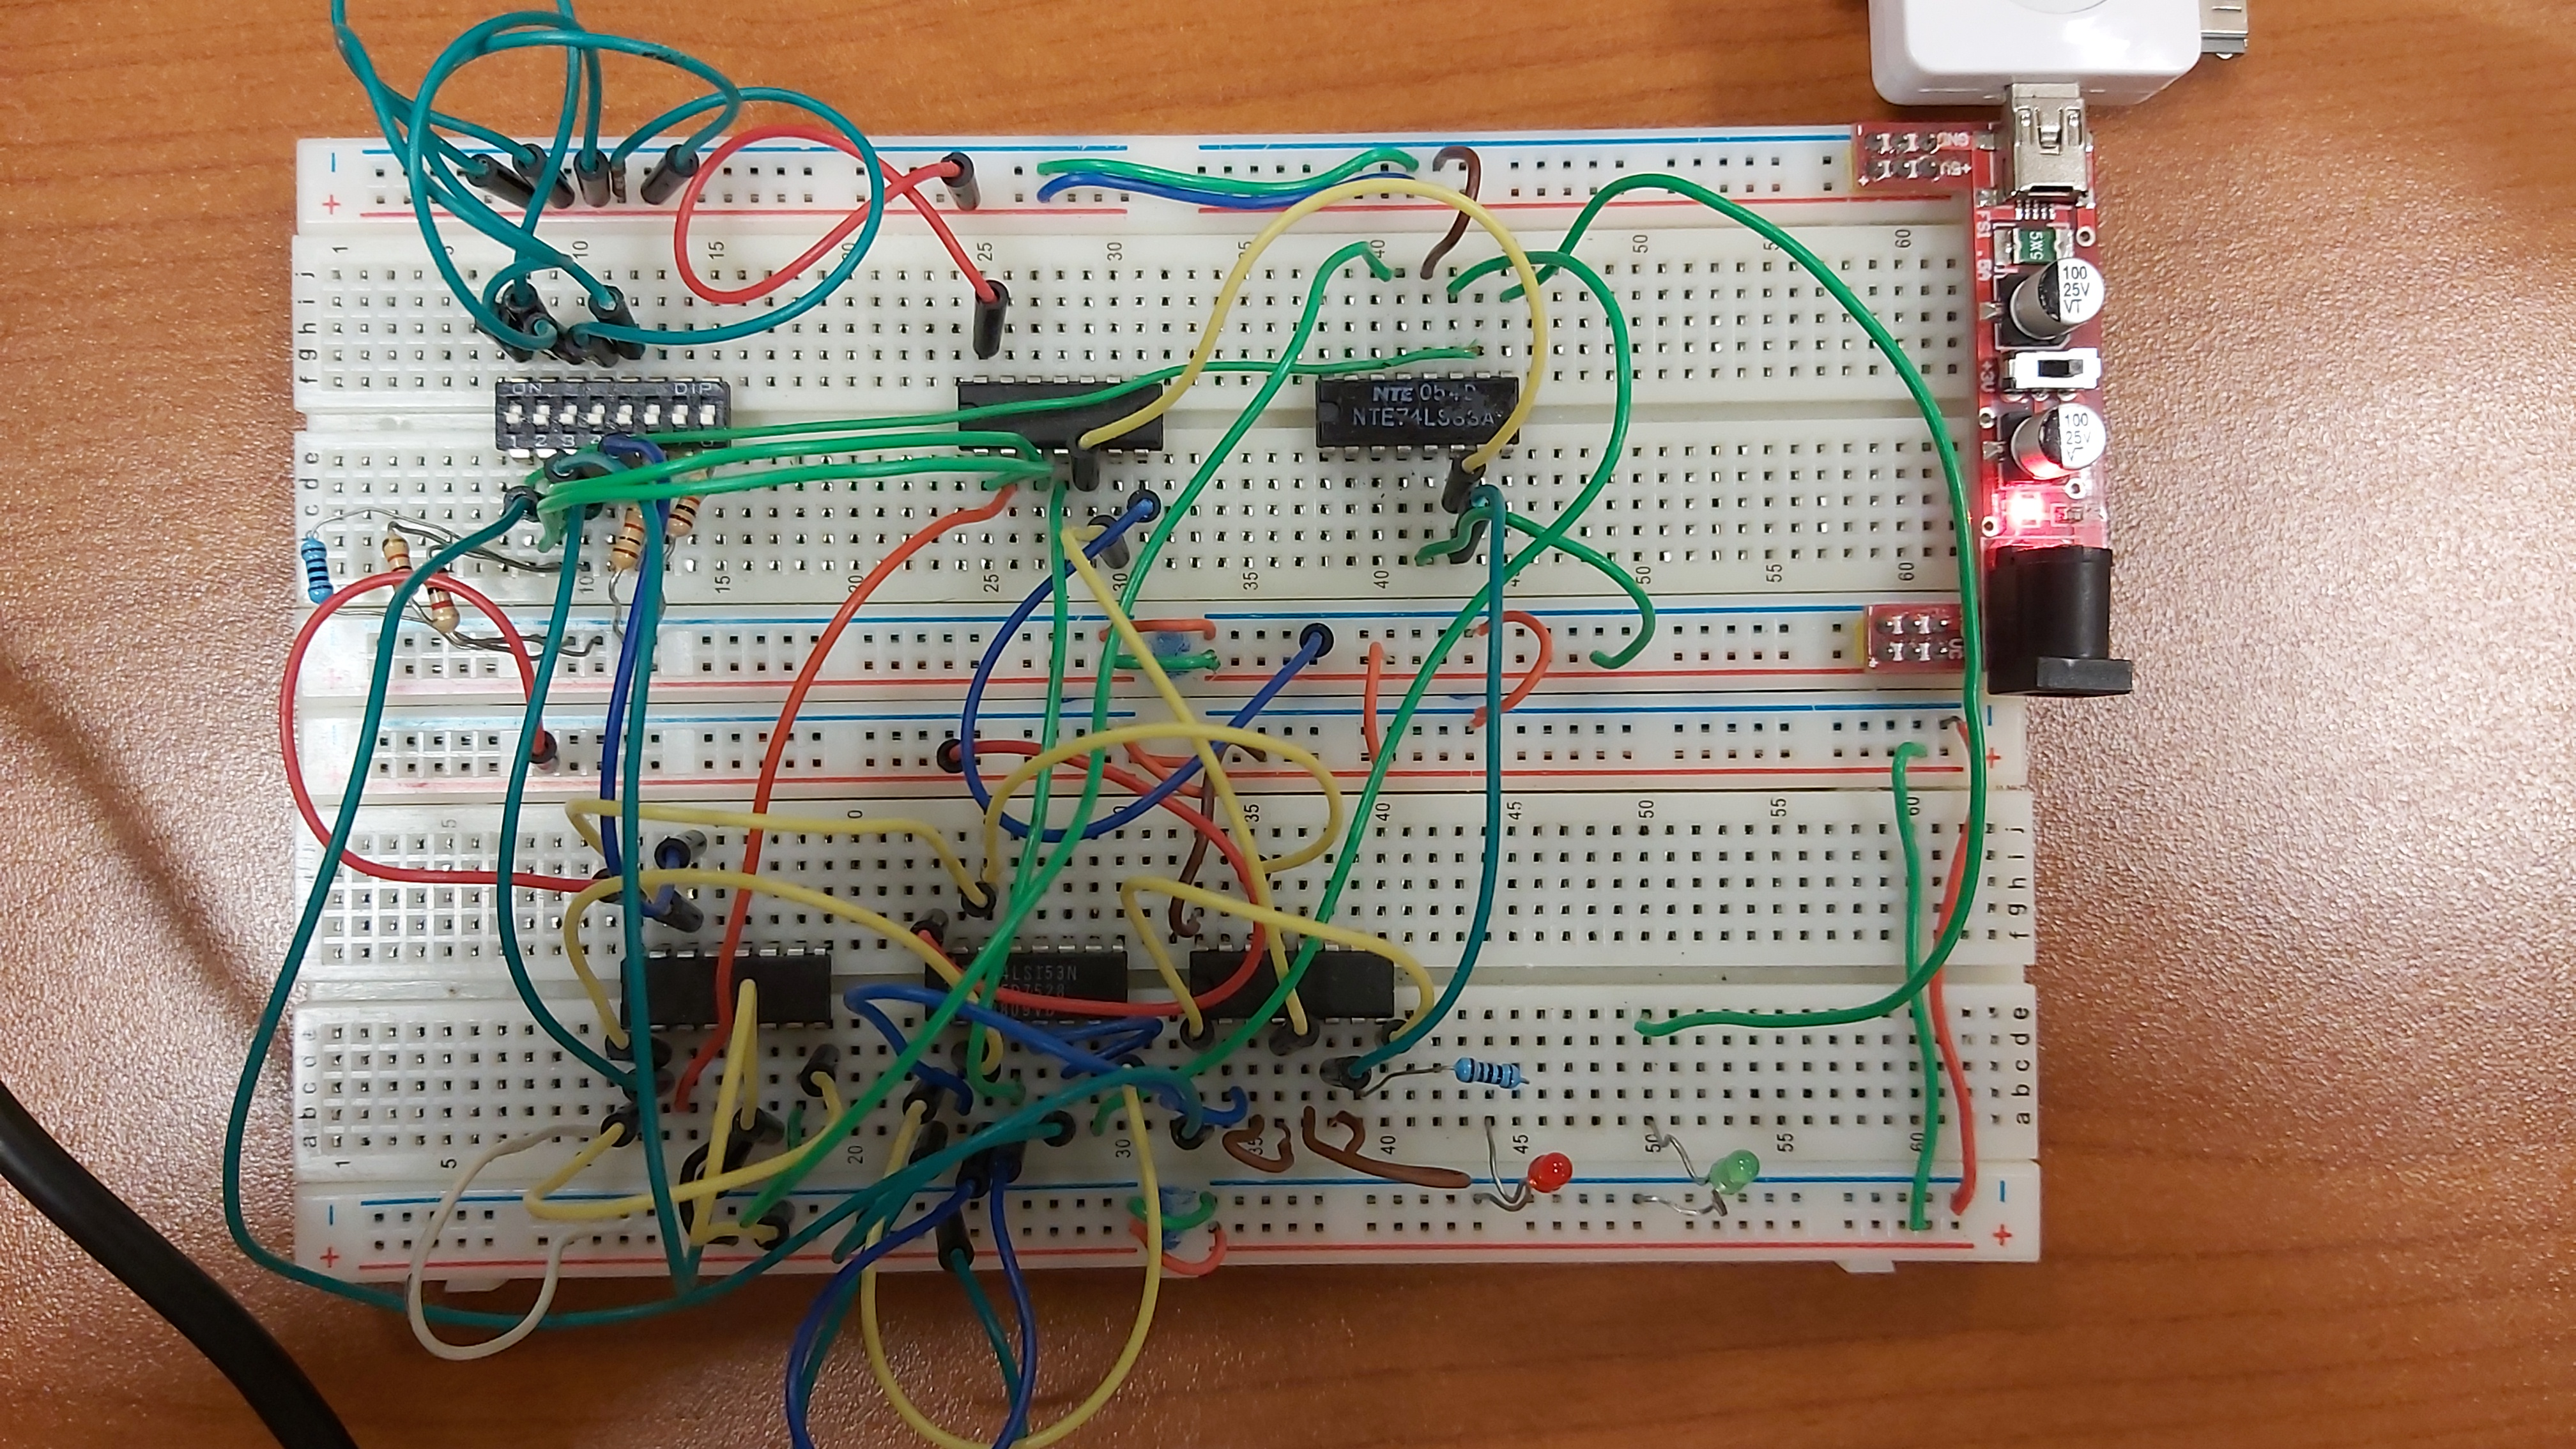
\includegraphics[width=\textwidth]{./figures/00000.jpg}
\begin{center}
	All inputs are off, and thus no LED is on.
\end{center}

\vspace{2em}

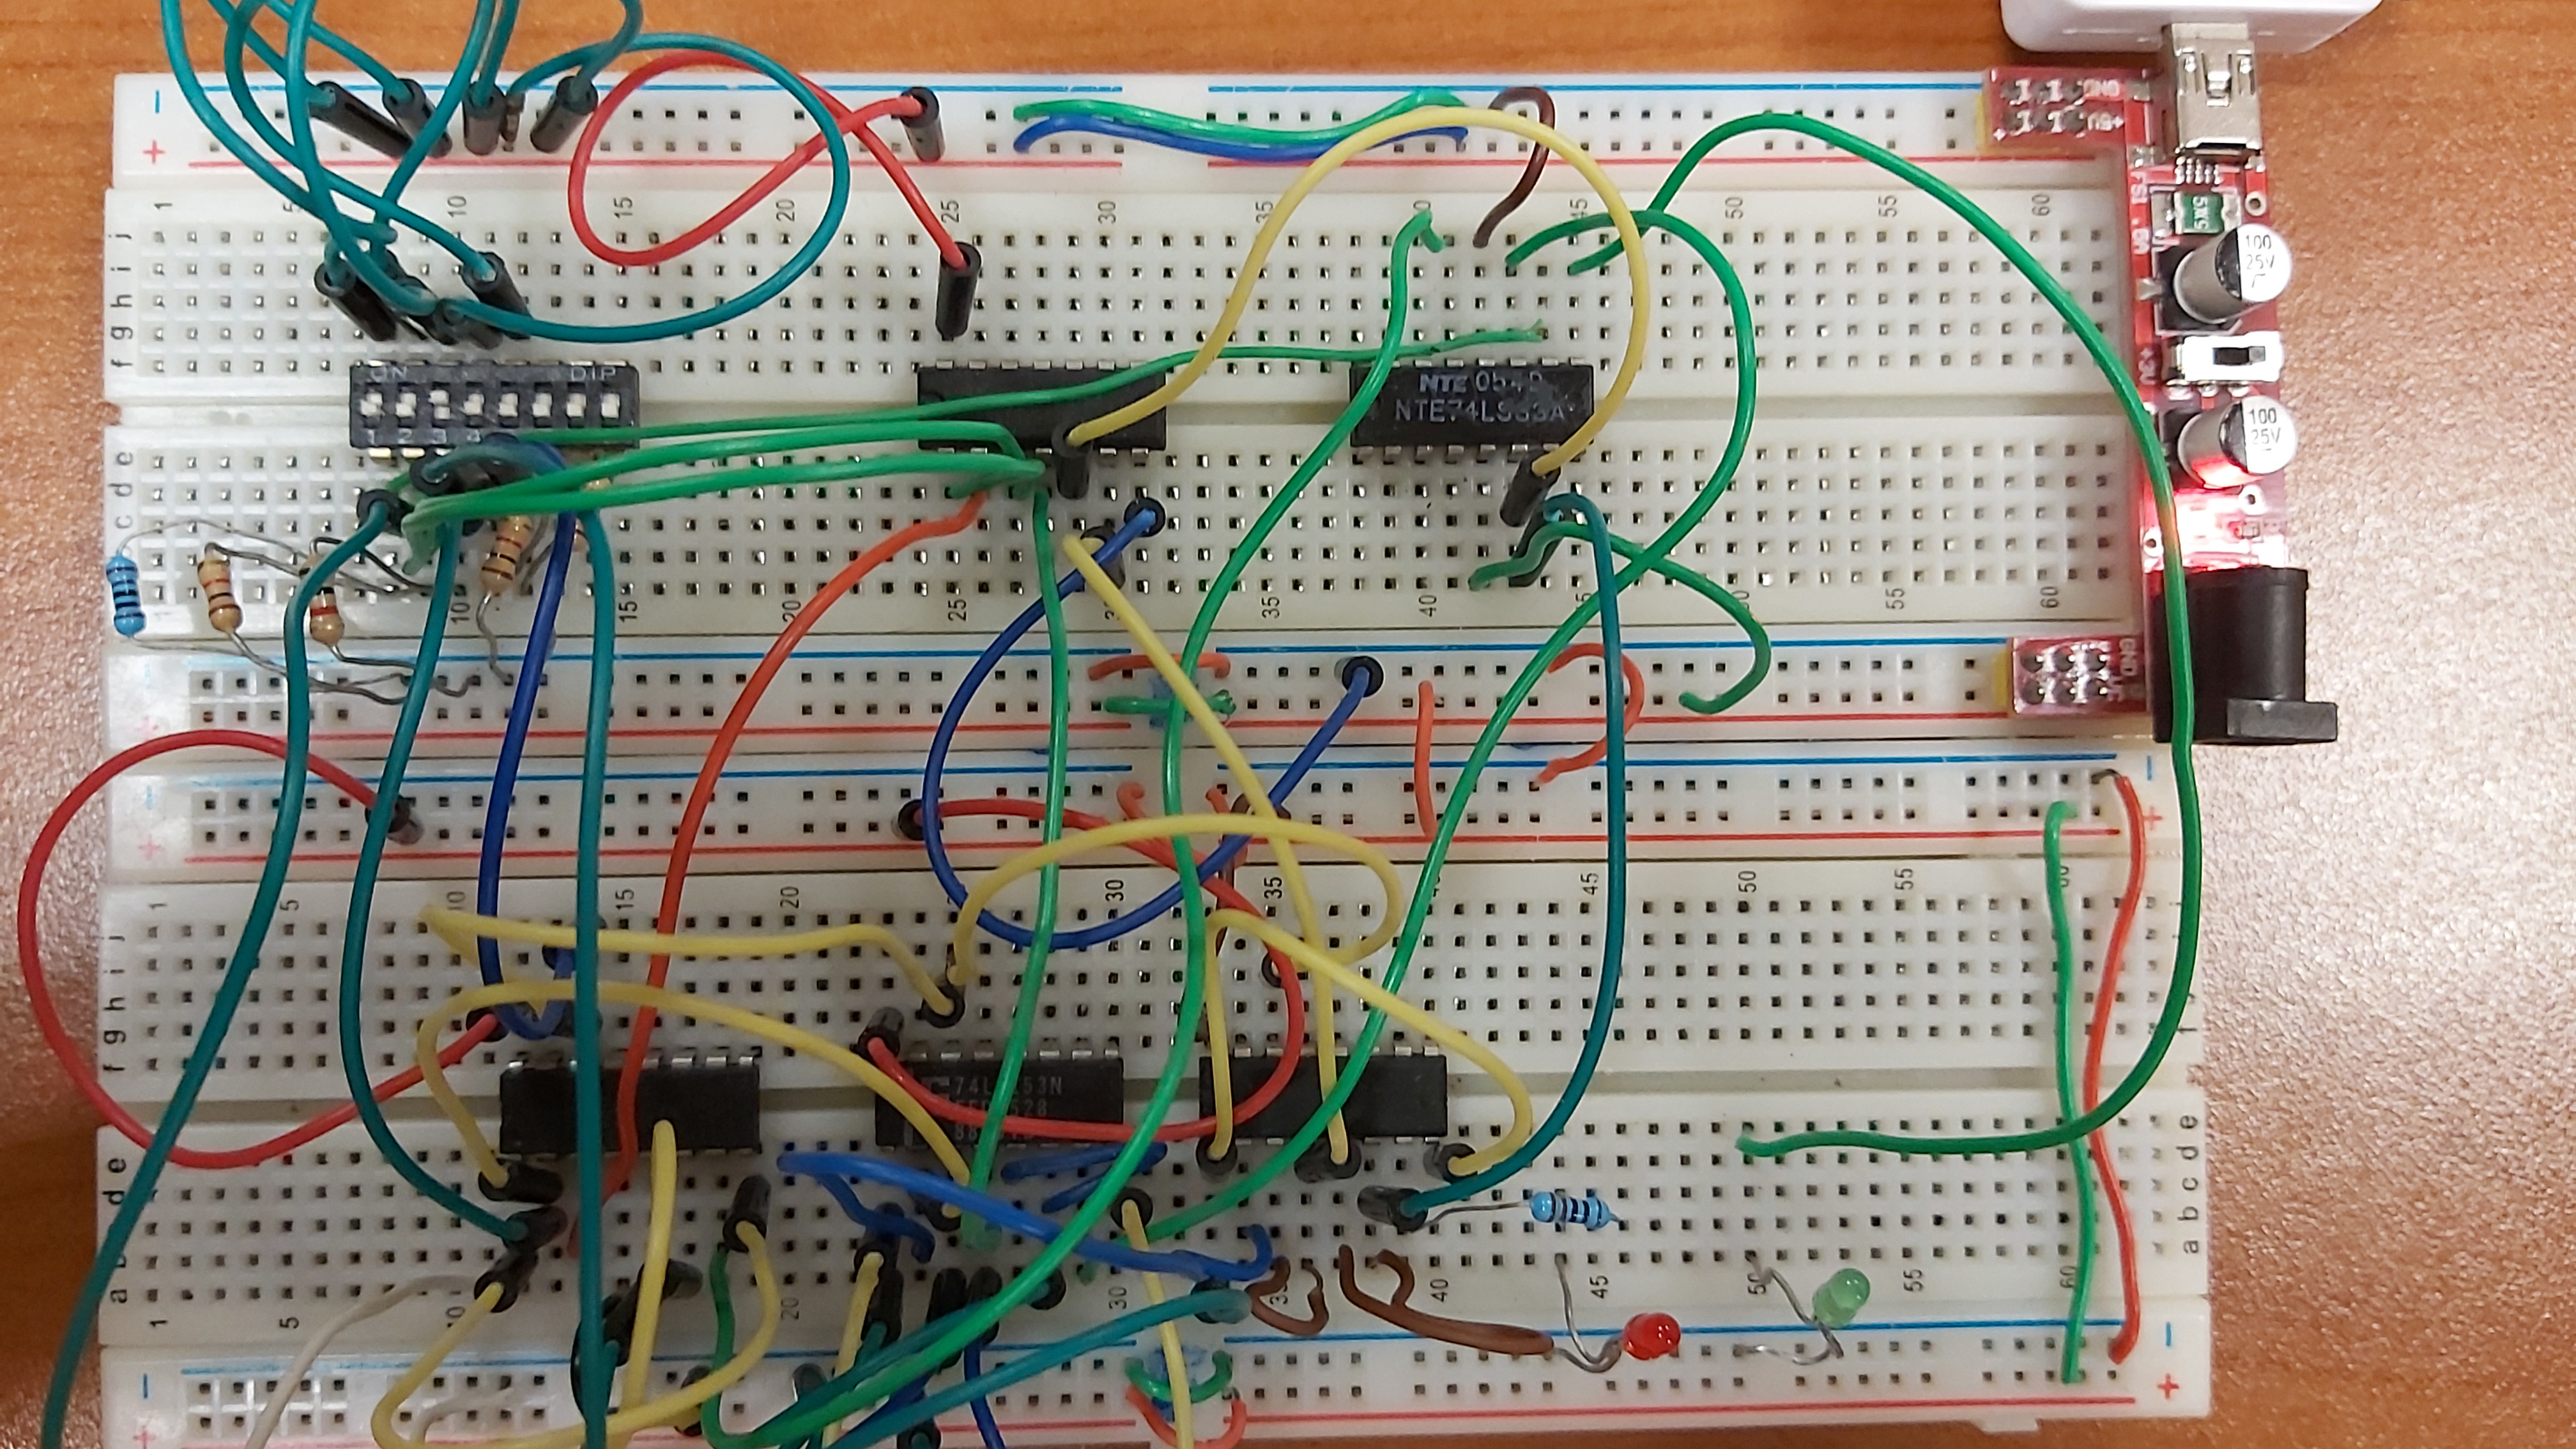
\includegraphics[width=\textwidth]{./figures/00100.jpg}
\begin{center}
	$ABC_i = 001$ and so $C_o Y= 00$.\\
\end{center}


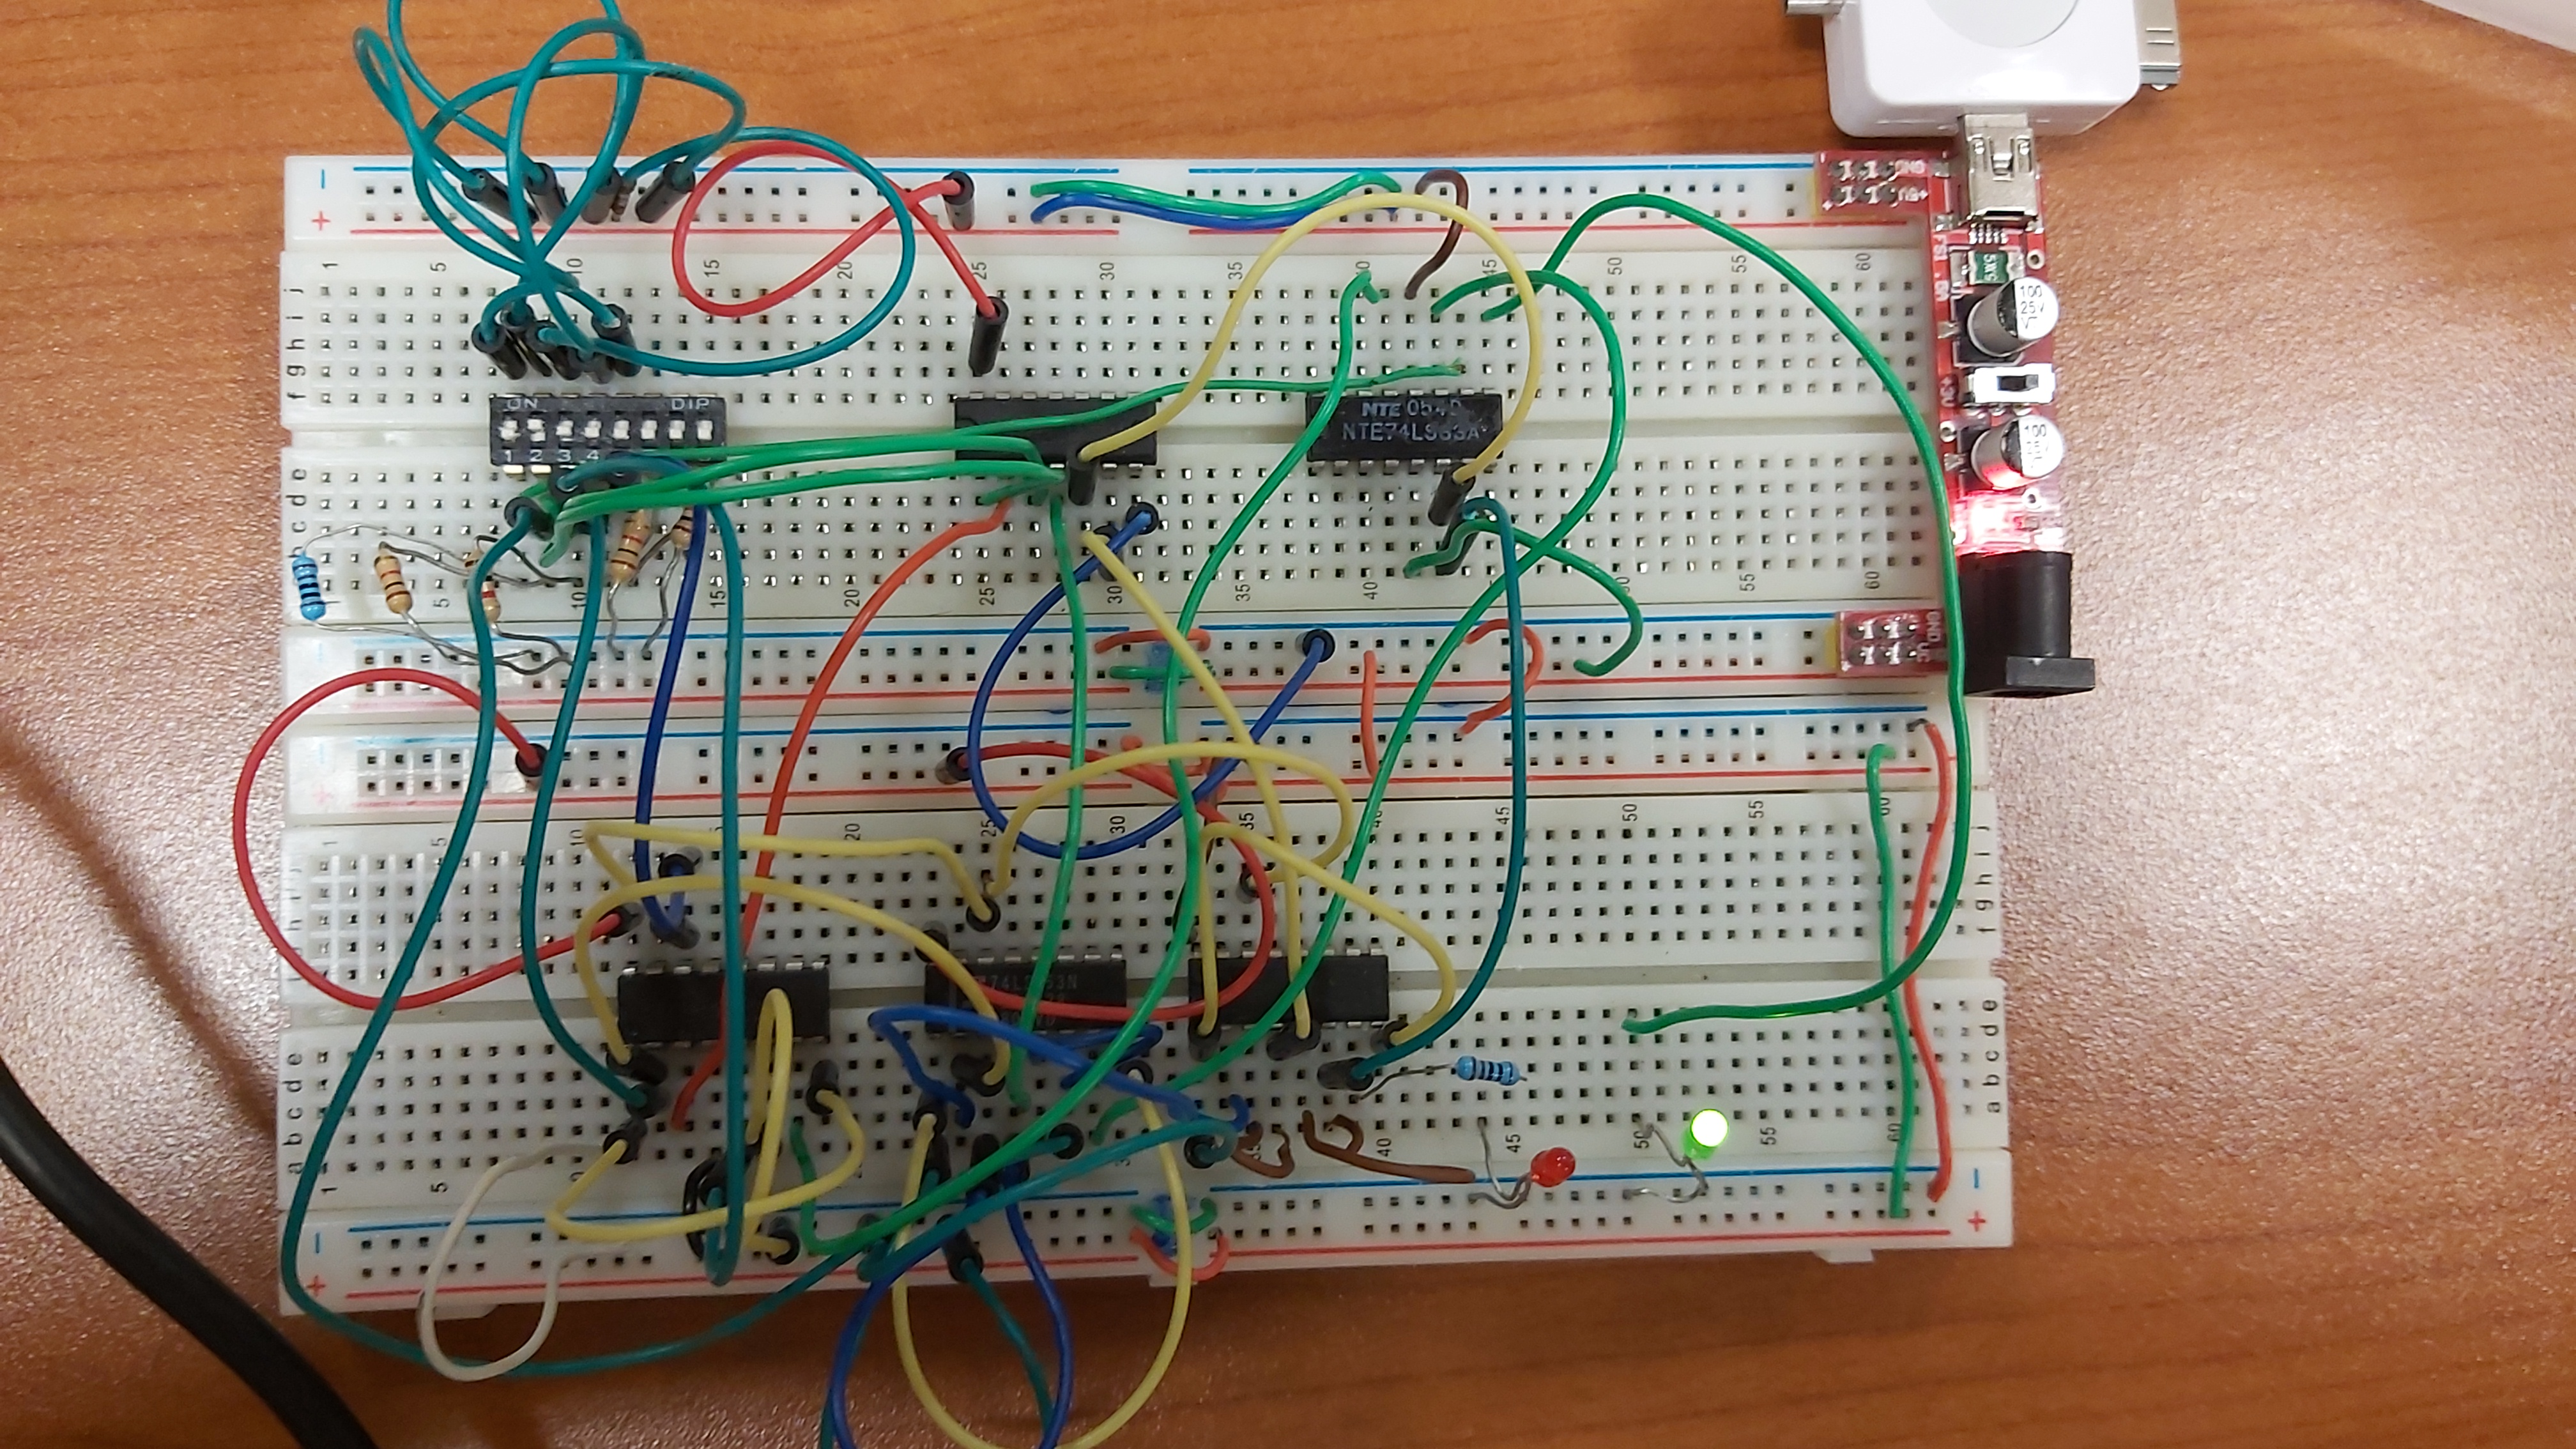
\includegraphics[width=\textwidth]{./figures/01000.jpg}
\begin{center}
	$ABC_i = 010$ and so $C_o Y= 01$.
\end{center}

\vspace{2em}

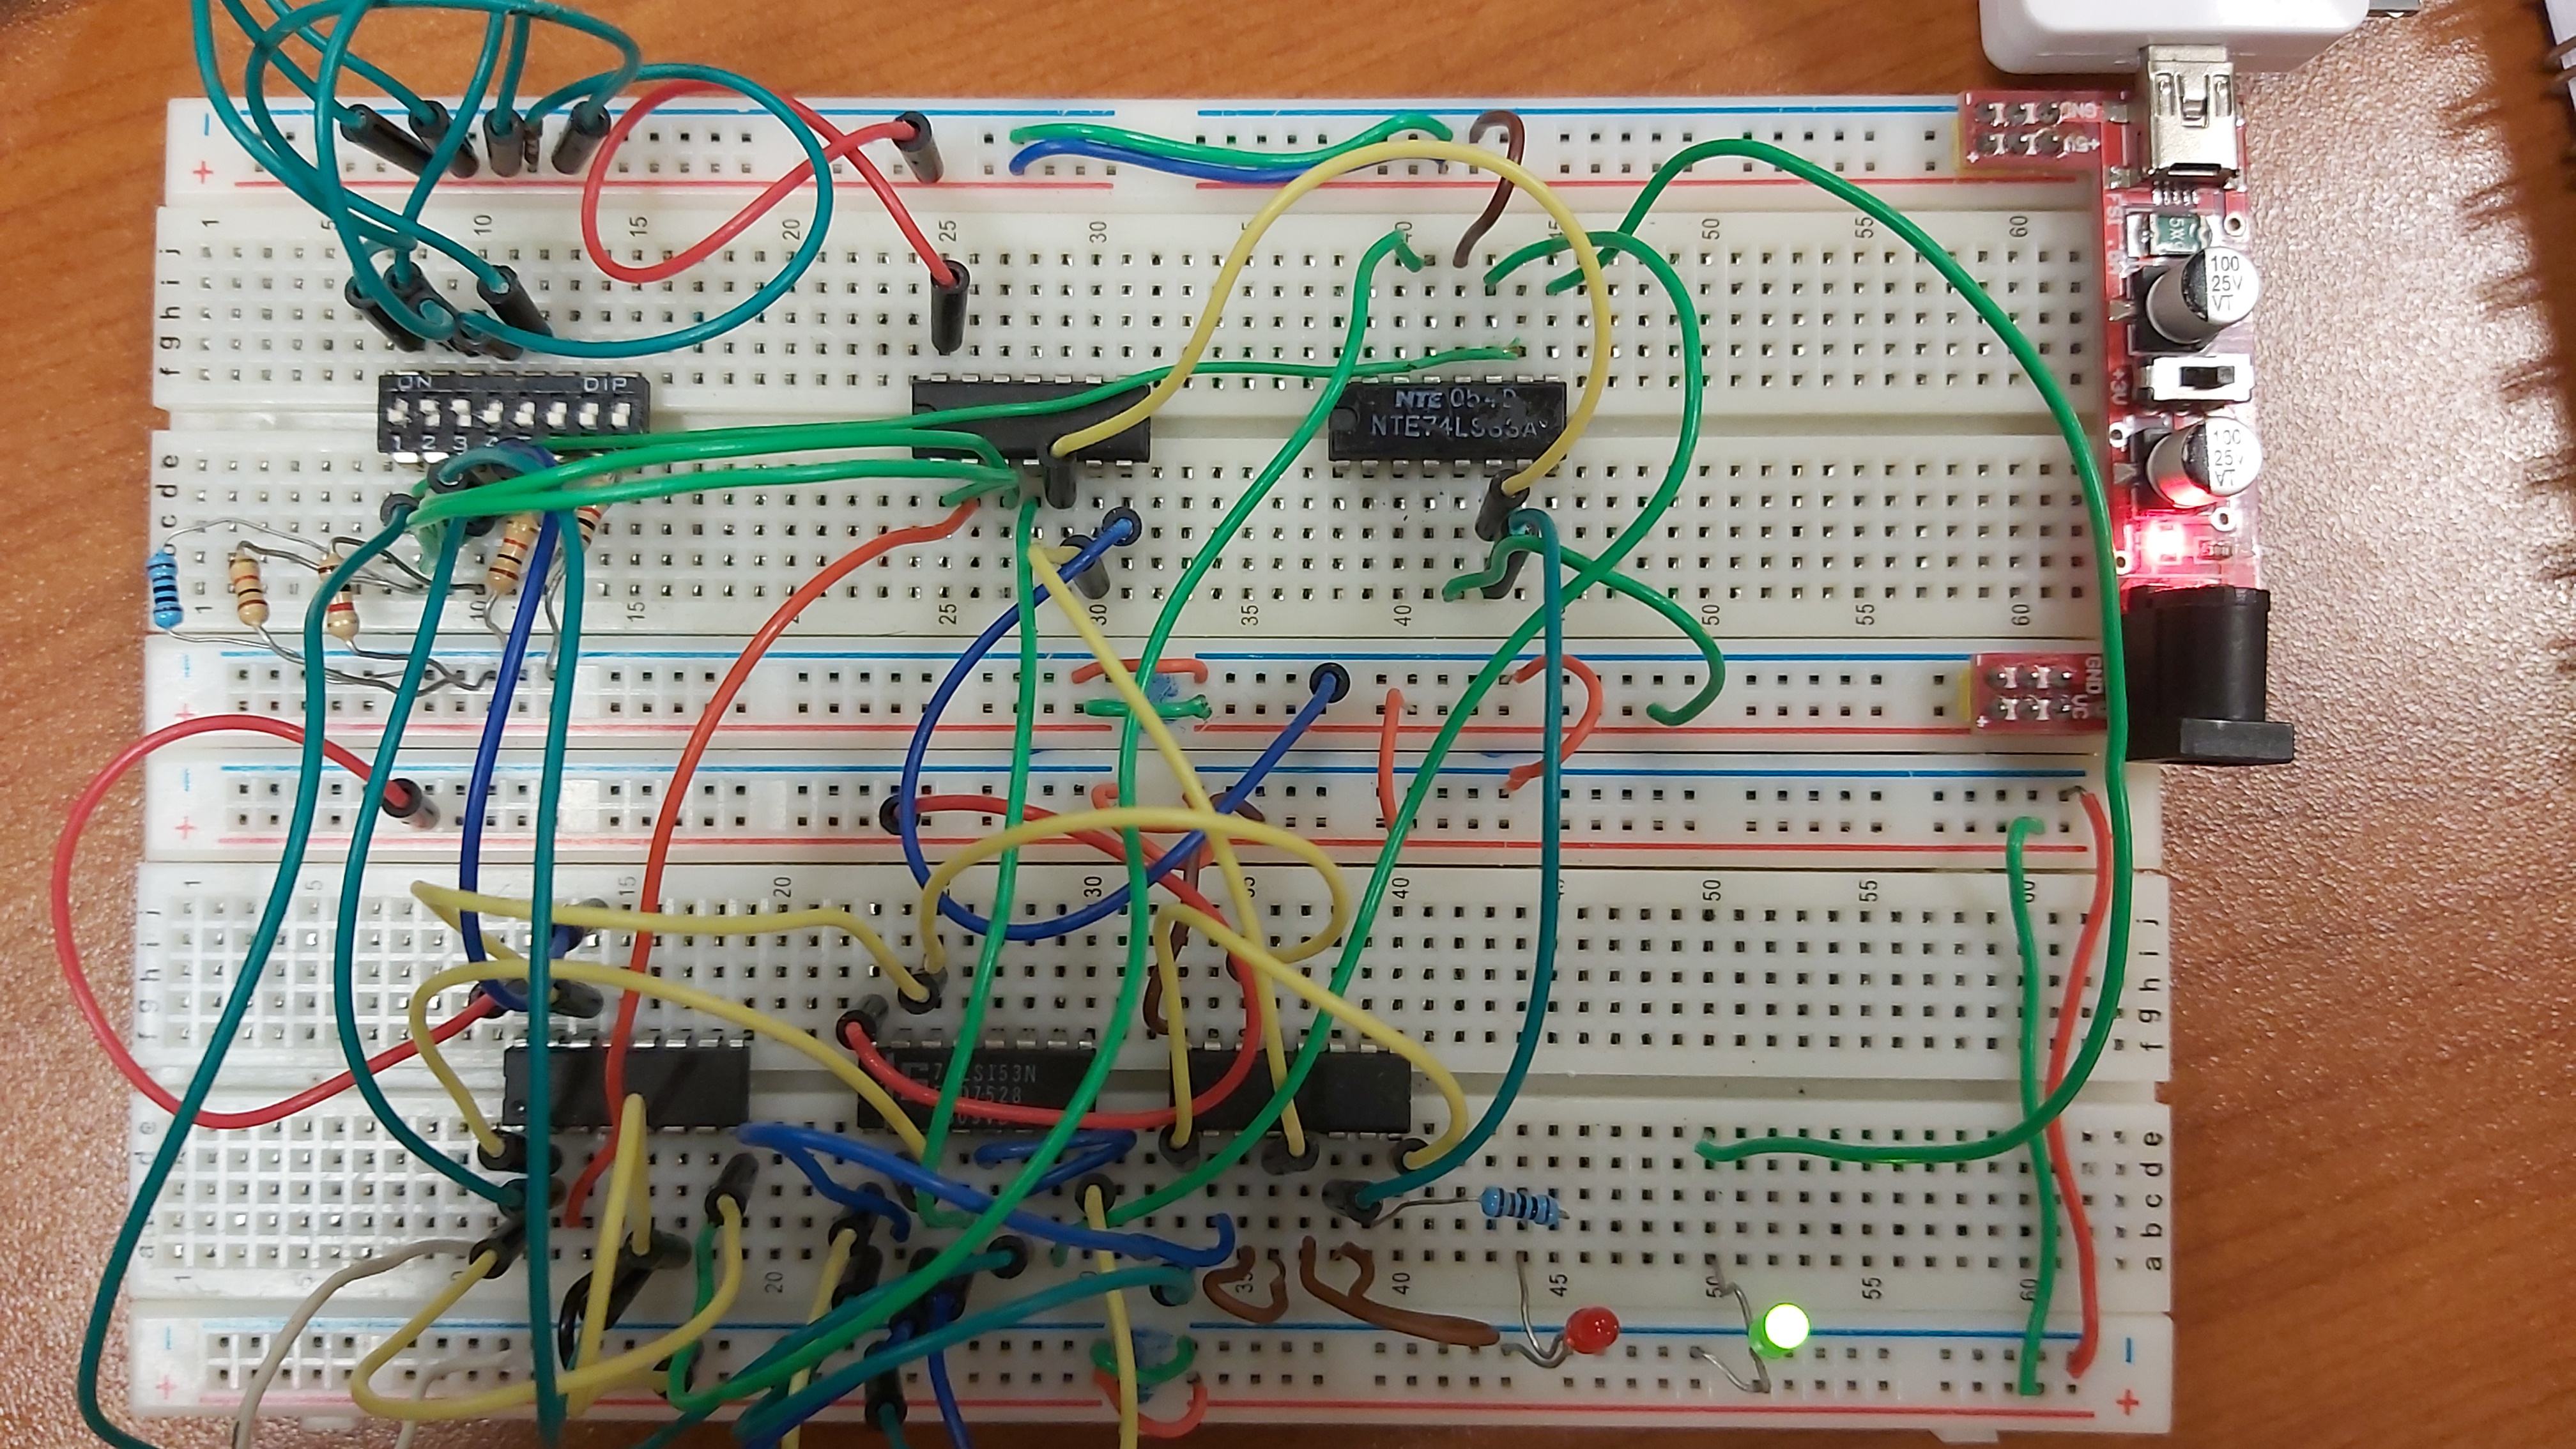
\includegraphics[width=\textwidth]{./figures/01100.jpg}
\begin{center}
	$ABC_i = 011$ and so $C_o Y= 01$.
\end{center}


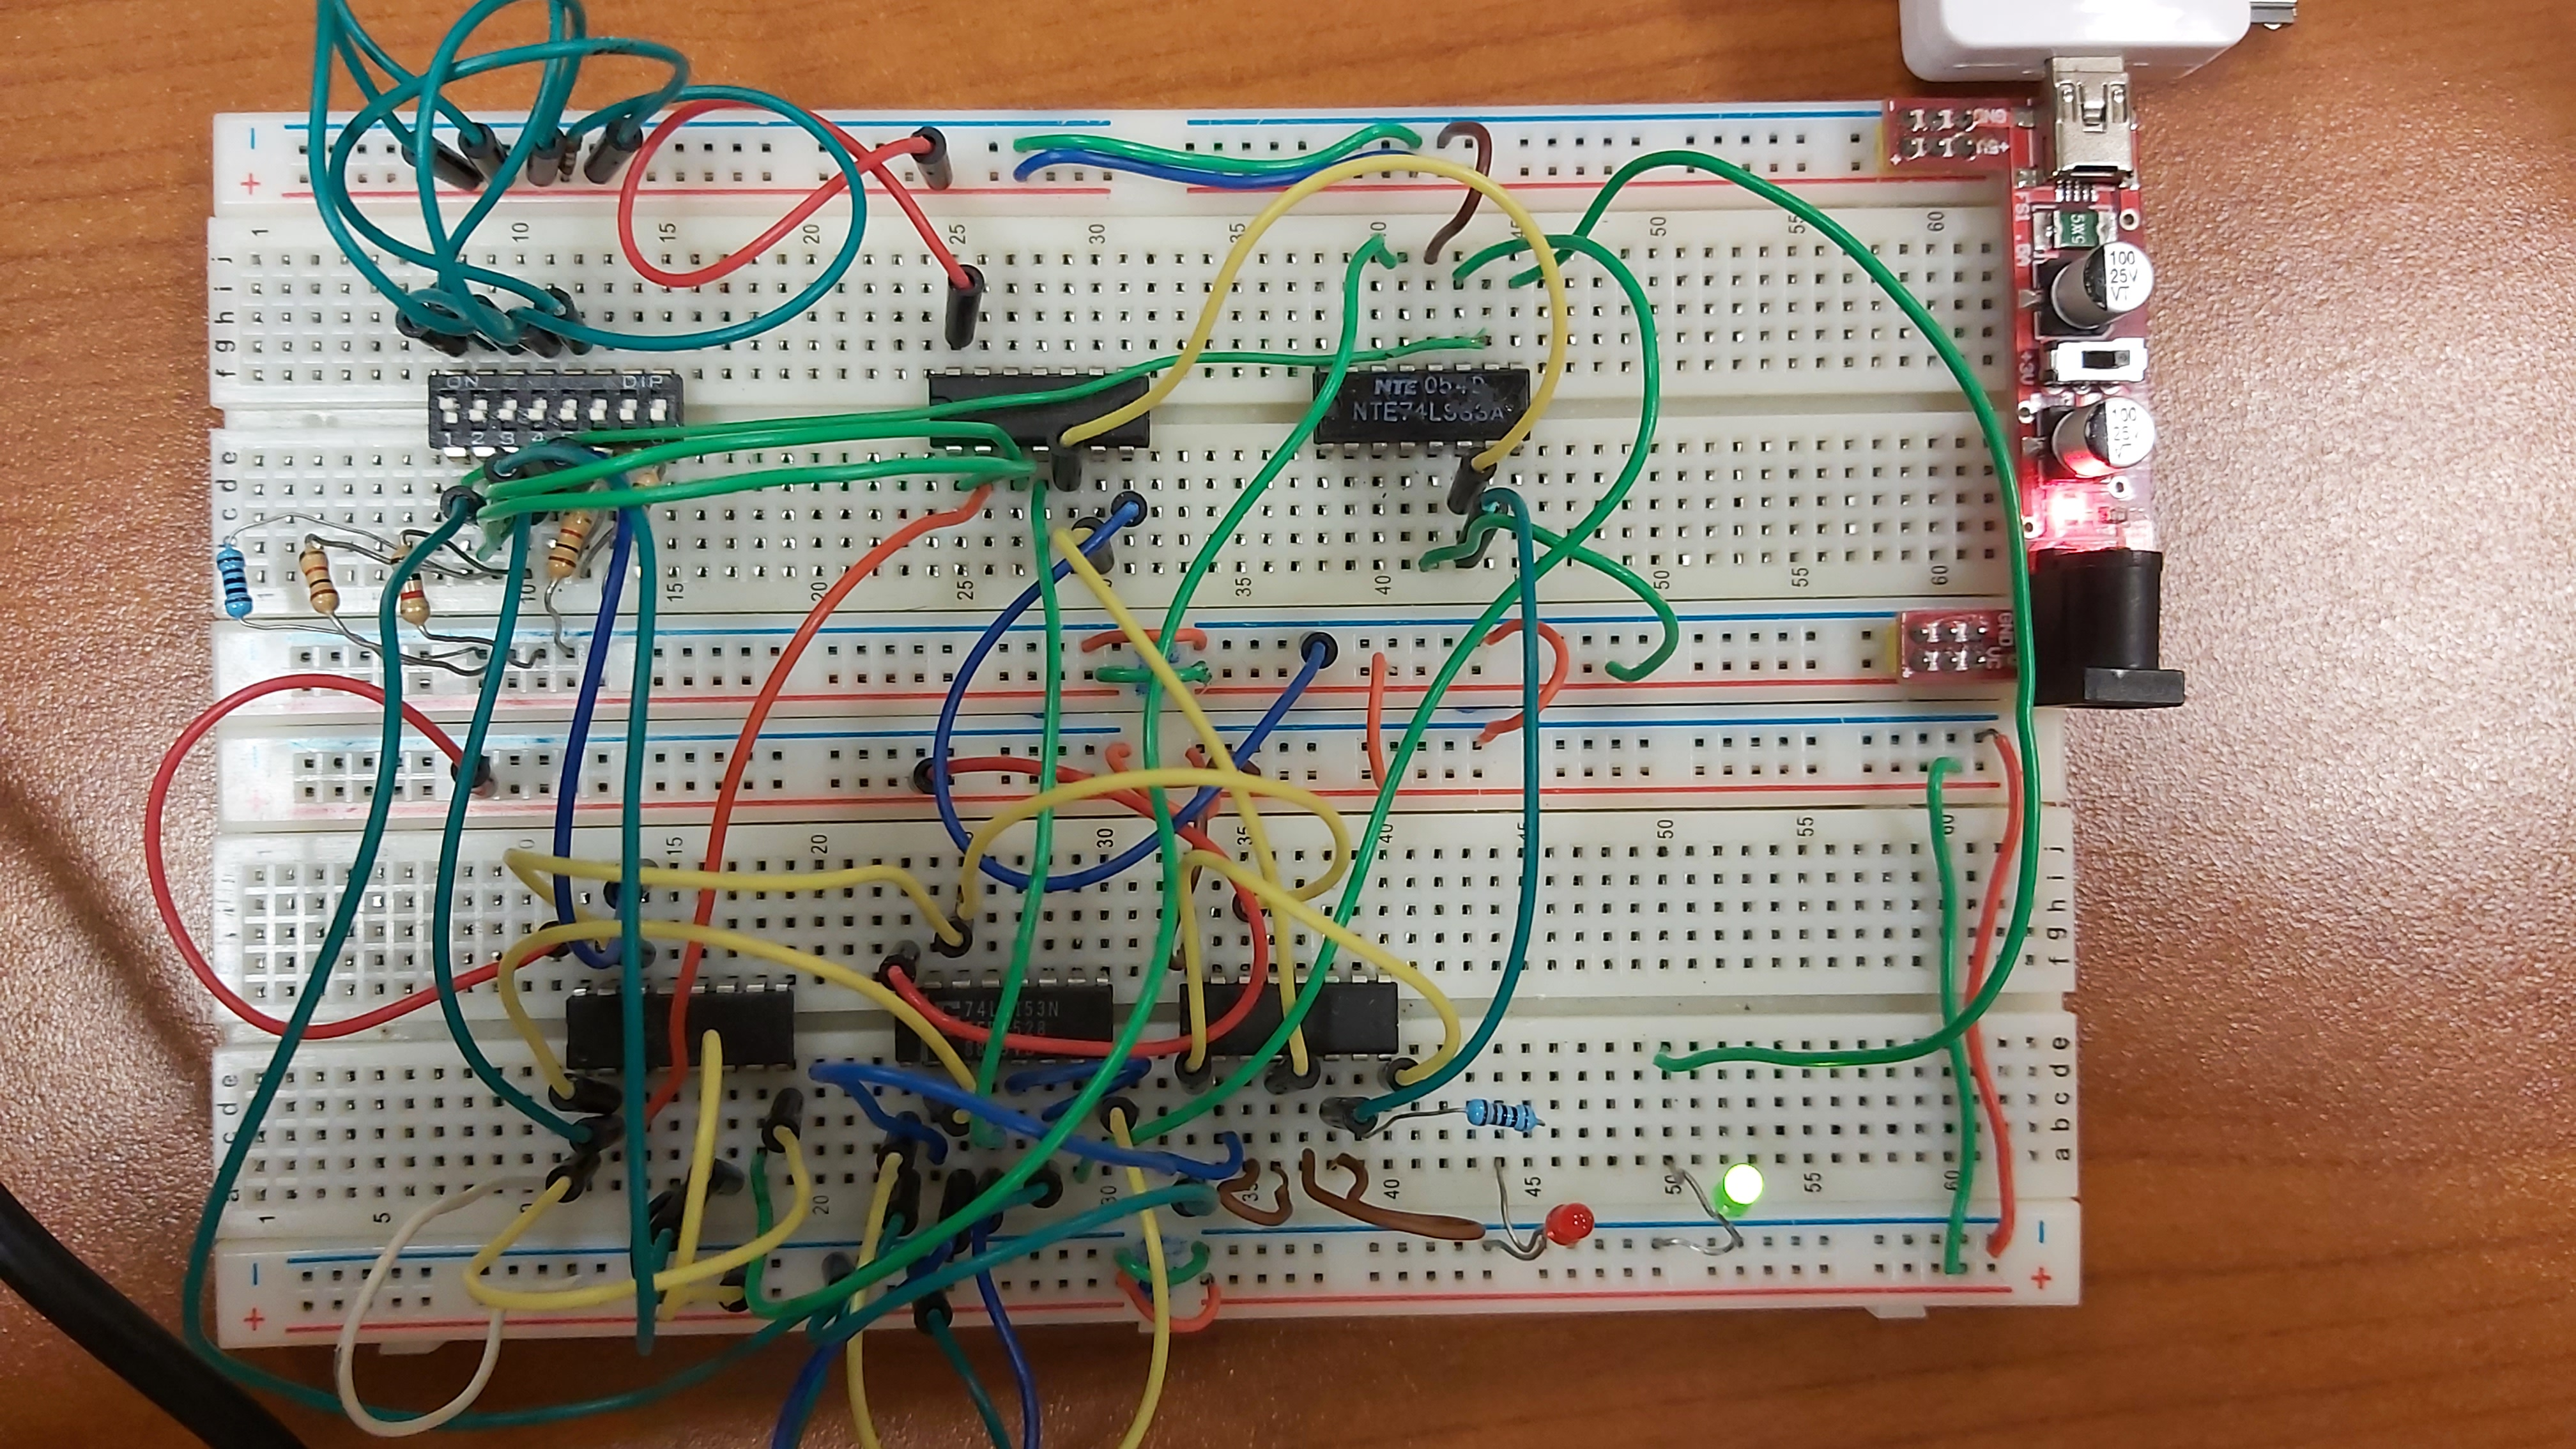
\includegraphics[width=\textwidth]{./figures/10000.jpg}
\begin{center}
	$ABC_i = 100$ and so $C_o Y= 01$.
\end{center}

\vspace{2em}

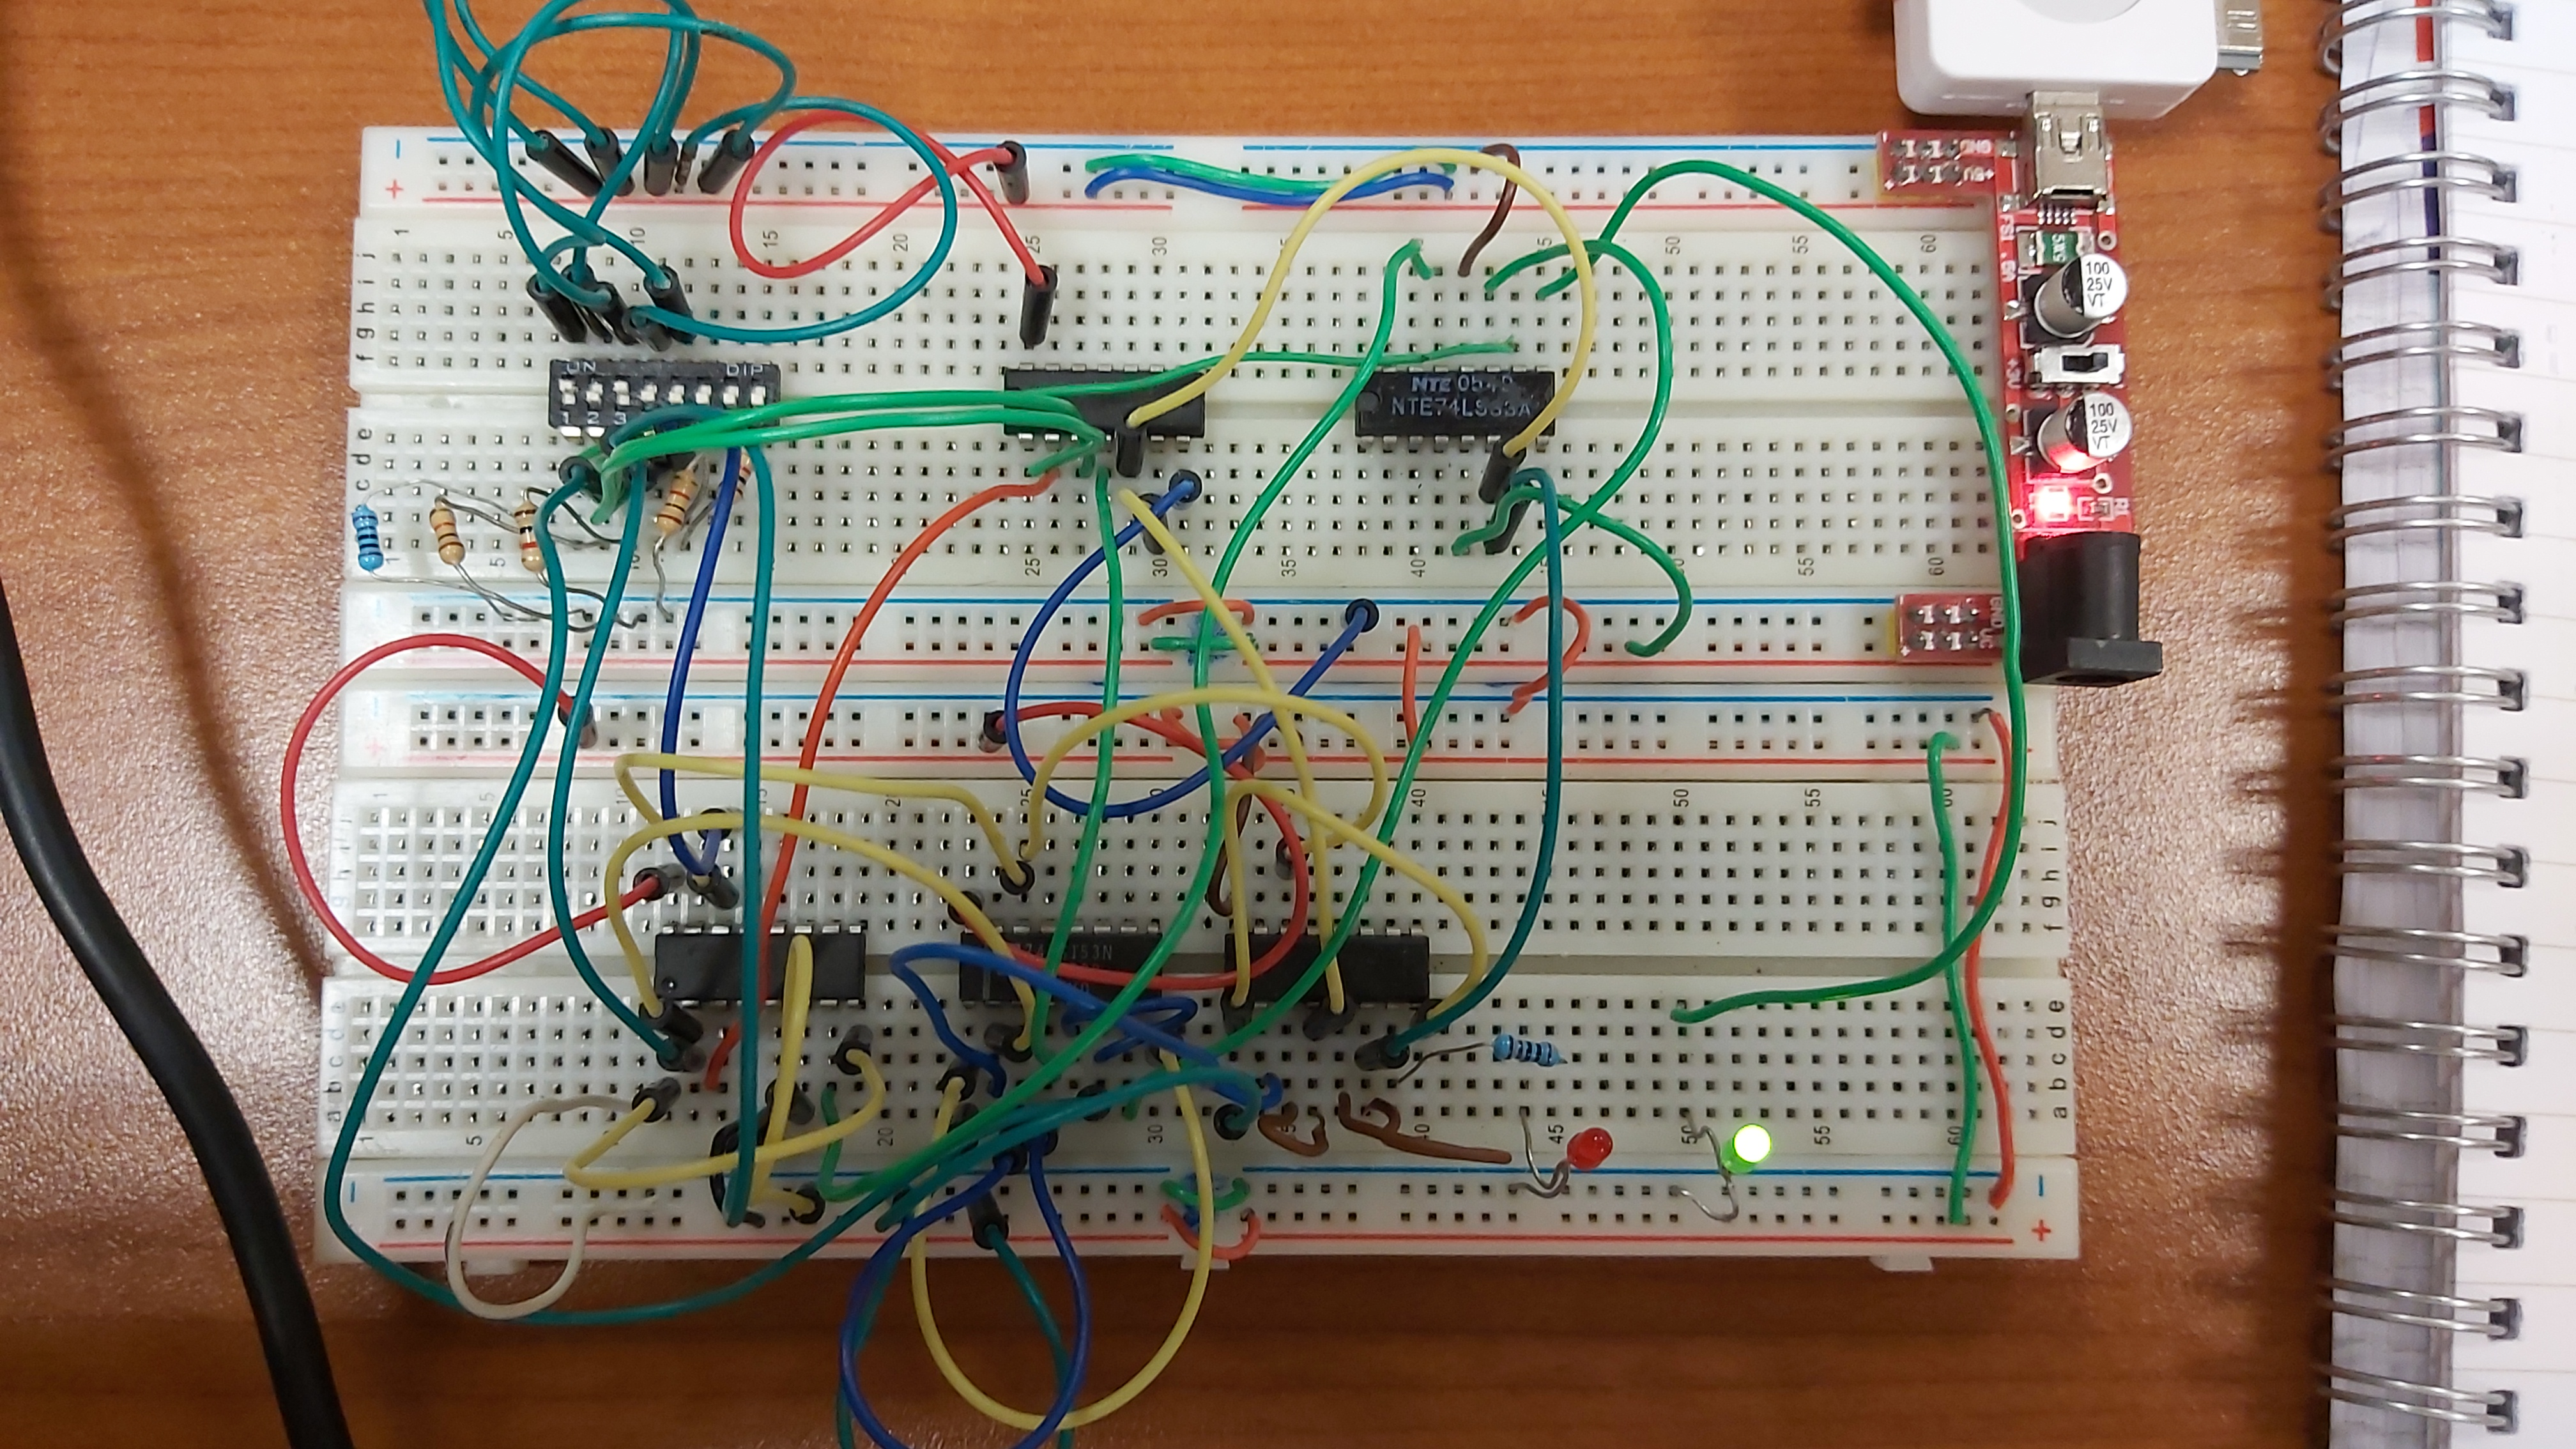
\includegraphics[width=\textwidth]{./figures/10100.jpg}
\begin{center}
	$ABC_i = 101$ and so $C_o Y= 01$.
\end{center}


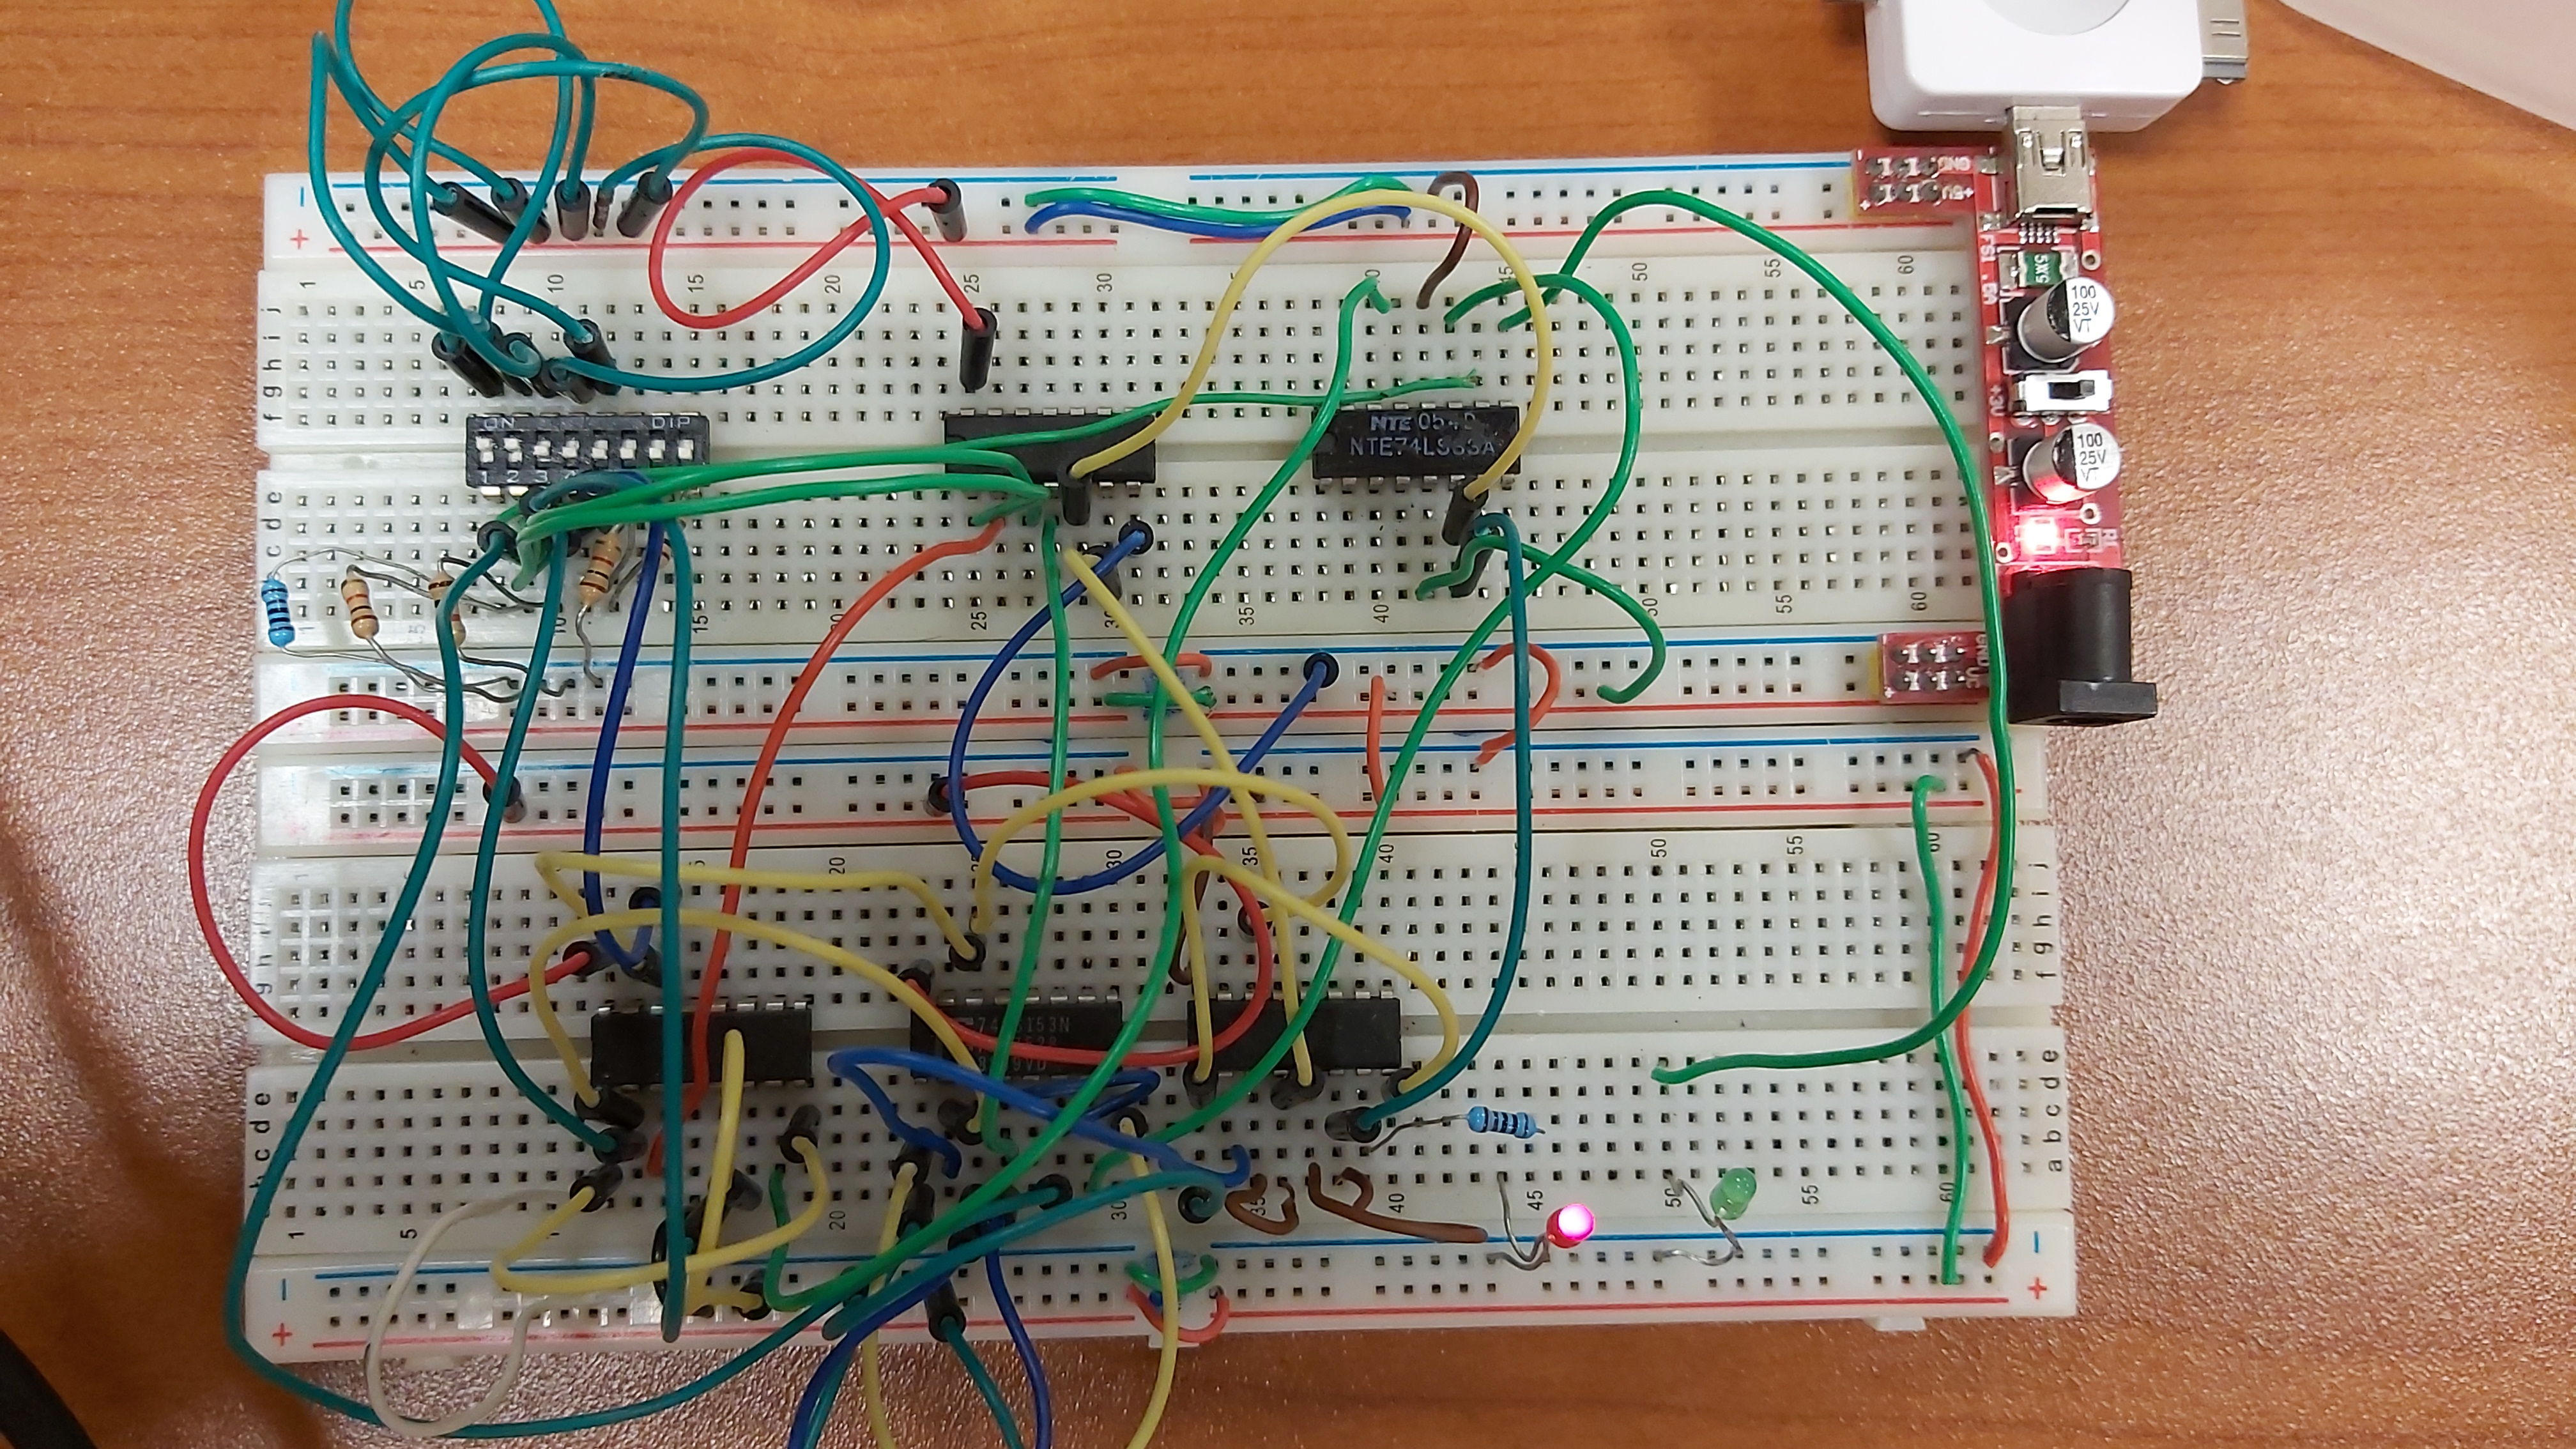
\includegraphics[width=\textwidth]{./figures/11000.jpg}
\begin{center}
	$ABC_i = 110$ and so $C_o Y= 10$.
\end{center}

\vspace{2em}

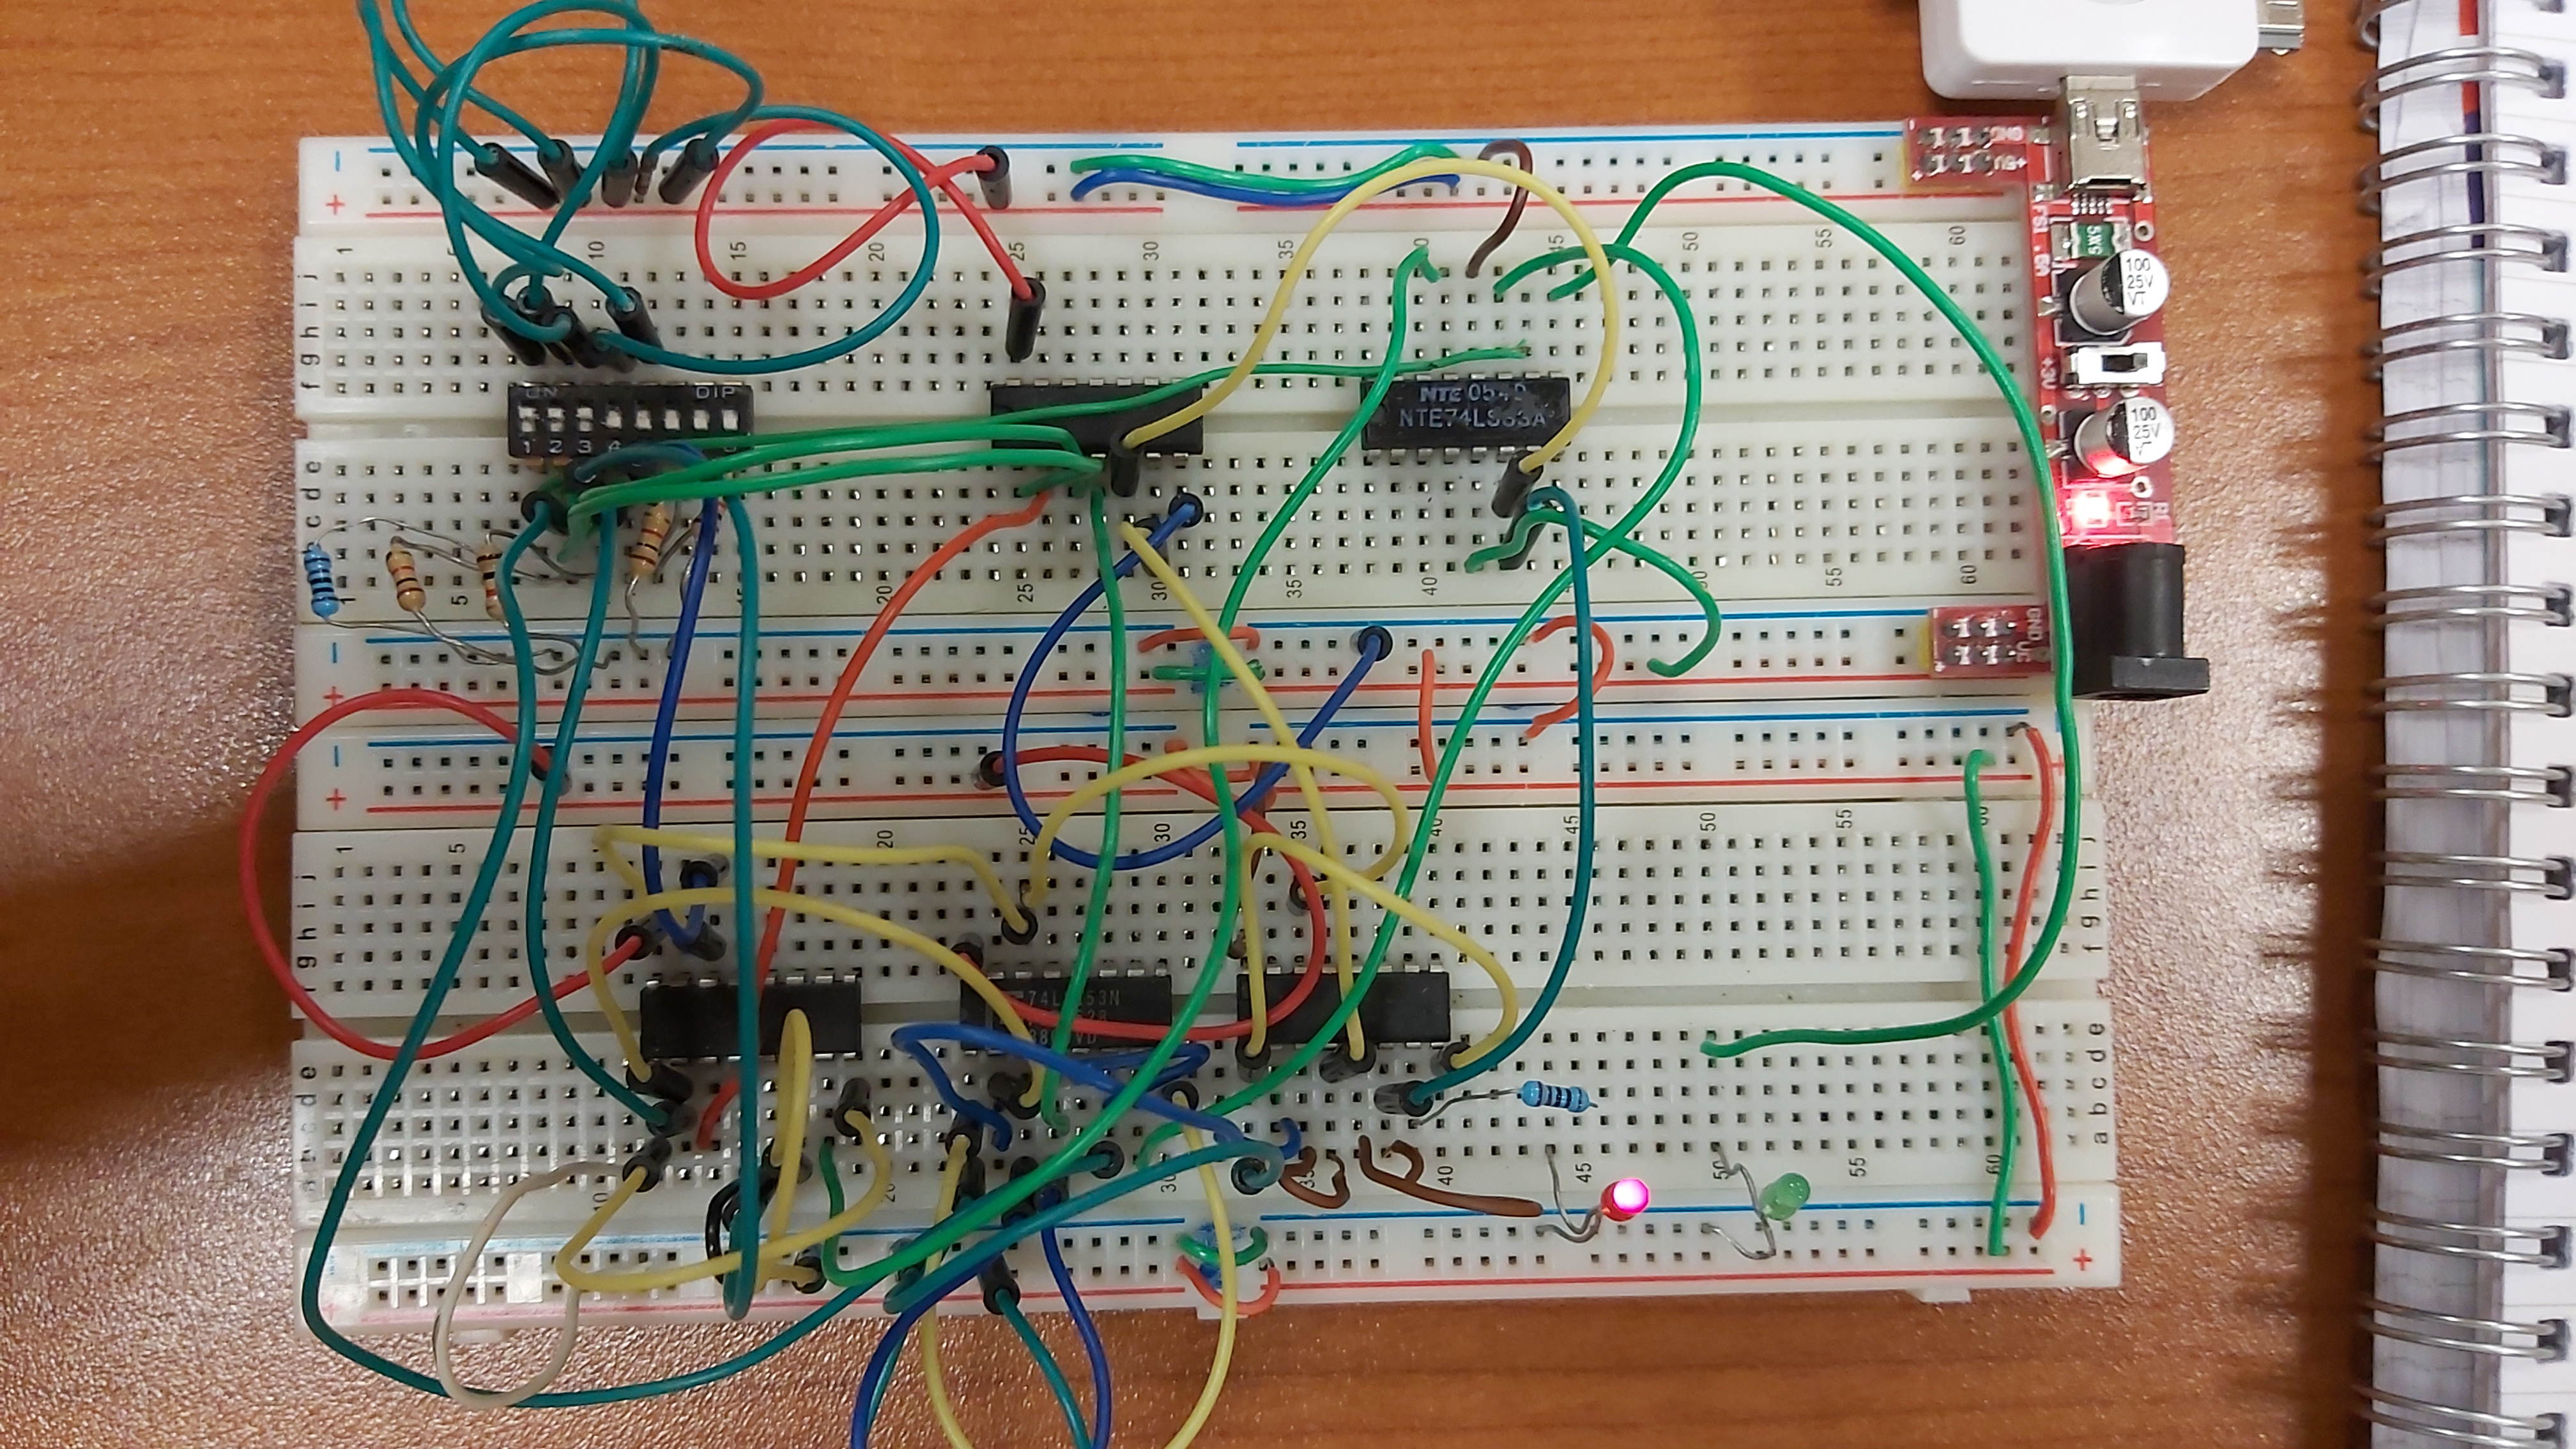
\includegraphics[width=\textwidth]{./figures/11100.jpg}
\begin{center}
	$ABC_i = 111$ and so $C_o Y= 10$.
\end{center}


\subsection{Opcode \texttt{01 - ADDC}}

With this opcode selected, the ALU performs the addition of bits $A$ and $B$ but consequently
adding the carry bit represented by $C_i$.

\[A+B+C_i = C_o Y\]

\vspace{9em}

\subsubsection{Truth table}

\begin{center}
	\Large
	\begin{tabular}{c|c|c||c|c||c|c|c}
		$A$ & $B$ & $C_i$ & $Op_1$ & $Op_2$ & $C_{o}$ & $Y$ \\
		\hline
		0 & 0 & 0 & 0 & 1 & 0 & 0 \\
		0 & 0 & 1 & 0 & 1 & 0 & 0 \\
		0 & 1 & 0 & 0 & 1 & 0 & 1 \\
		0 & 1 & 1 & 0 & 1 & 0 & 1 \\
		1 & 0 & 0 & 0 & 1 & 0 & 1 \\
		1 & 0 & 1 & 0 & 1 & 0 & 1 \\
		1 & 1 & 0 & 0 & 1 & 1 & 0 \\
		1 & 1 & 1 & 0 & 1 & 1 & 0 \\
	\end{tabular}
\end{center}


\newpage

\subsubsection{Pictures}


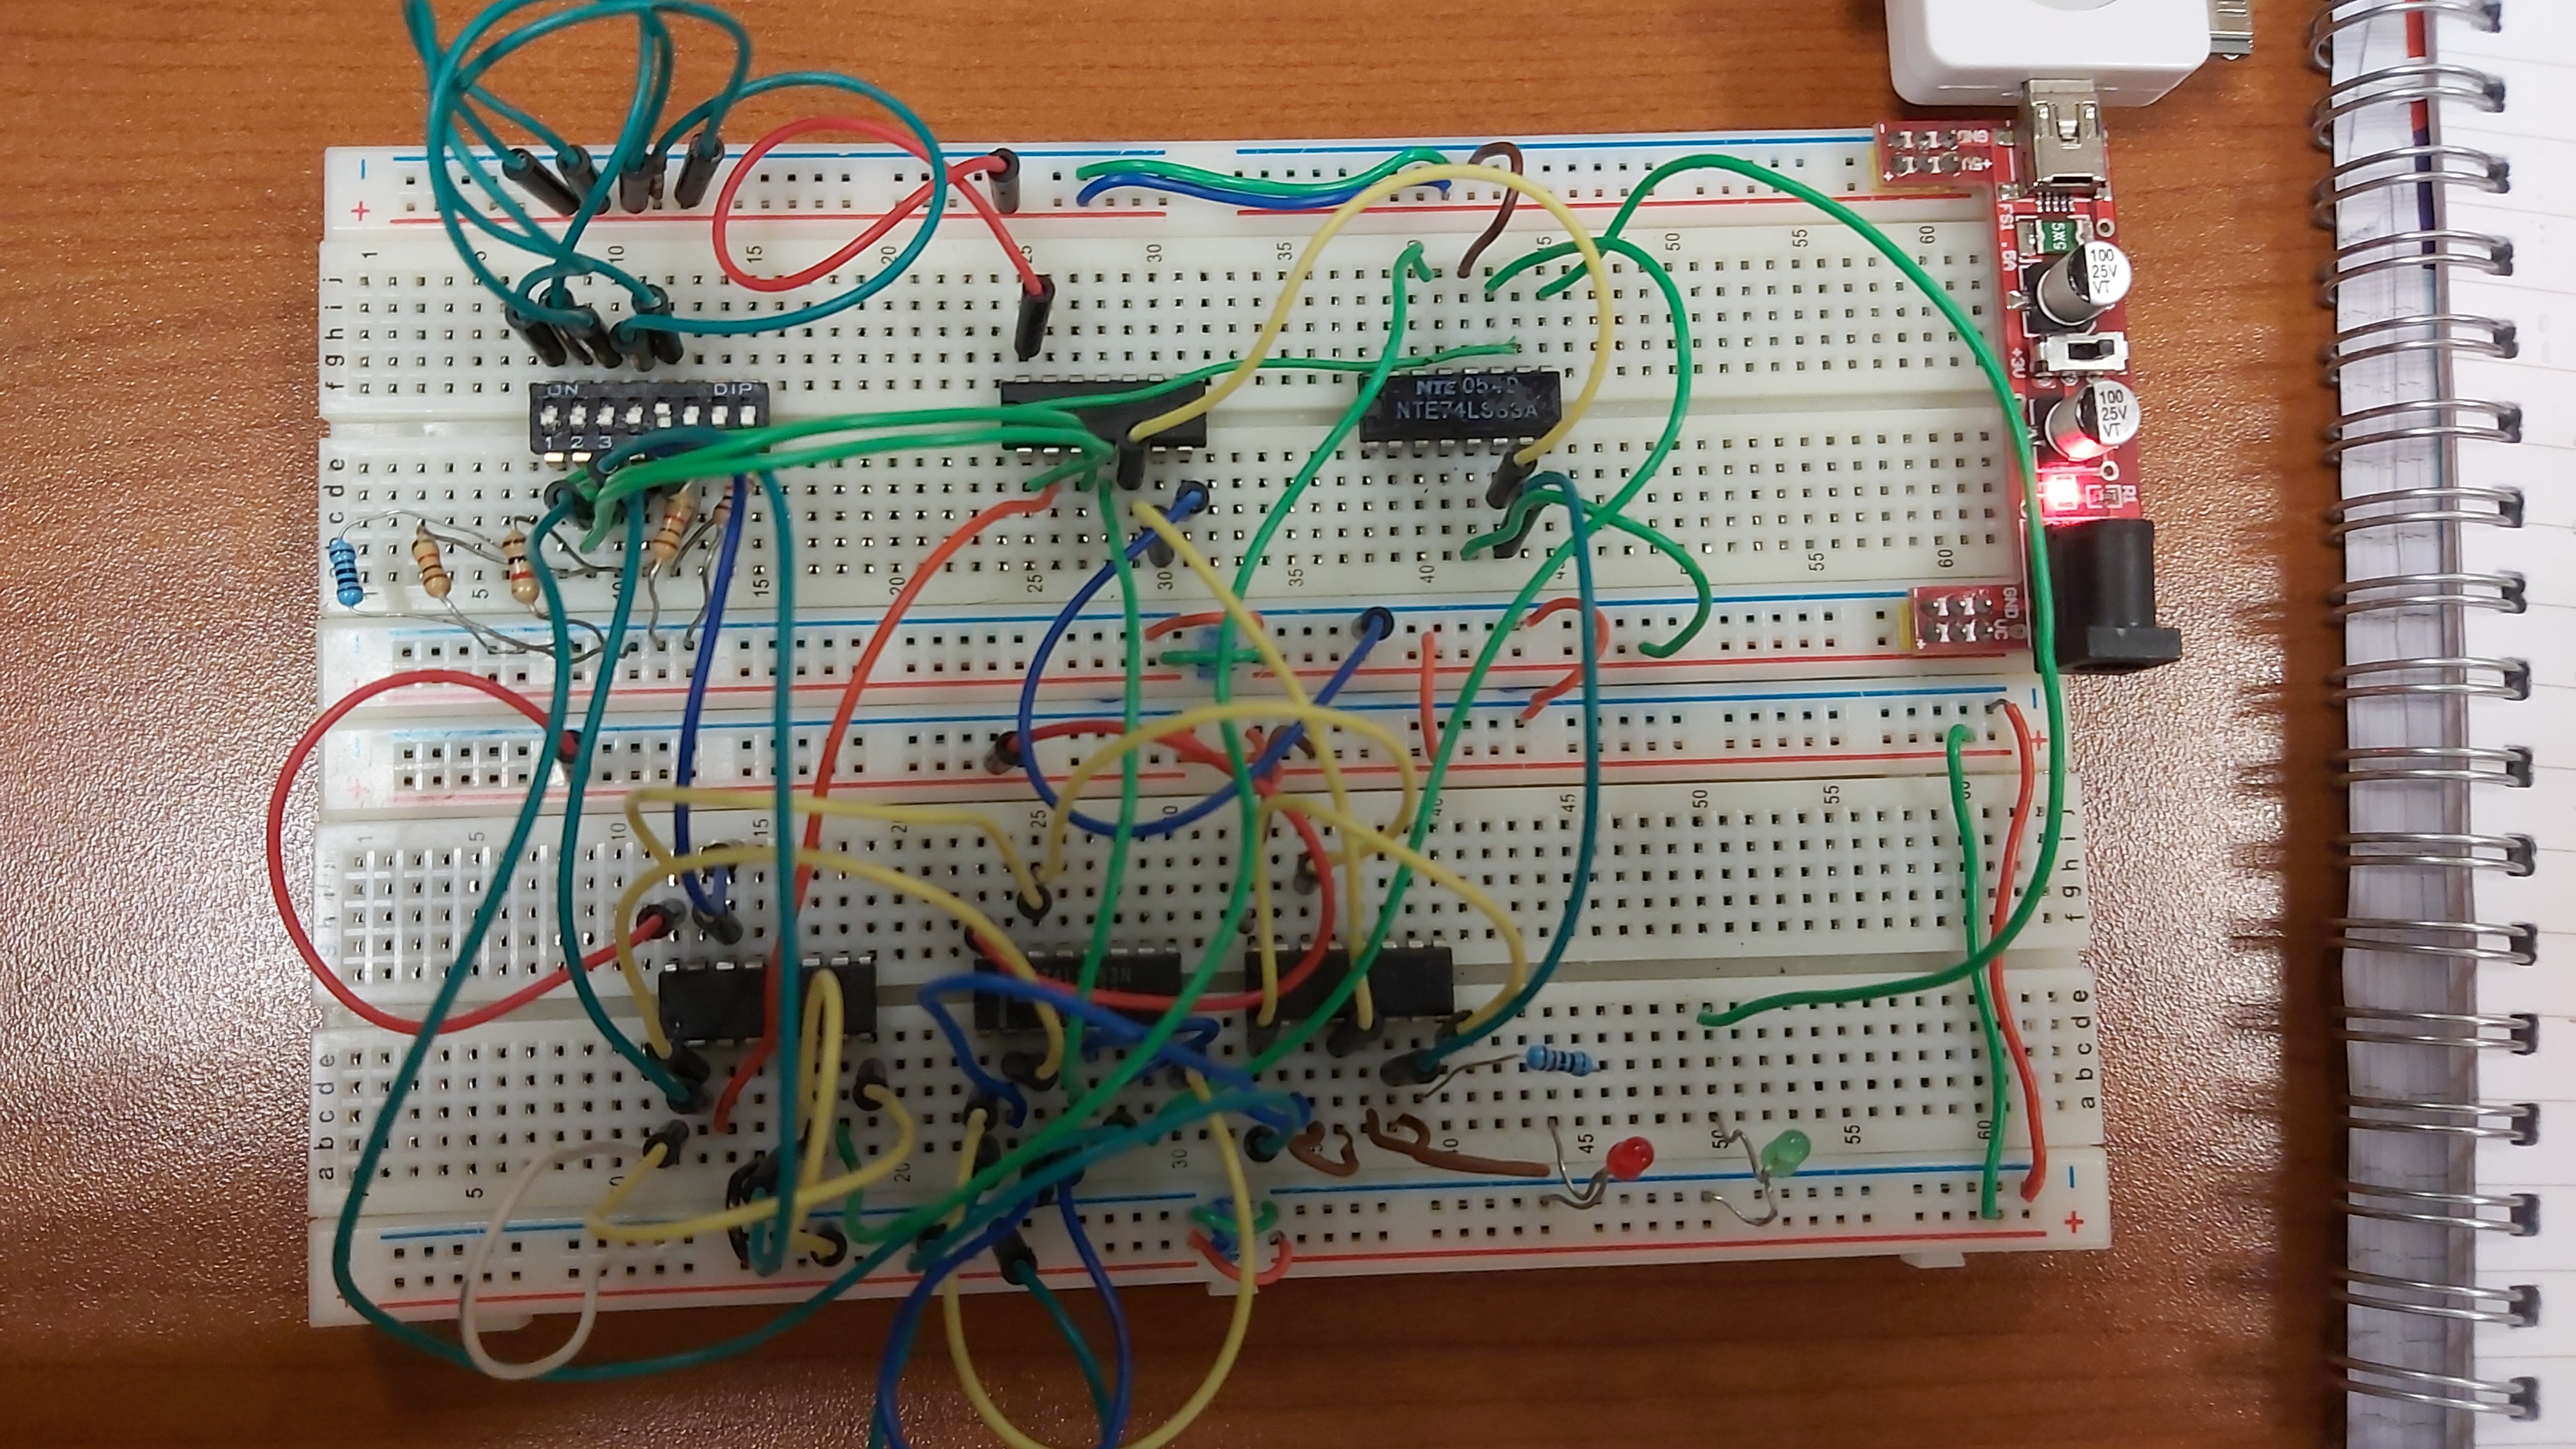
\includegraphics[width=\textwidth]{./figures/00001.jpg}
\begin{center}
	All inputs are off, and thus no LED is on.
\end{center}

\vspace{2em}

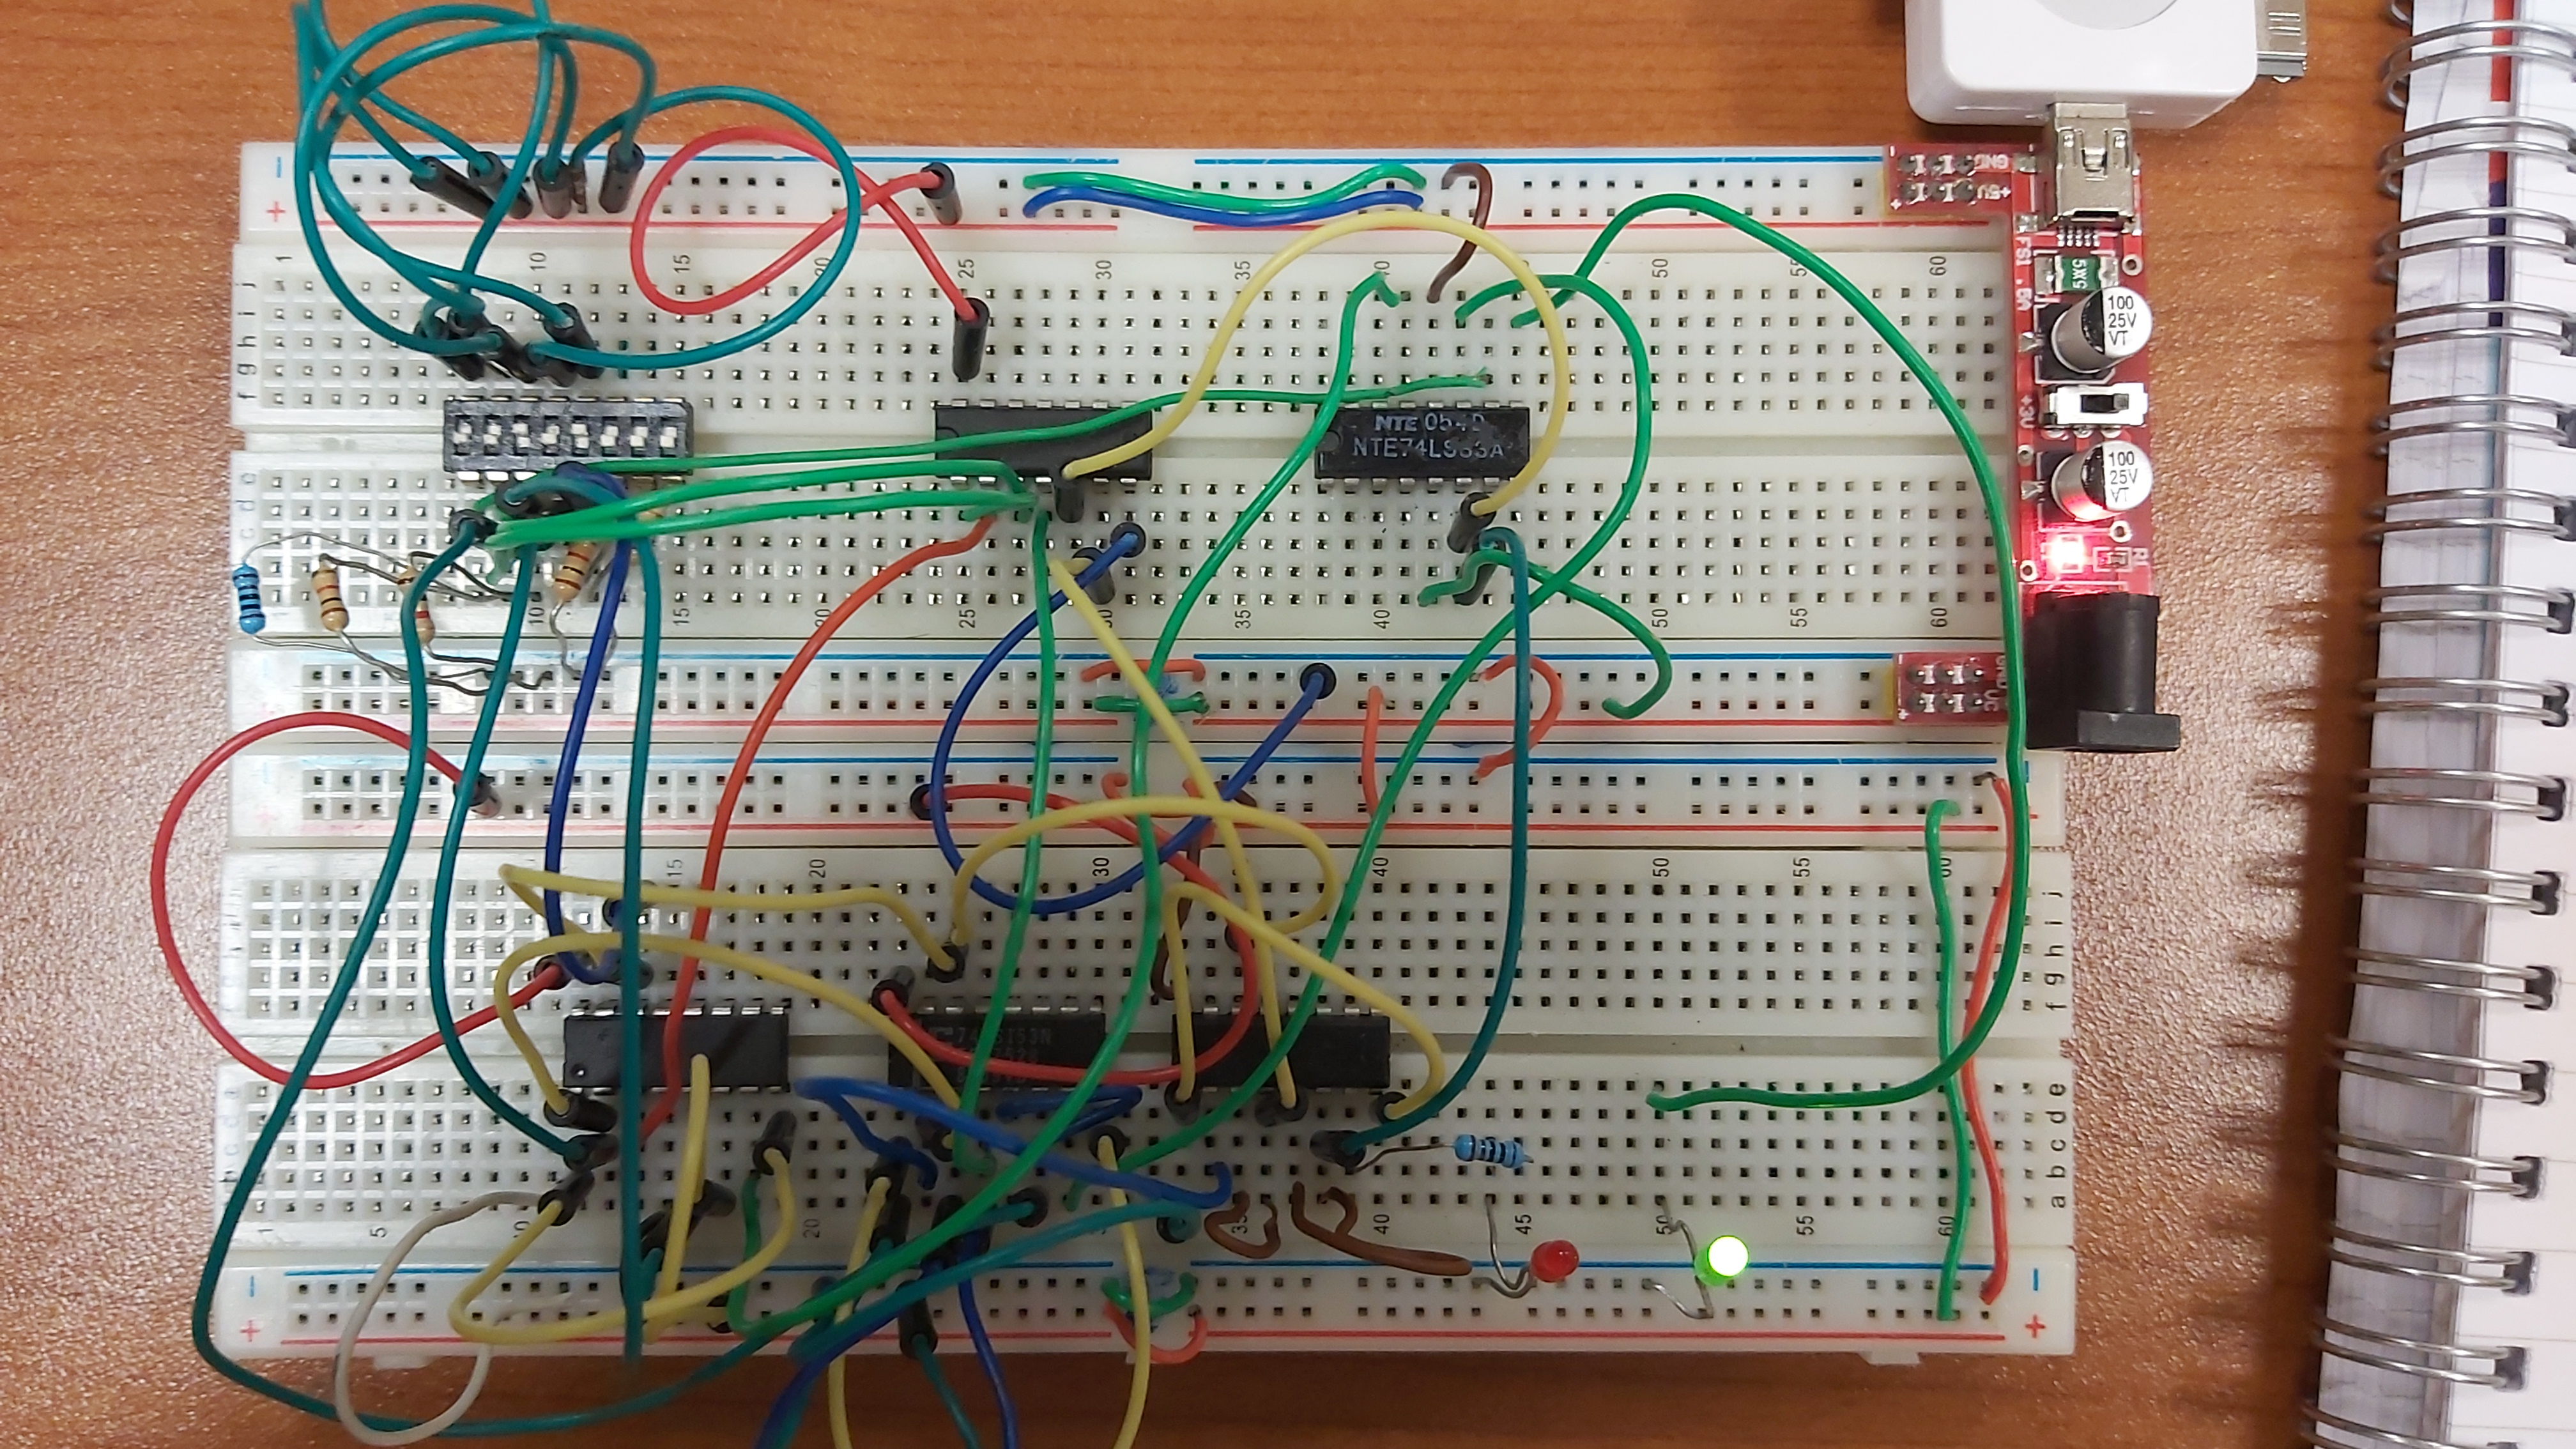
\includegraphics[width=\textwidth]{./figures/00101.jpg}
\begin{center}
	$ABC_i = 001$ and so $C_o Y= 01$.\\
\end{center}


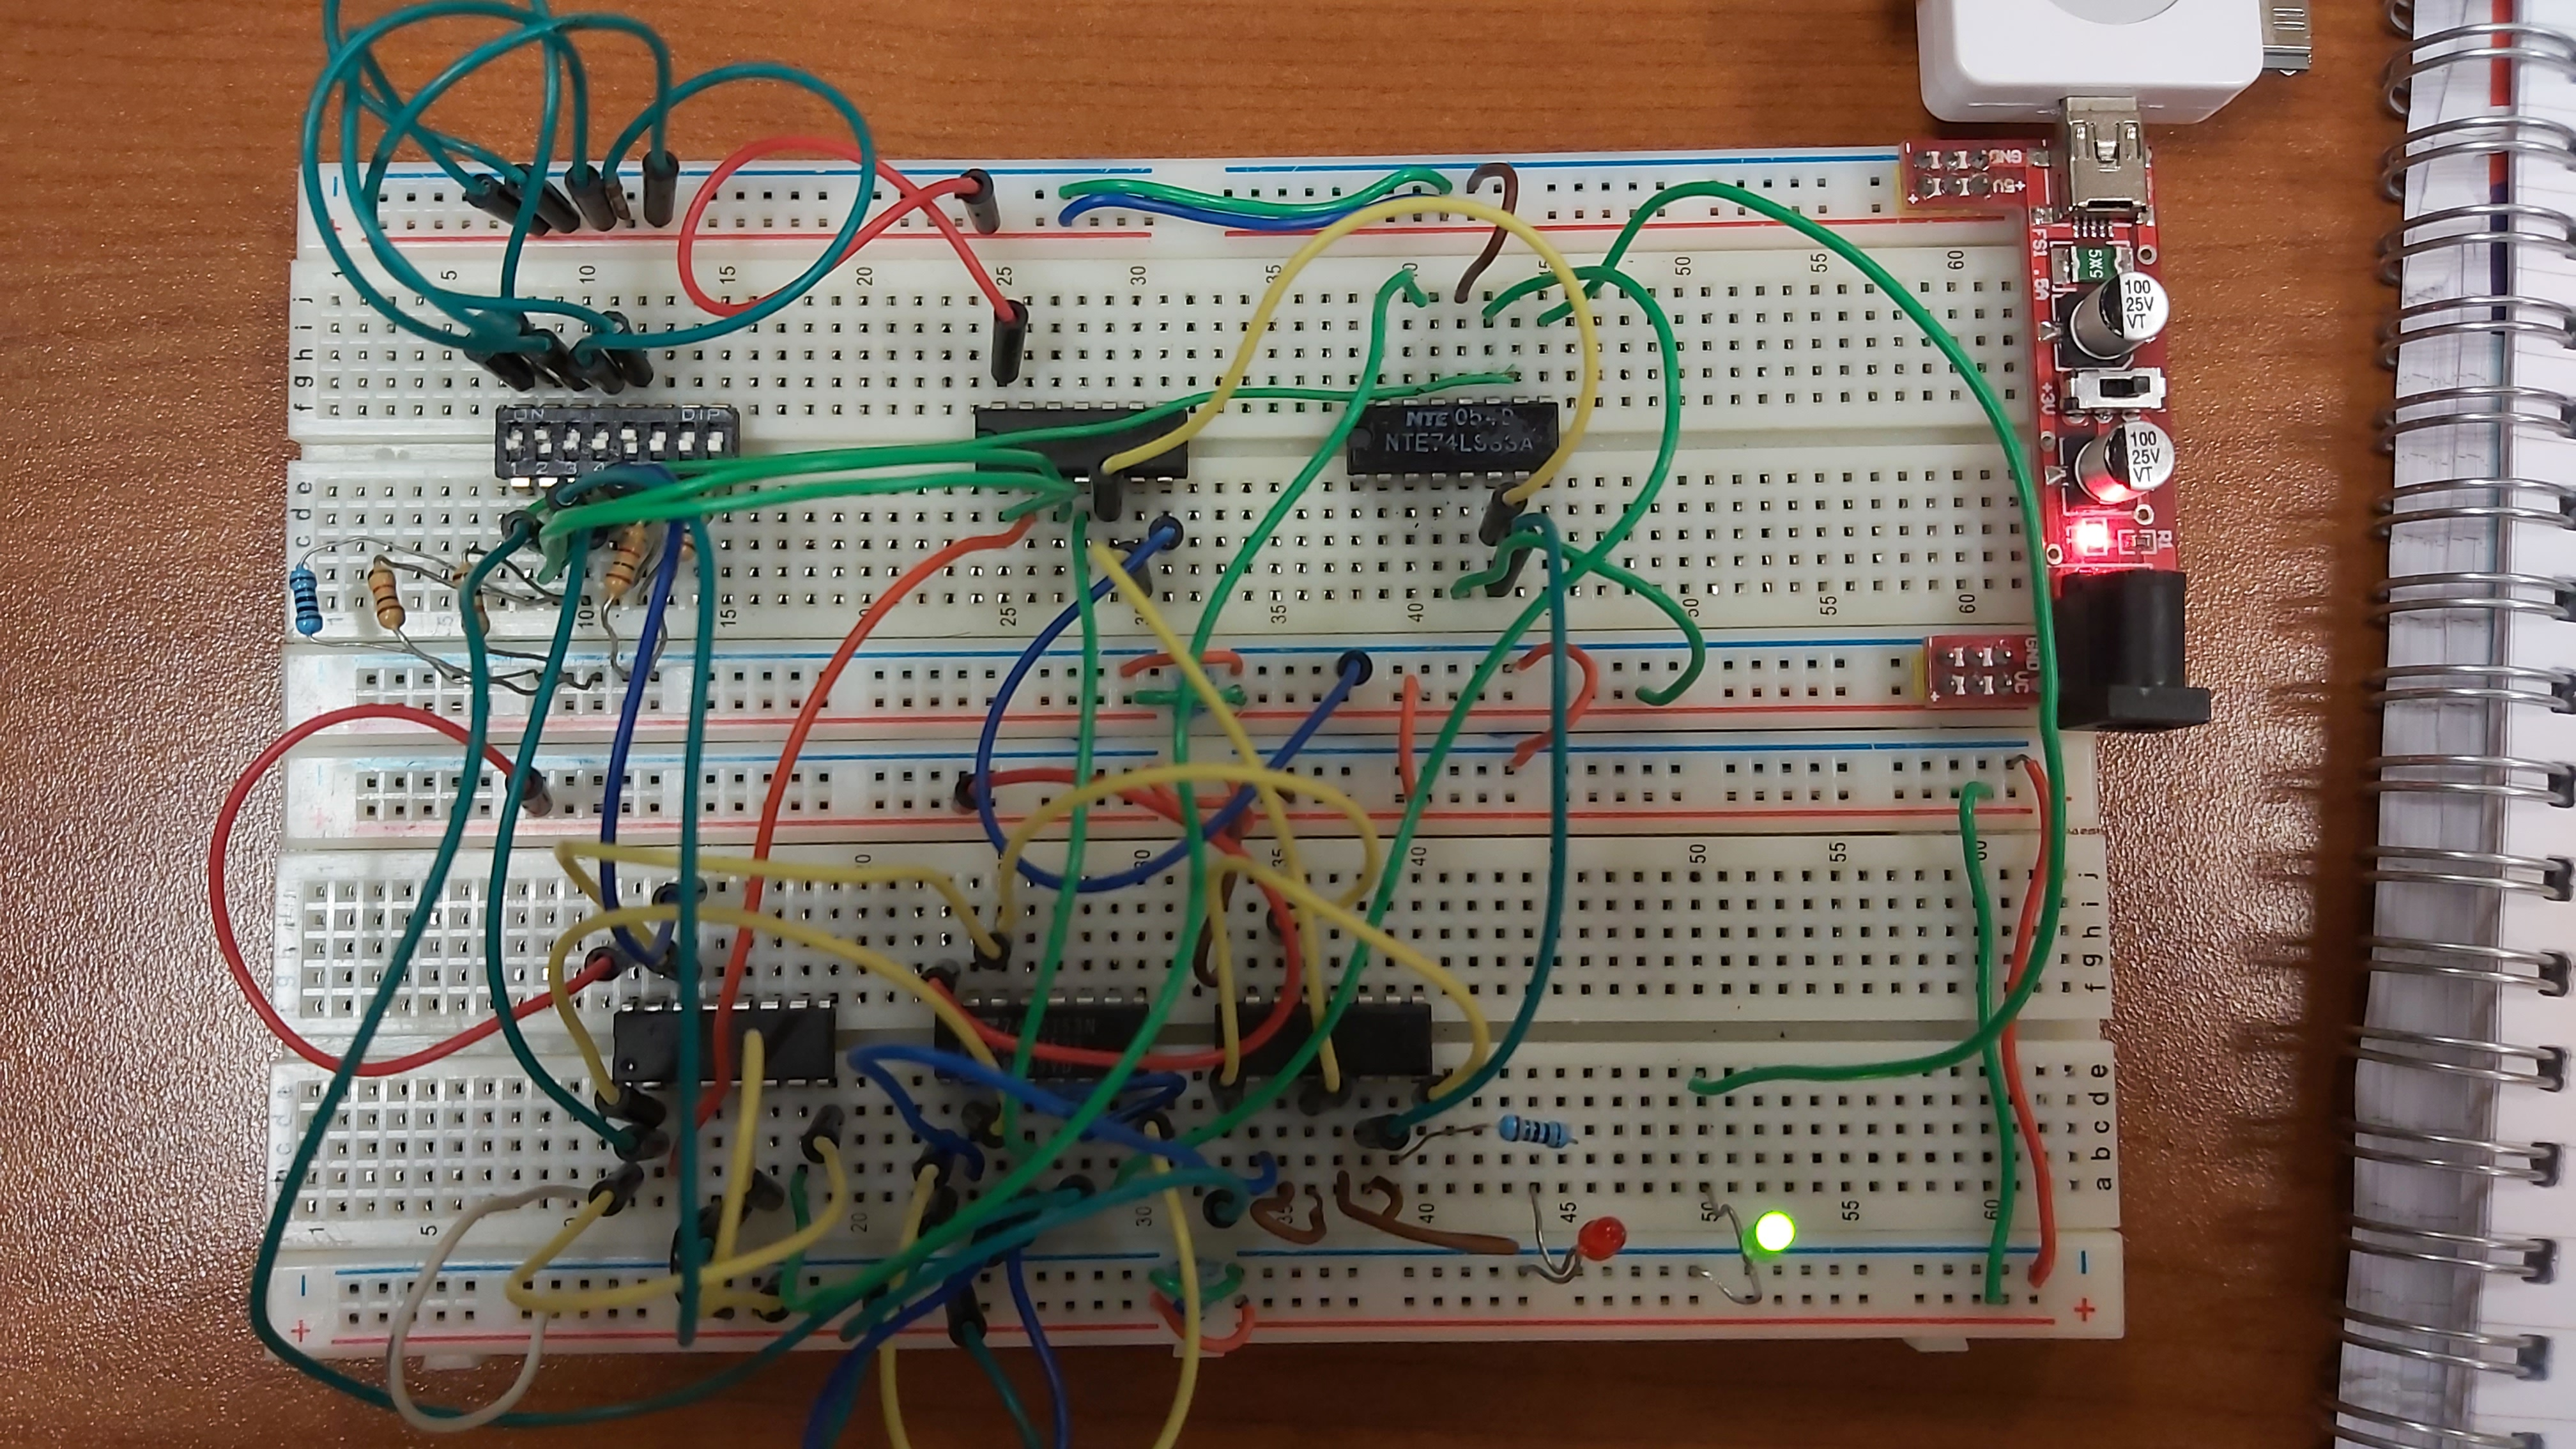
\includegraphics[width=\textwidth]{./figures/01001.jpg}
\begin{center}
	$ABC_i = 010$ and so $C_o Y= 01$.
\end{center}

\vspace{2em}

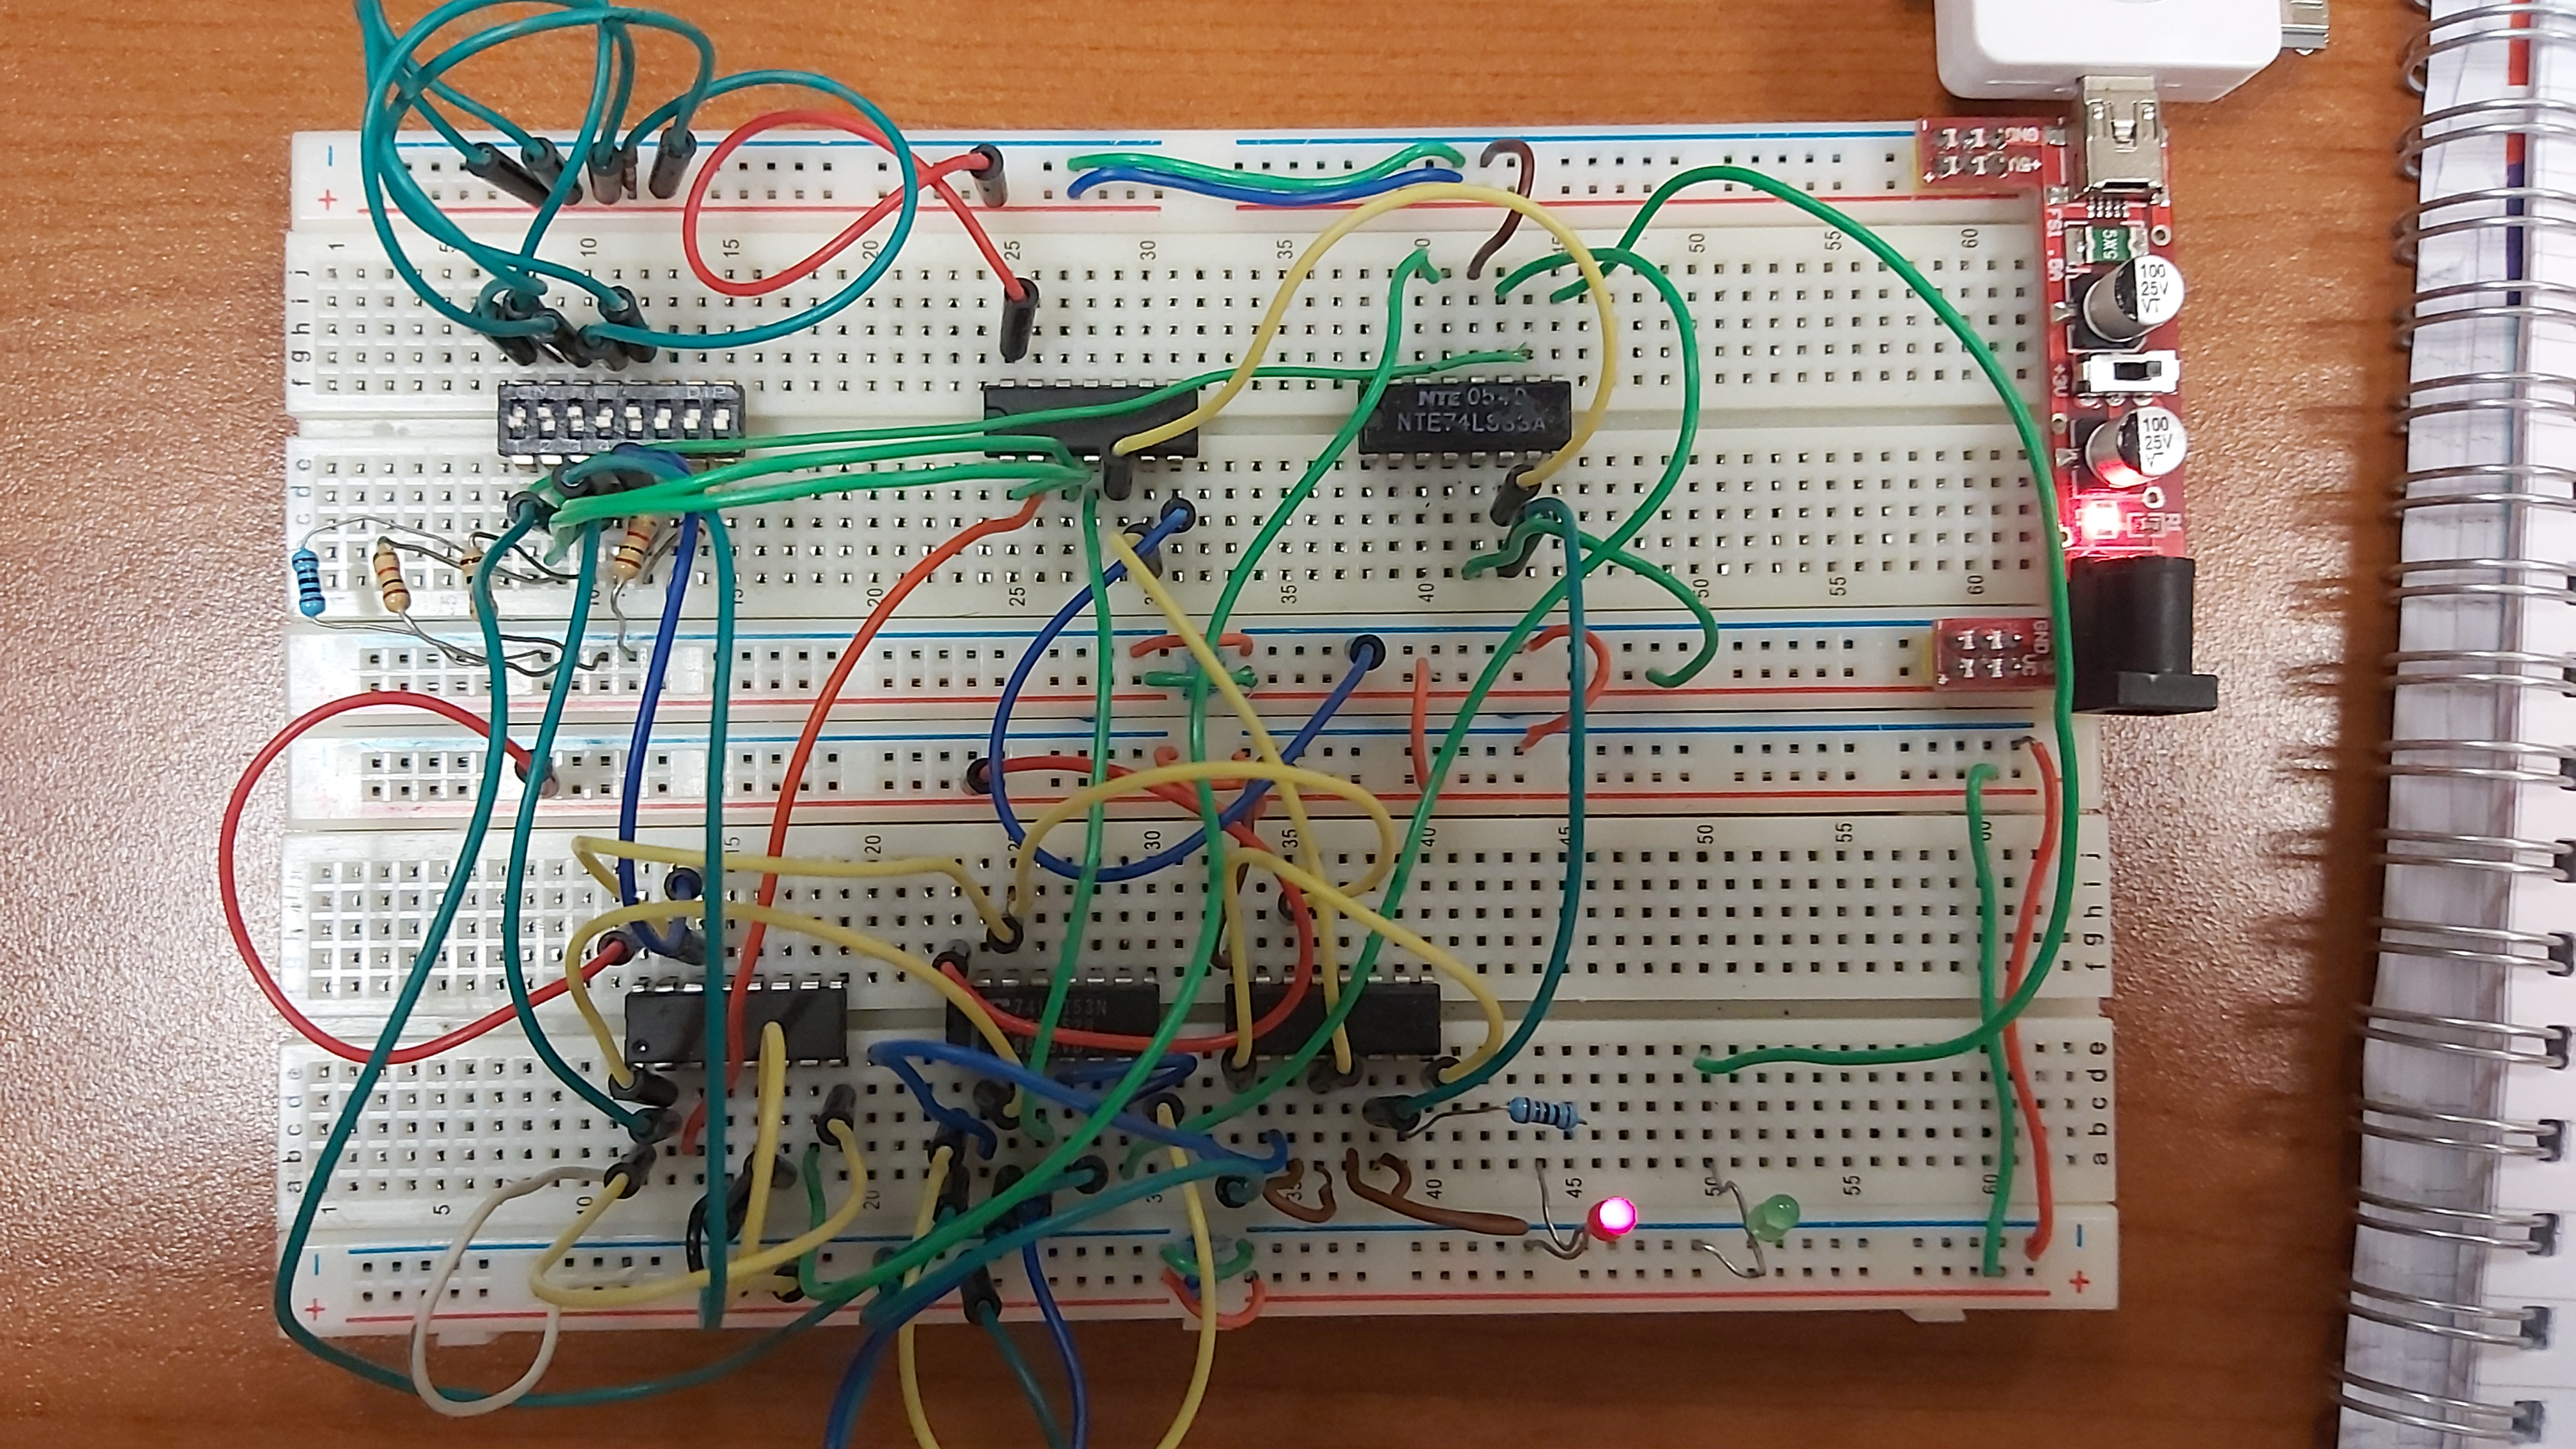
\includegraphics[width=\textwidth]{./figures/01101.jpg}
\begin{center}
	$ABC_i = 011$ and so $C_o Y= 10$.
\end{center}


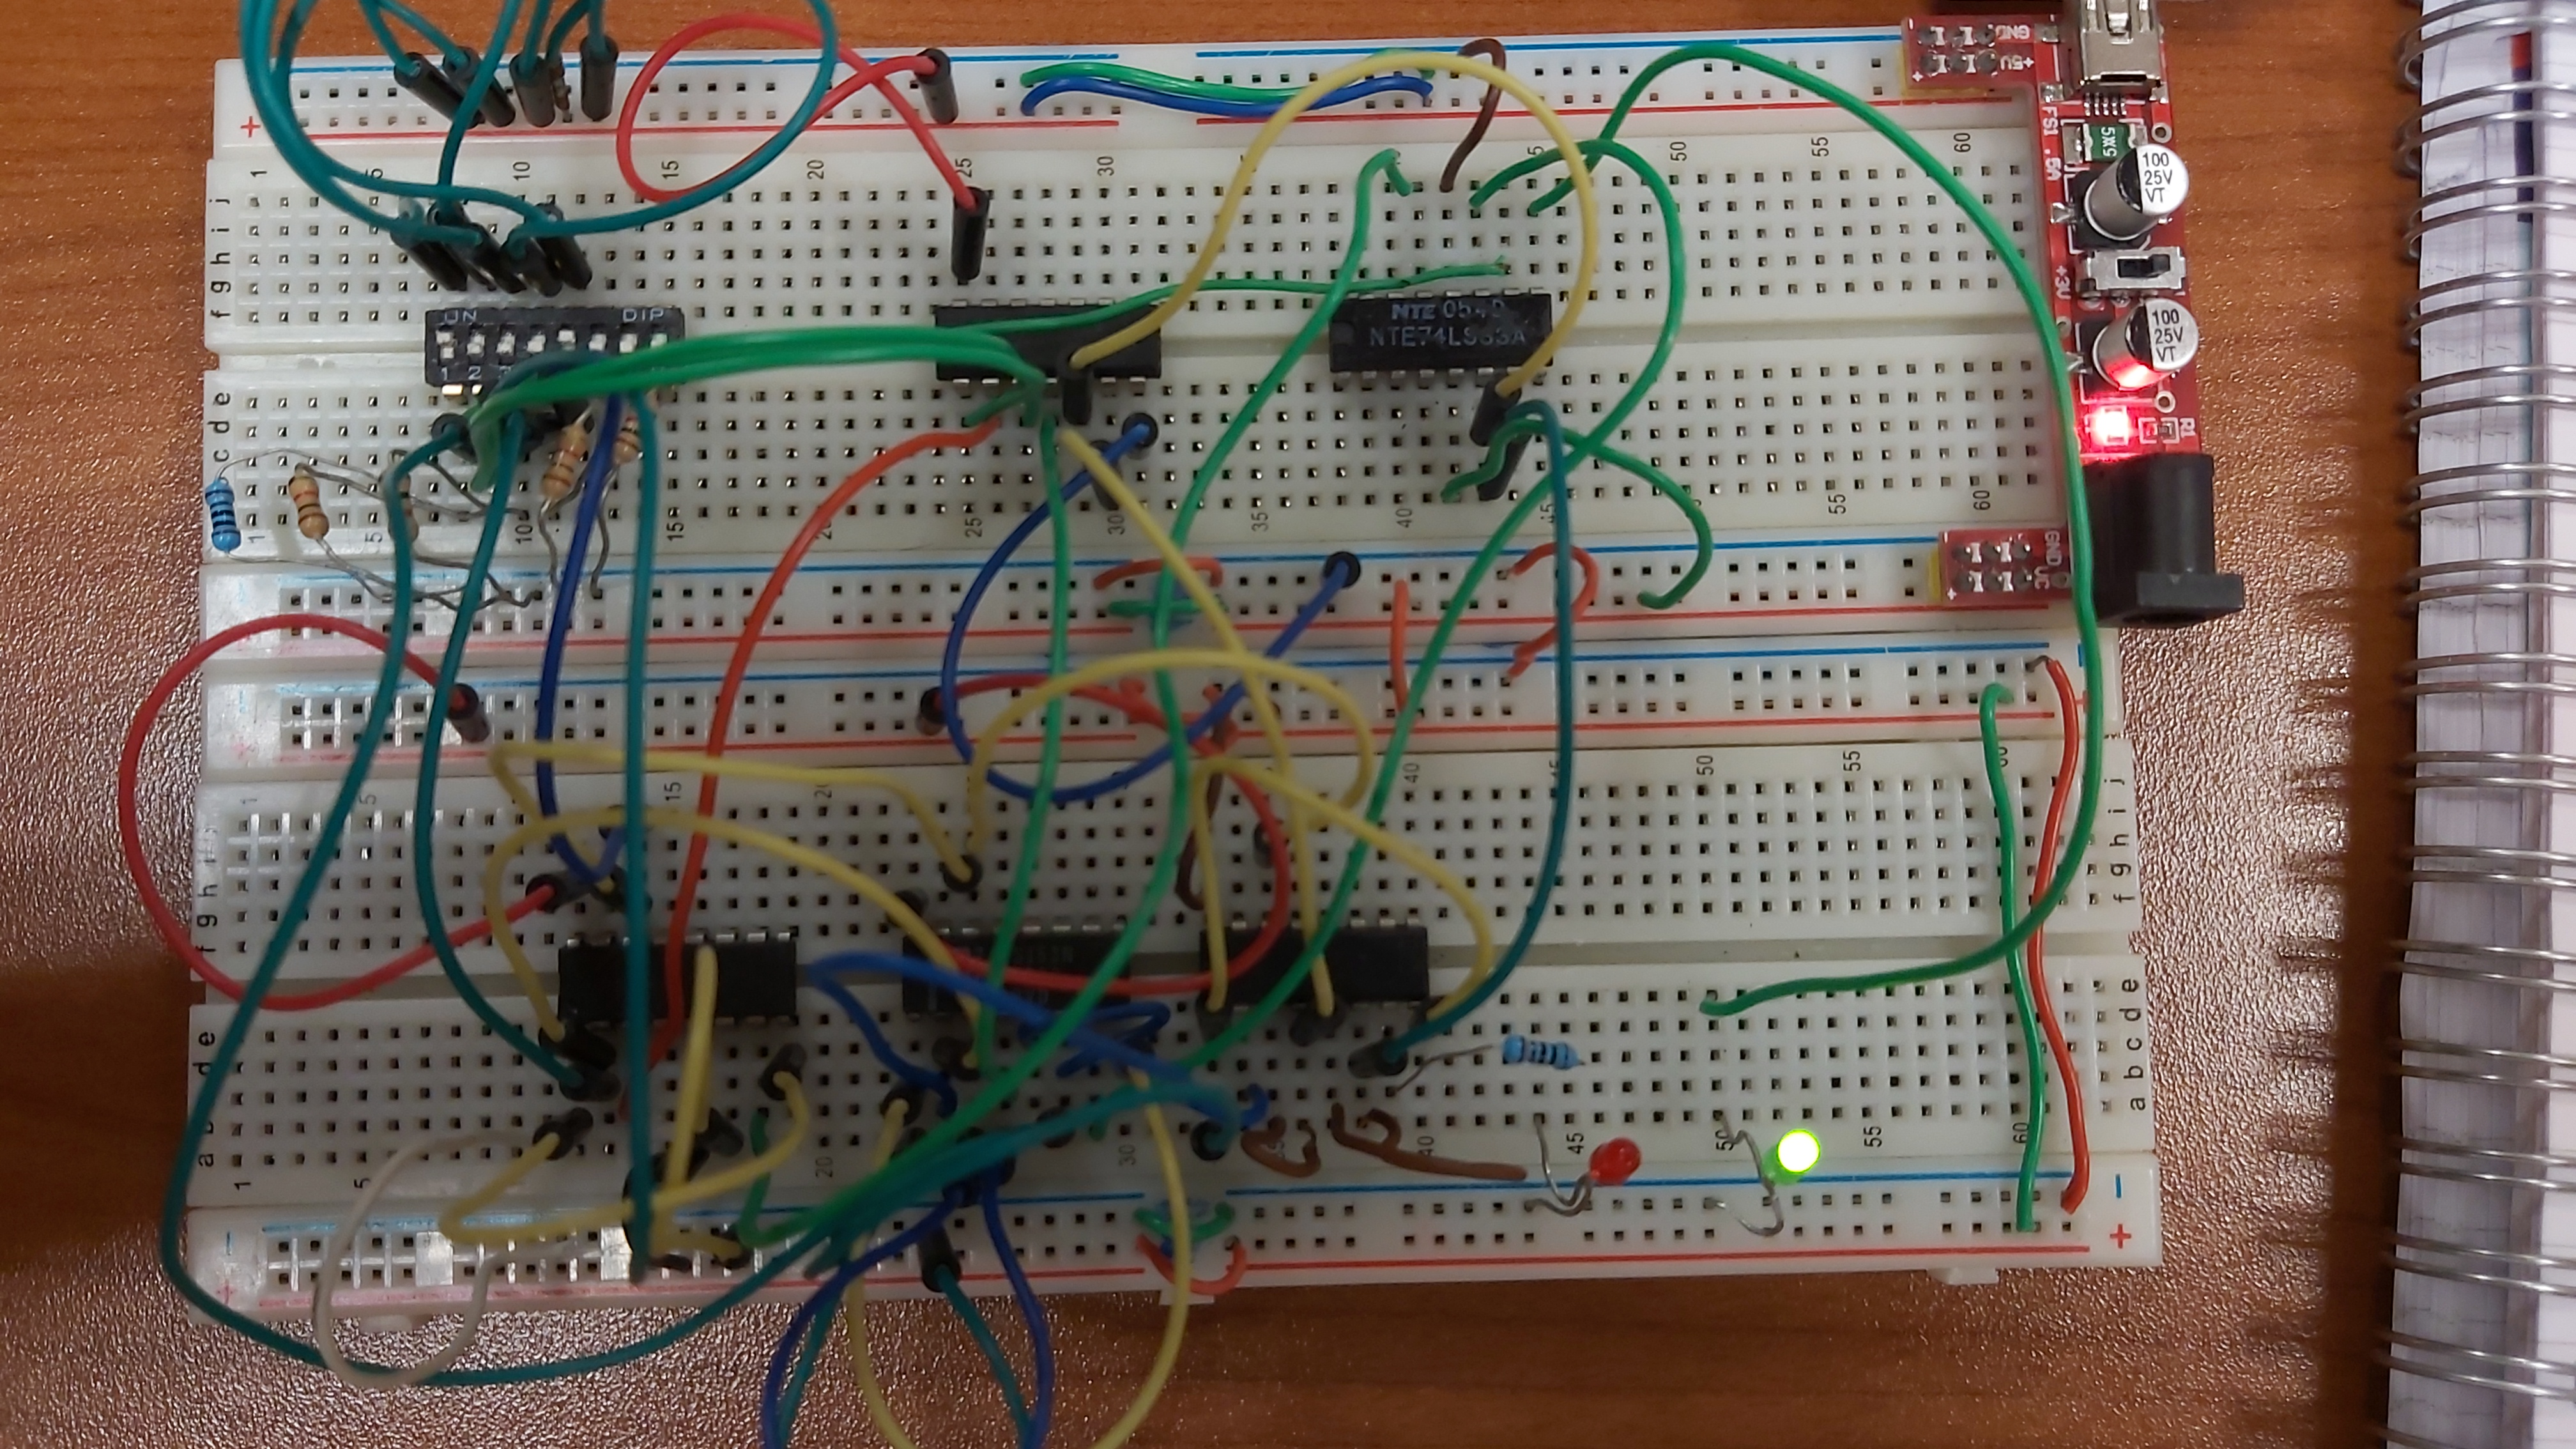
\includegraphics[width=\textwidth]{./figures/10001.jpg}
\begin{center}
	$ABC_i = 100$ and so $C_o Y= 01$.
\end{center}

\vspace{2em}

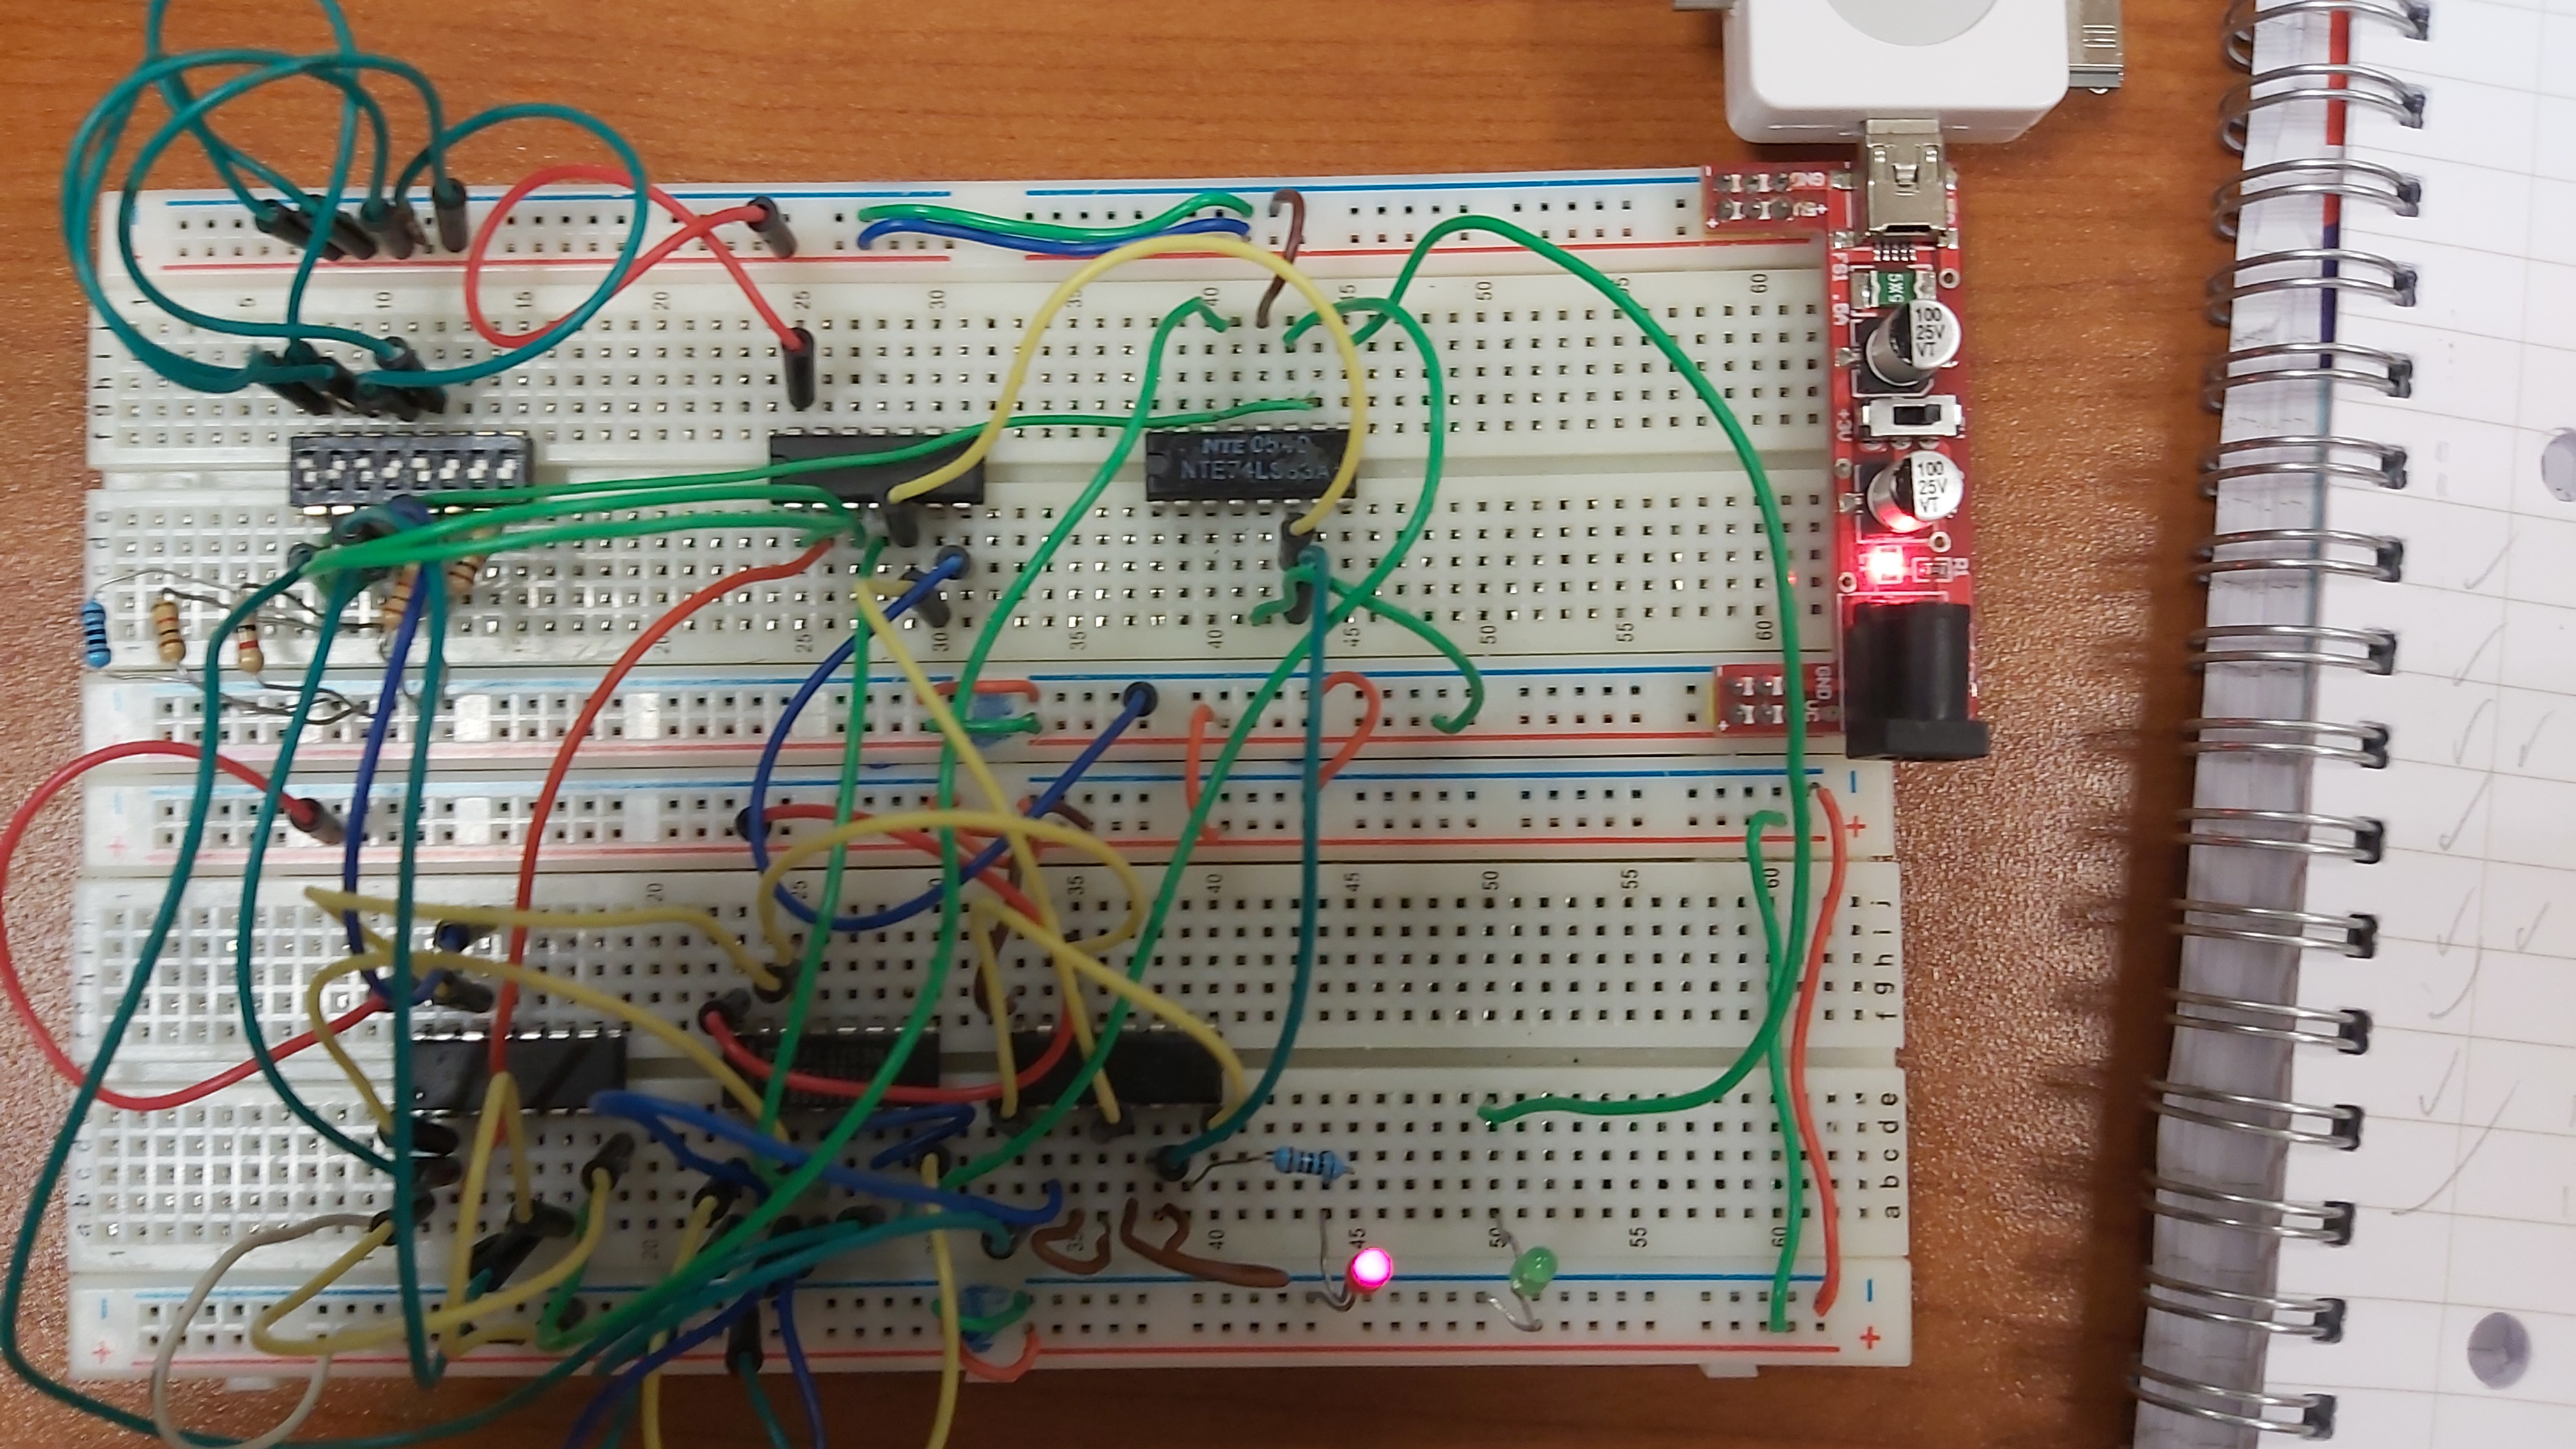
\includegraphics[width=\textwidth]{./figures/10101.jpg}
\begin{center}
	$ABC_i = 101$ and so $C_o Y= 10$.
\end{center}


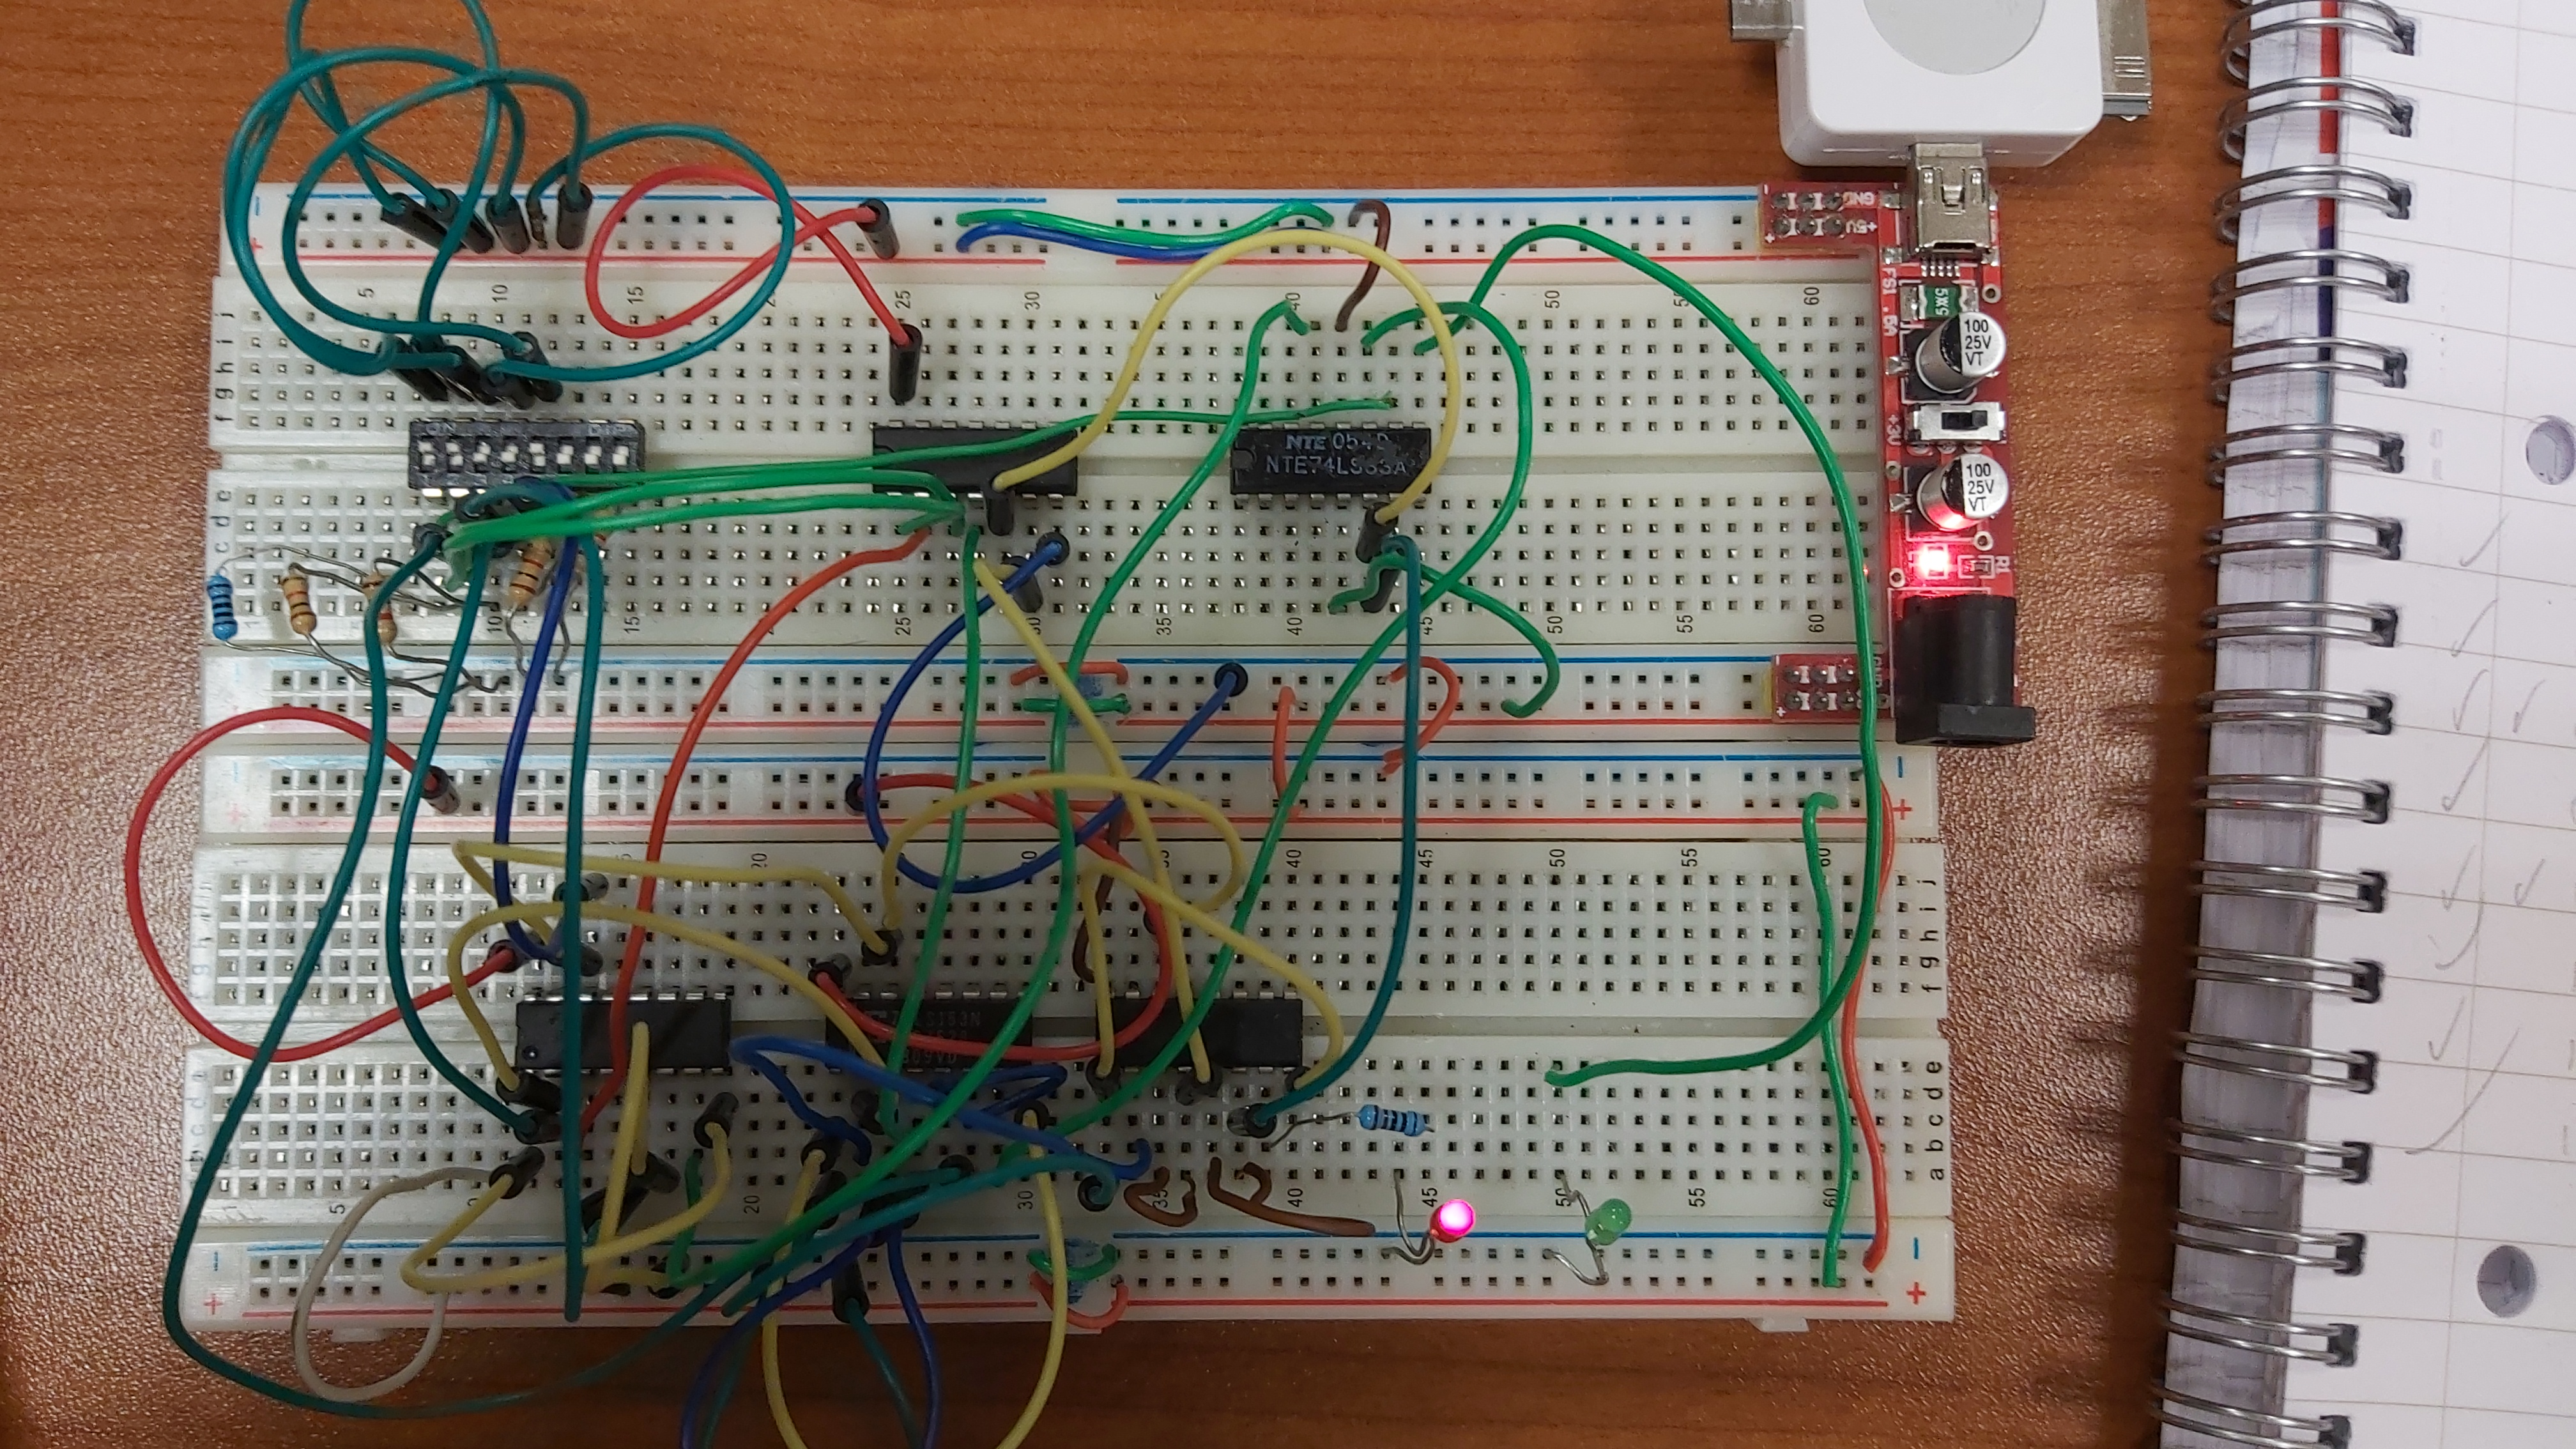
\includegraphics[width=\textwidth]{./figures/11001.jpg}
\begin{center}
	$ABC_i = 110$ and so $C_o Y= 10$.
\end{center}

\vspace{2em}

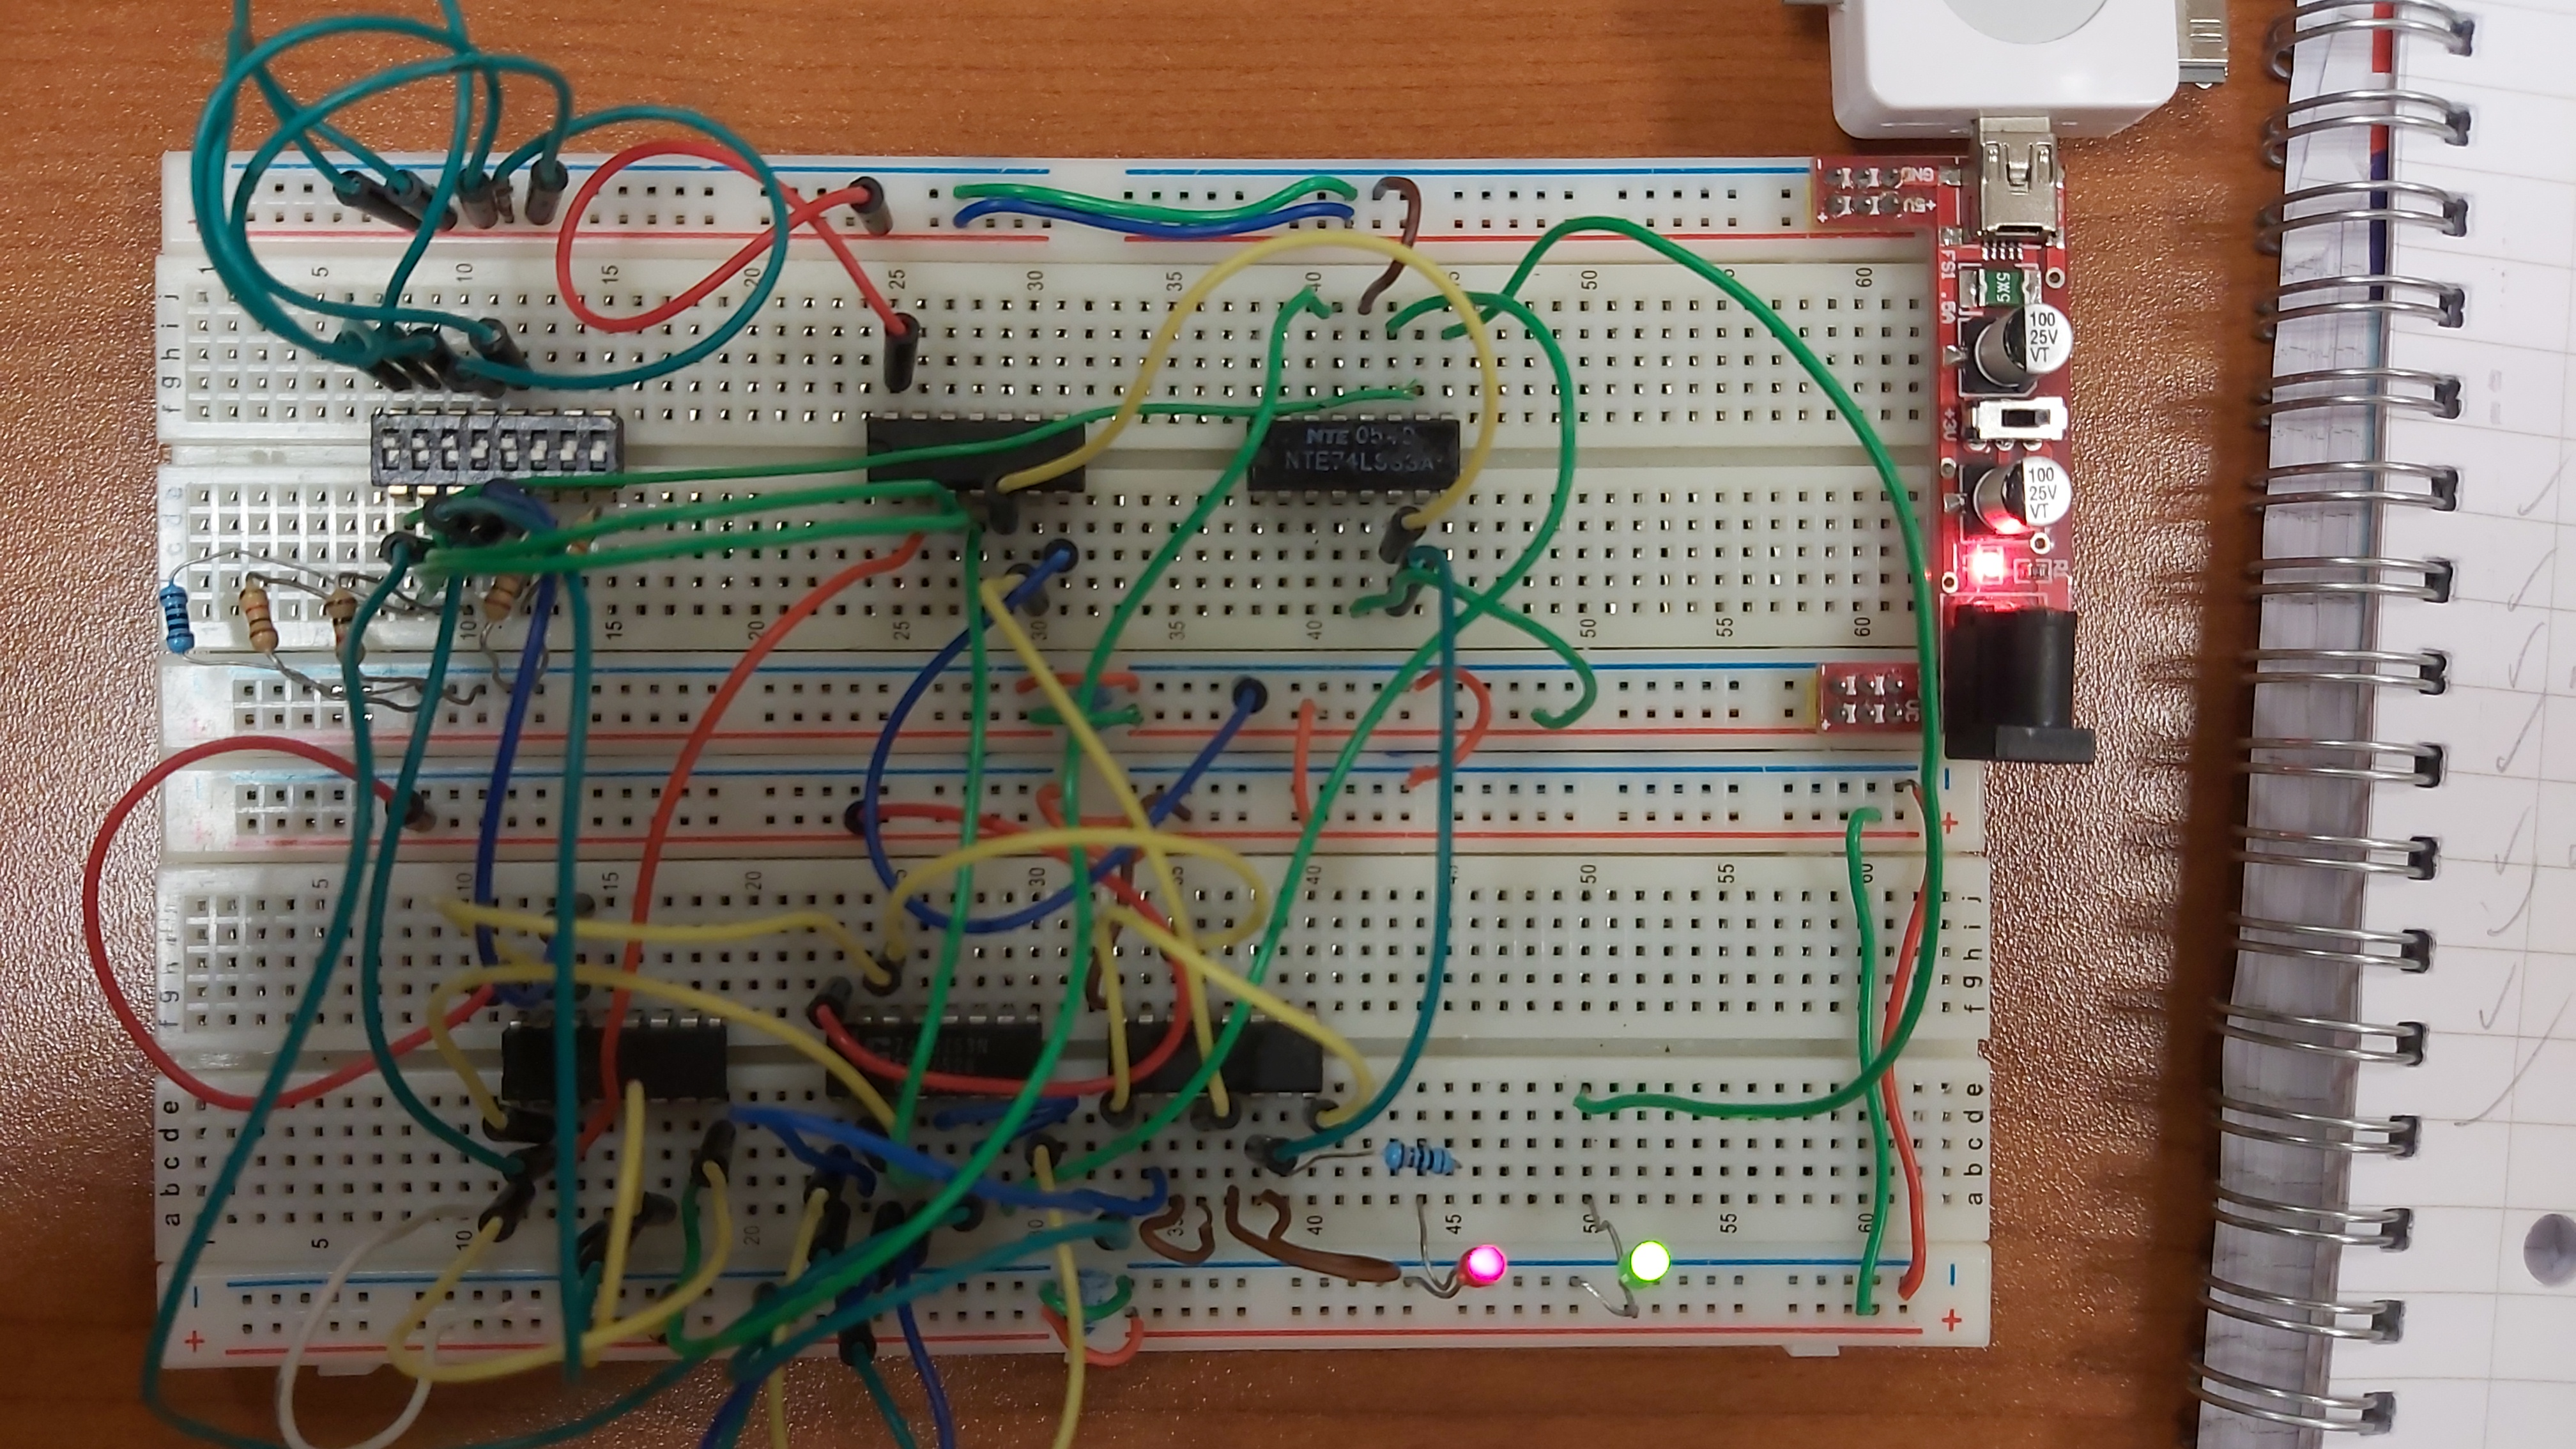
\includegraphics[width=\textwidth]{./figures/11101.jpg}
\begin{center}
	$ABC_i = 111$ and so $C_o Y= 11$.
\end{center}

\subsection{Opcode \texttt{10 - SUB}}

With this opcode selected, the ALU performs the subtraction of bits $A$ and $B$, or rather, the
addition of $A$, $\bar{B}$ and 1, whilst ignoring the borrow bit $C_{i}$. When a negative value is
obtained, the resultant representation will be one in 2's complement, and so $-1_{10}$ would be
represented as $11_2 = -2_10 + 1_10$.

\[A+\bar{B}+1 = C_o Y\]

\vspace{9em}

\subsubsection{Truth table}

\begin{center}
	\Large
	\begin{tabular}{c|c|c||c|c||c|c|c}
		$A$ & $B$ & $C_i$ & $Op_1$ & $Op_2$ & $C_{o}$ & $Y$ \\
		\hline
		0 & 0 & 0 & 1 & 0 & 0 & 0 \\
		0 & 0 & 1 & 1 & 0 & 0 & 0 \\
		0 & 1 & 0 & 1 & 0 & 1 & 1 \\
		0 & 1 & 1 & 1 & 0 & 0 & 0 \\
		1 & 0 & 0 & 1 & 0 & 0 & 1 \\
		1 & 0 & 1 & 1 & 0 & 0 & 1 \\
		1 & 1 & 0 & 1 & 0 & 0 & 0 \\
		1 & 1 & 1 & 1 & 0 & 0 & 0 \\
	\end{tabular}
\end{center}


\newpage

\subsubsection{Pictures}


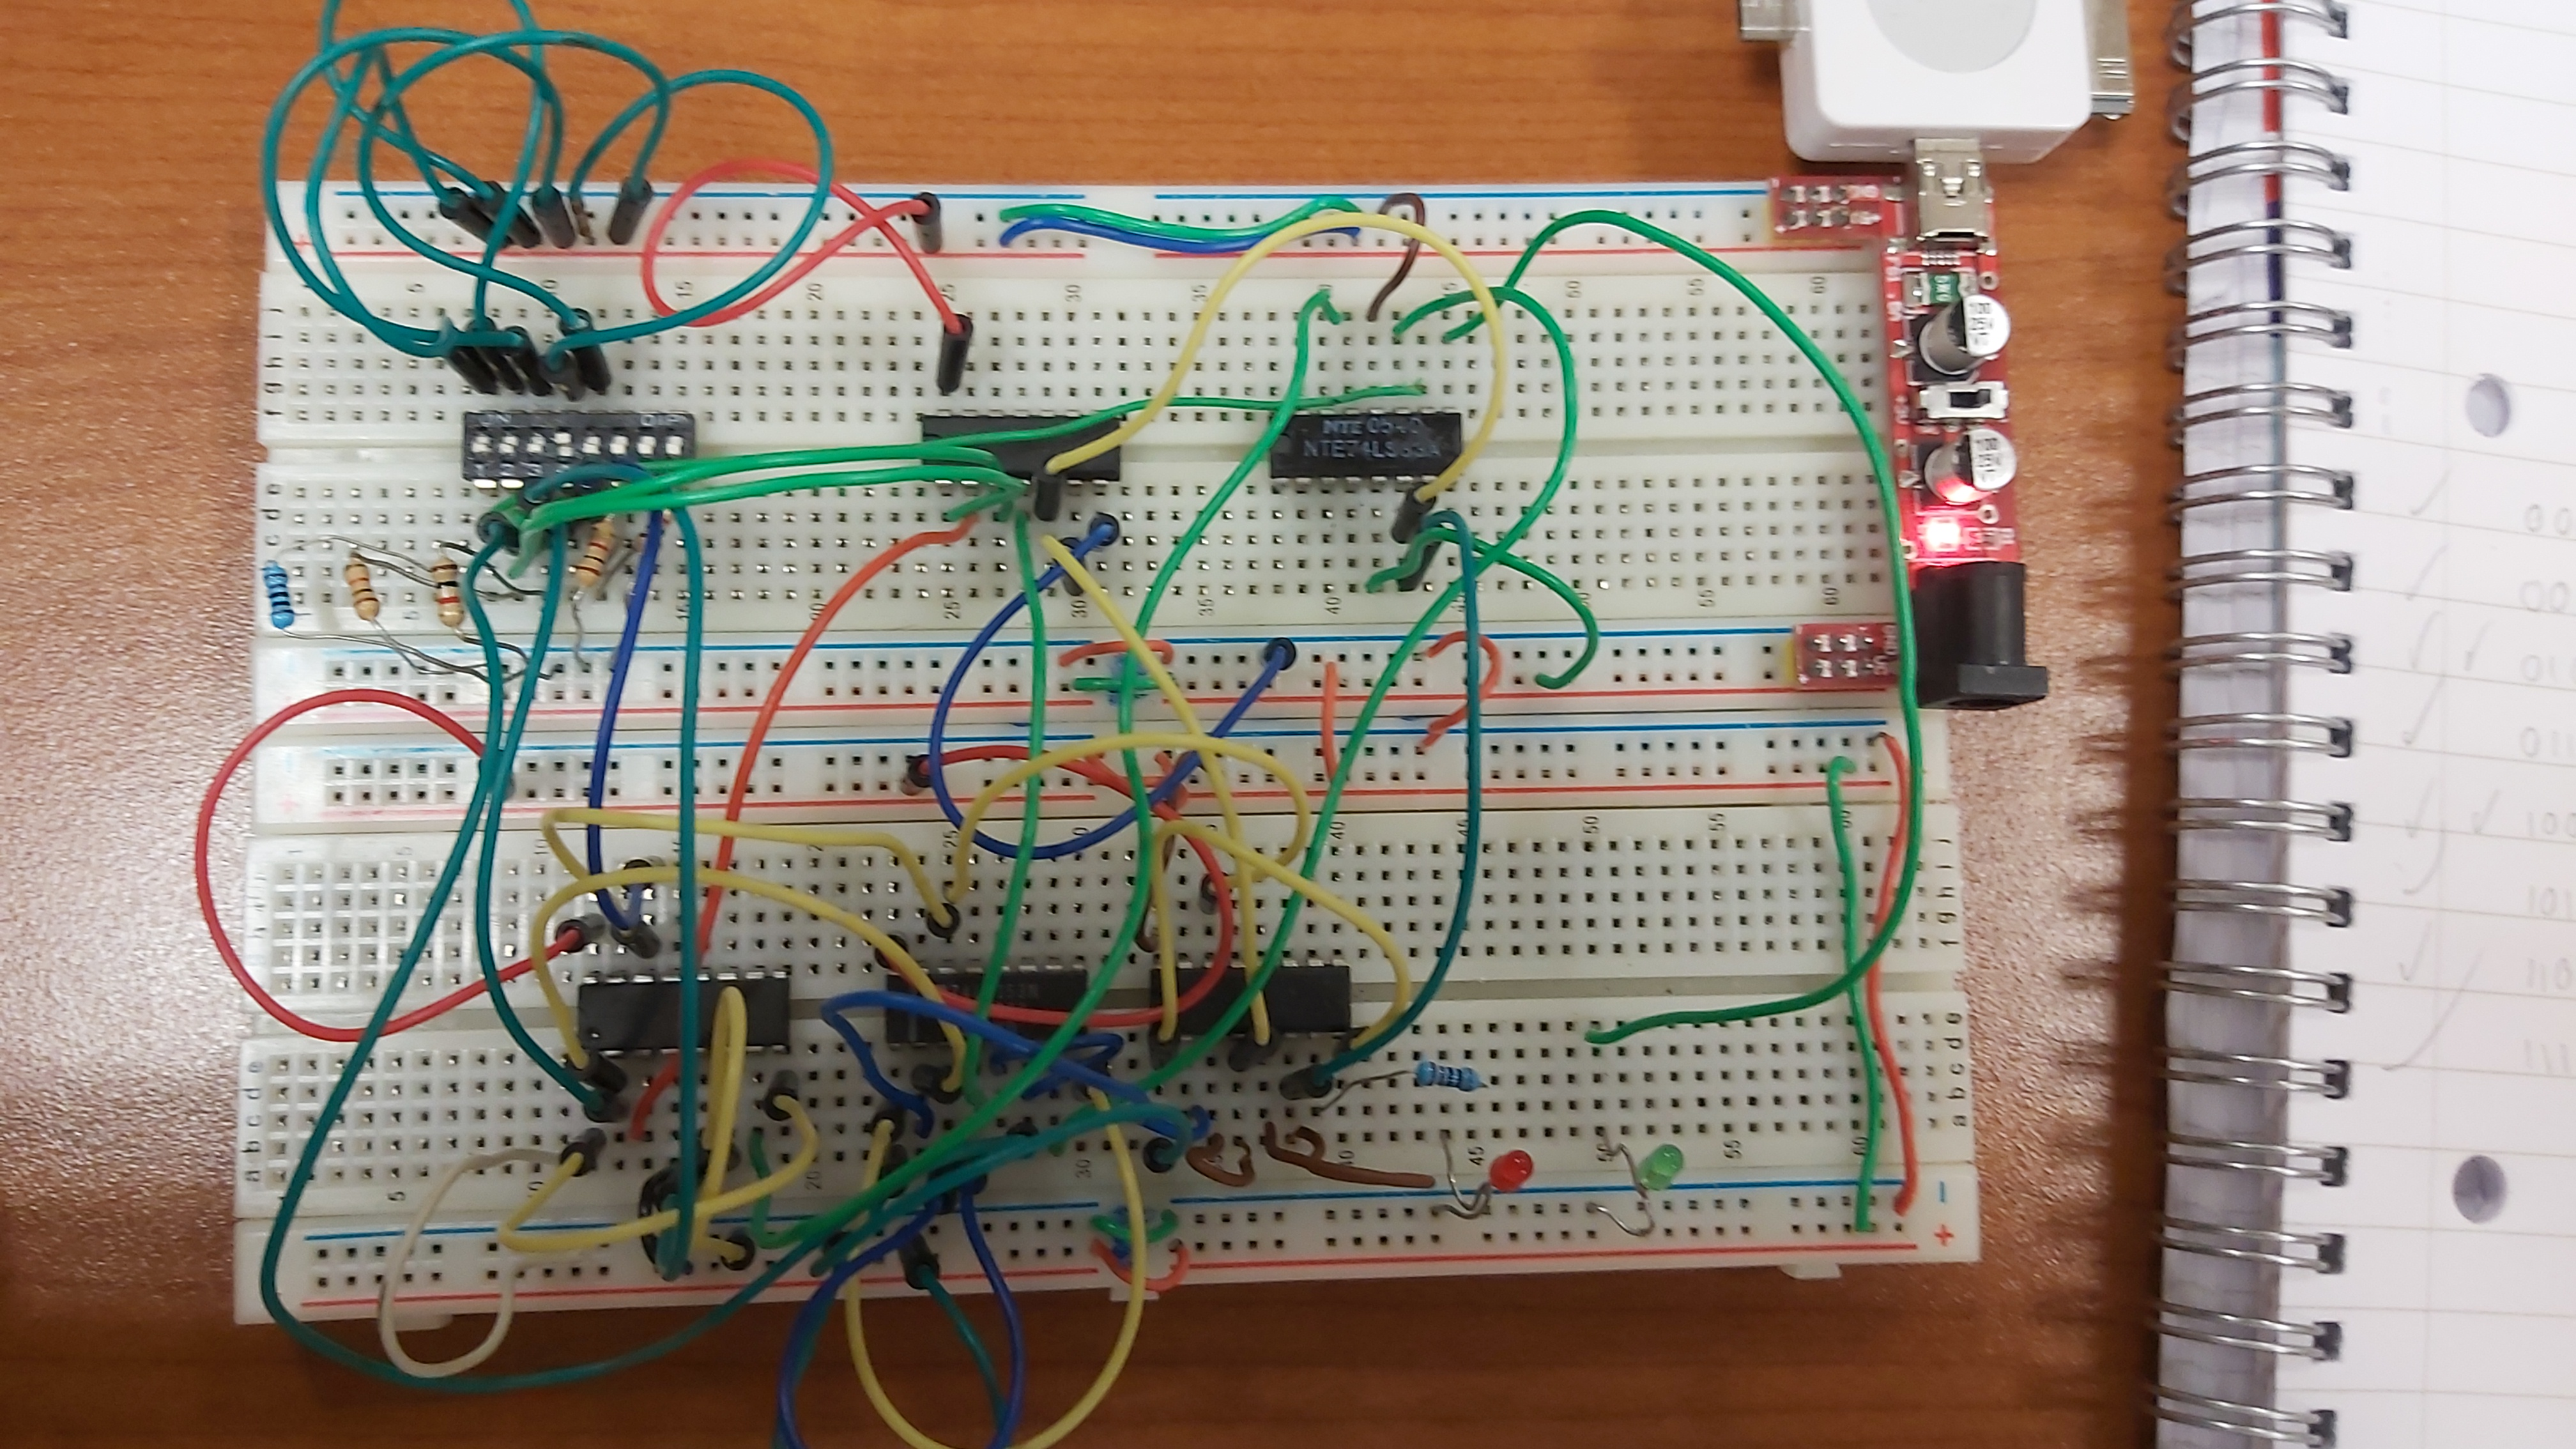
\includegraphics[width=\textwidth]{./figures/00010.jpg}
\begin{center}
	All inputs are off, and thus no LED is on.
\end{center}

\vspace{2em}

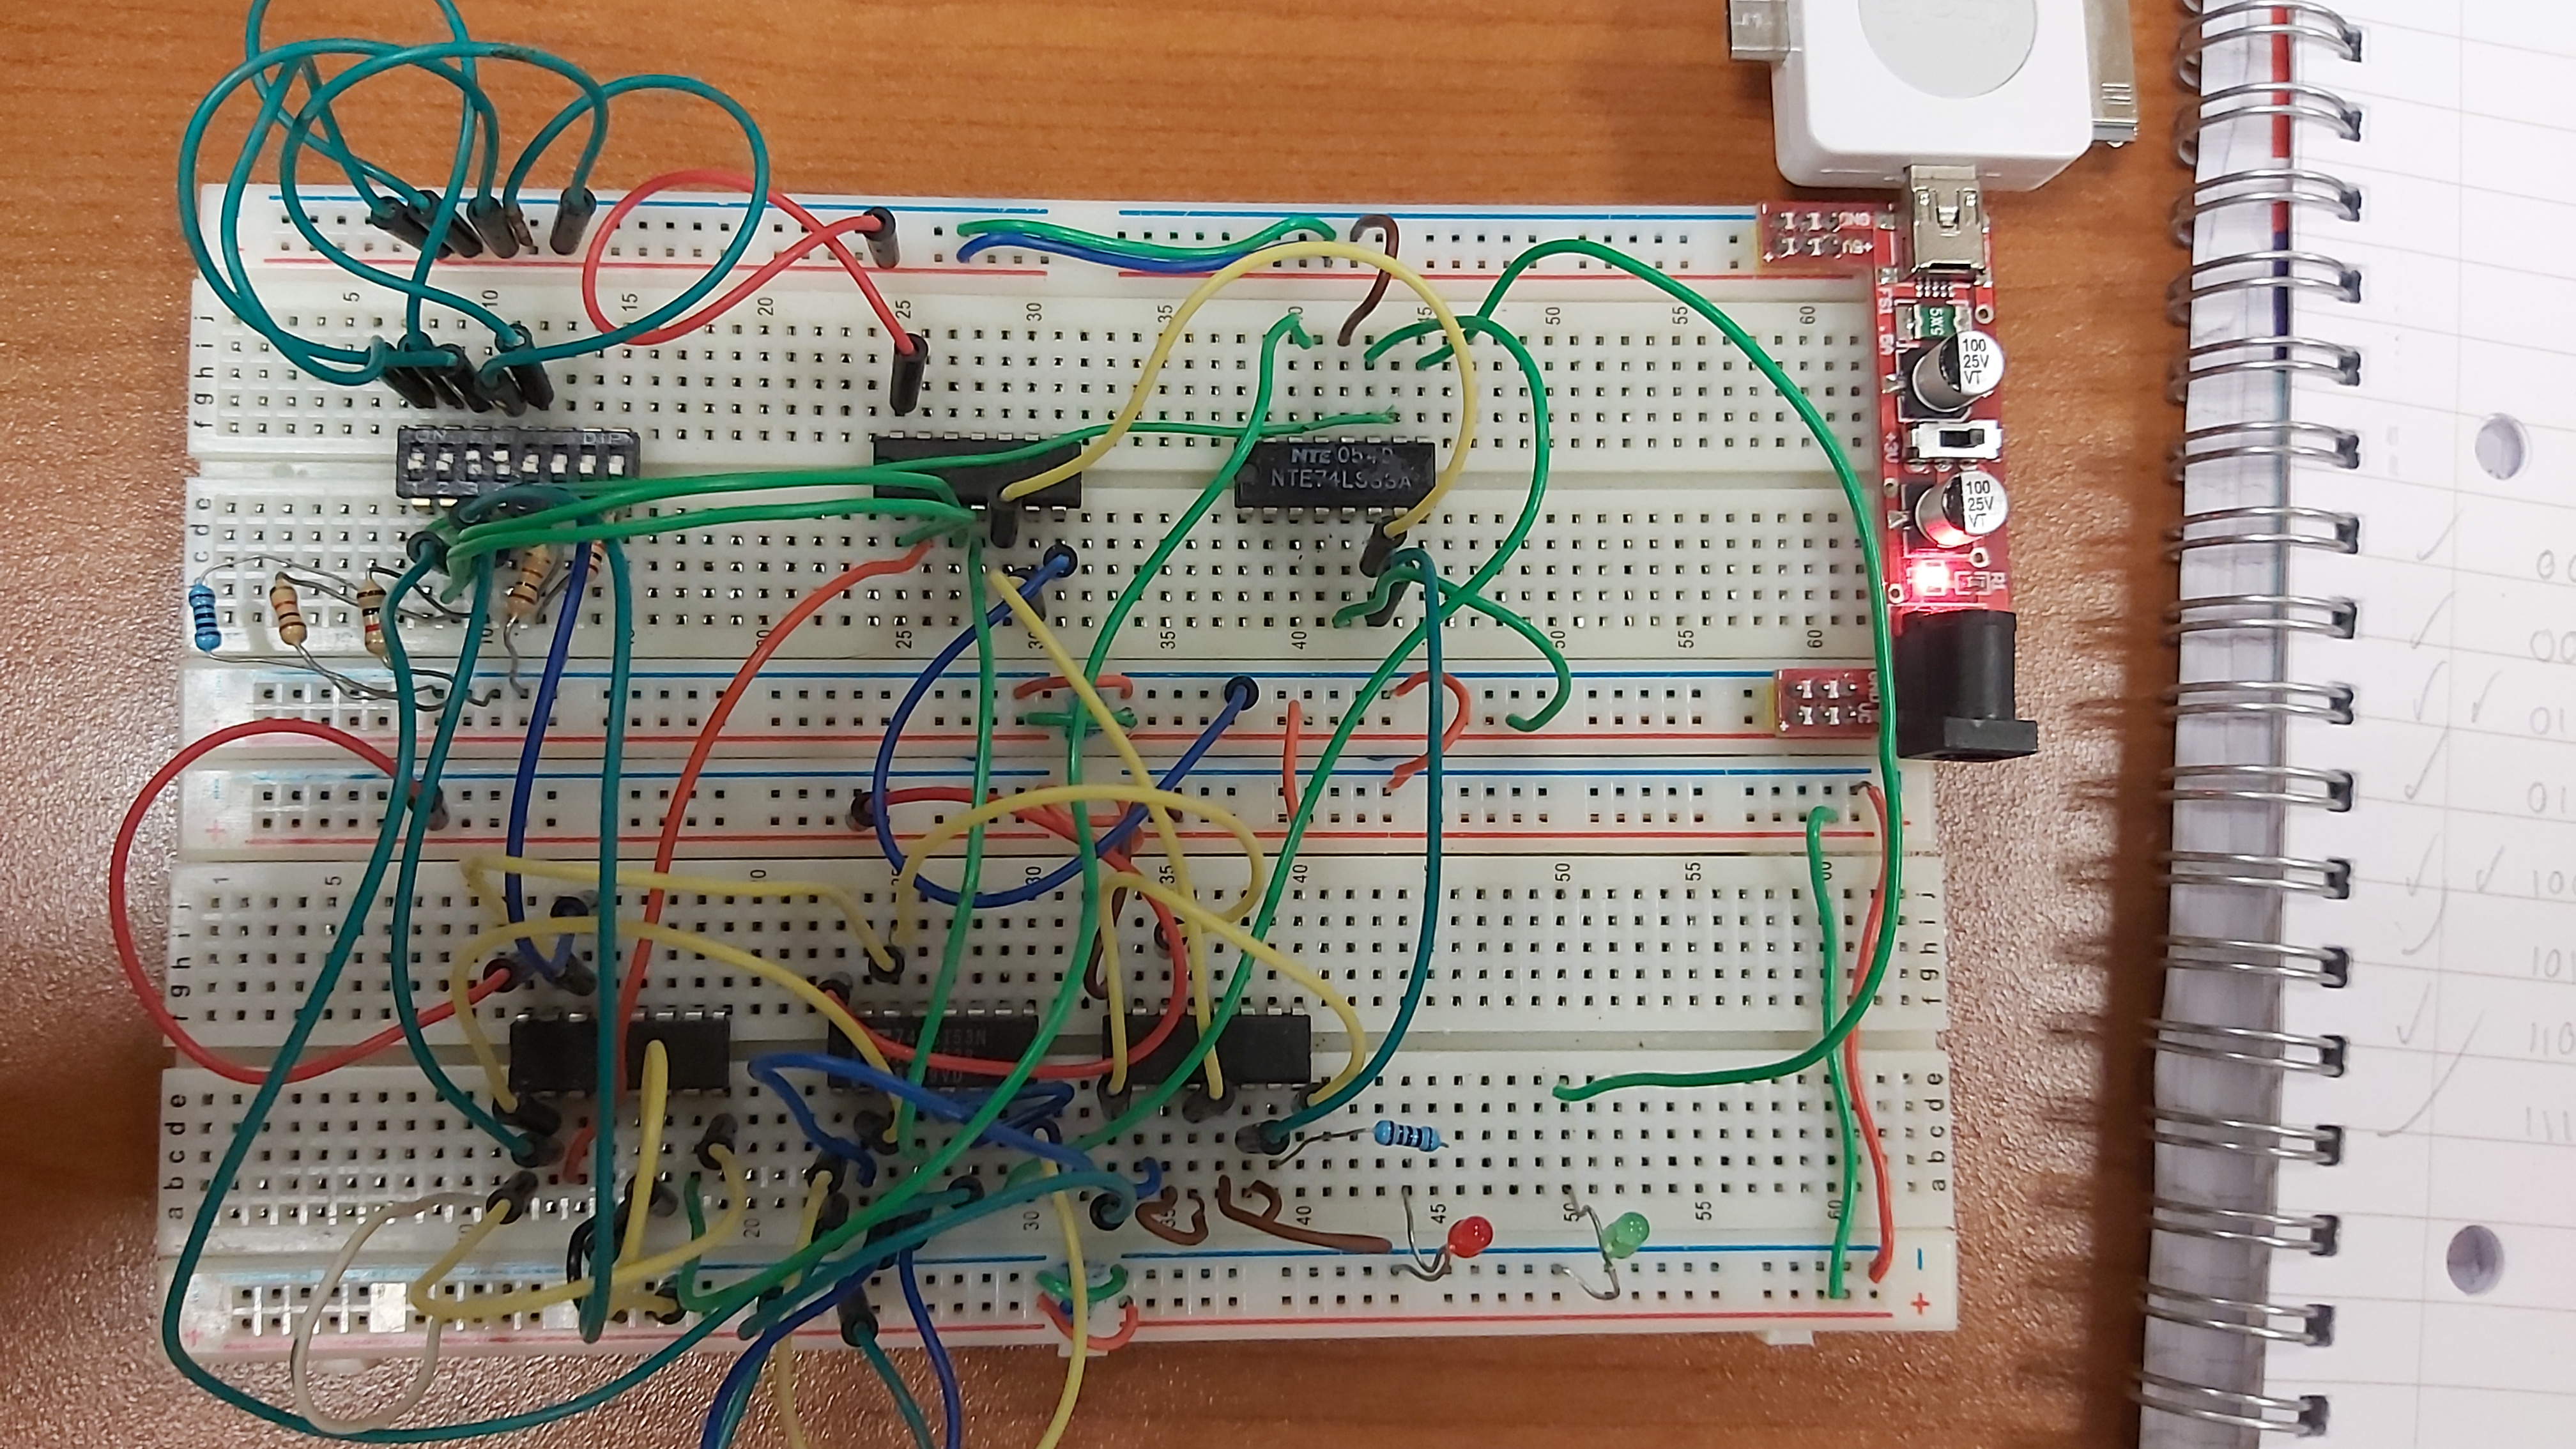
\includegraphics[width=\textwidth]{./figures/00110.jpg}
\begin{center}
	$ABC_i = 001$ and so $C_o Y= 00$.\\
\end{center}


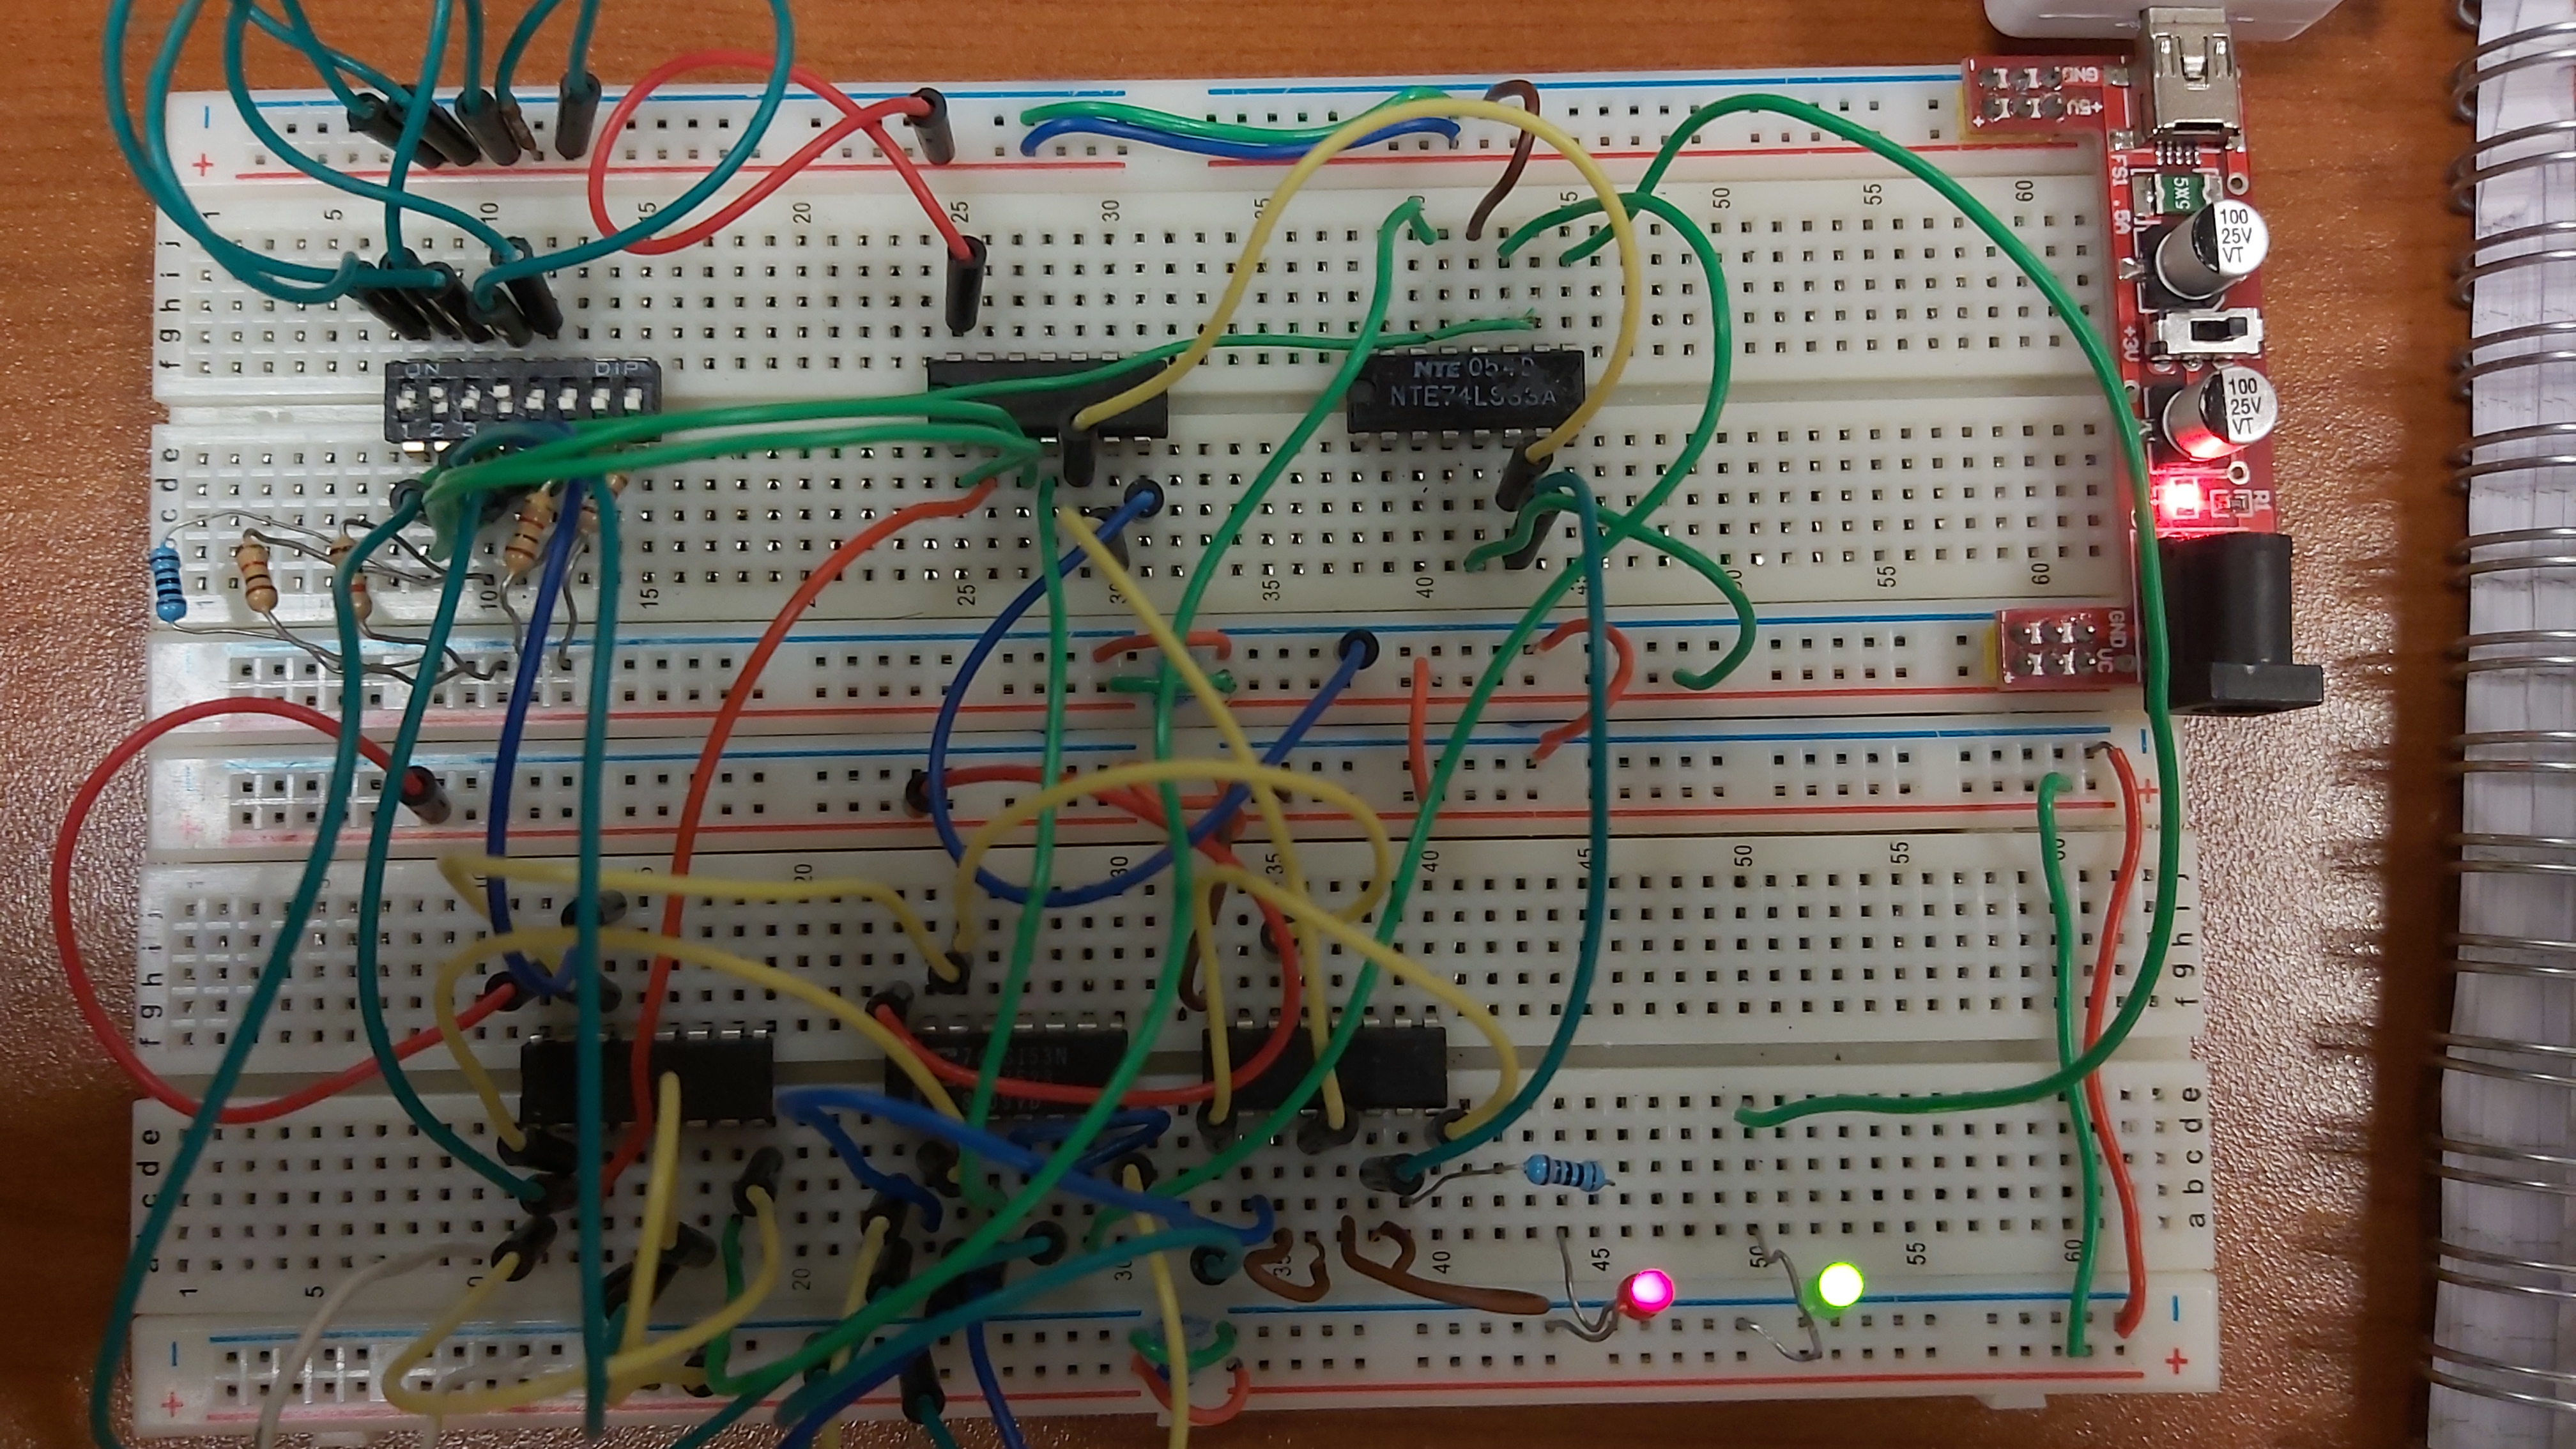
\includegraphics[width=\textwidth]{./figures/01010.jpg}
\begin{center}
	$ABC_i = 010$ and so $C_o Y= 11$.
\end{center}

\vspace{2em}

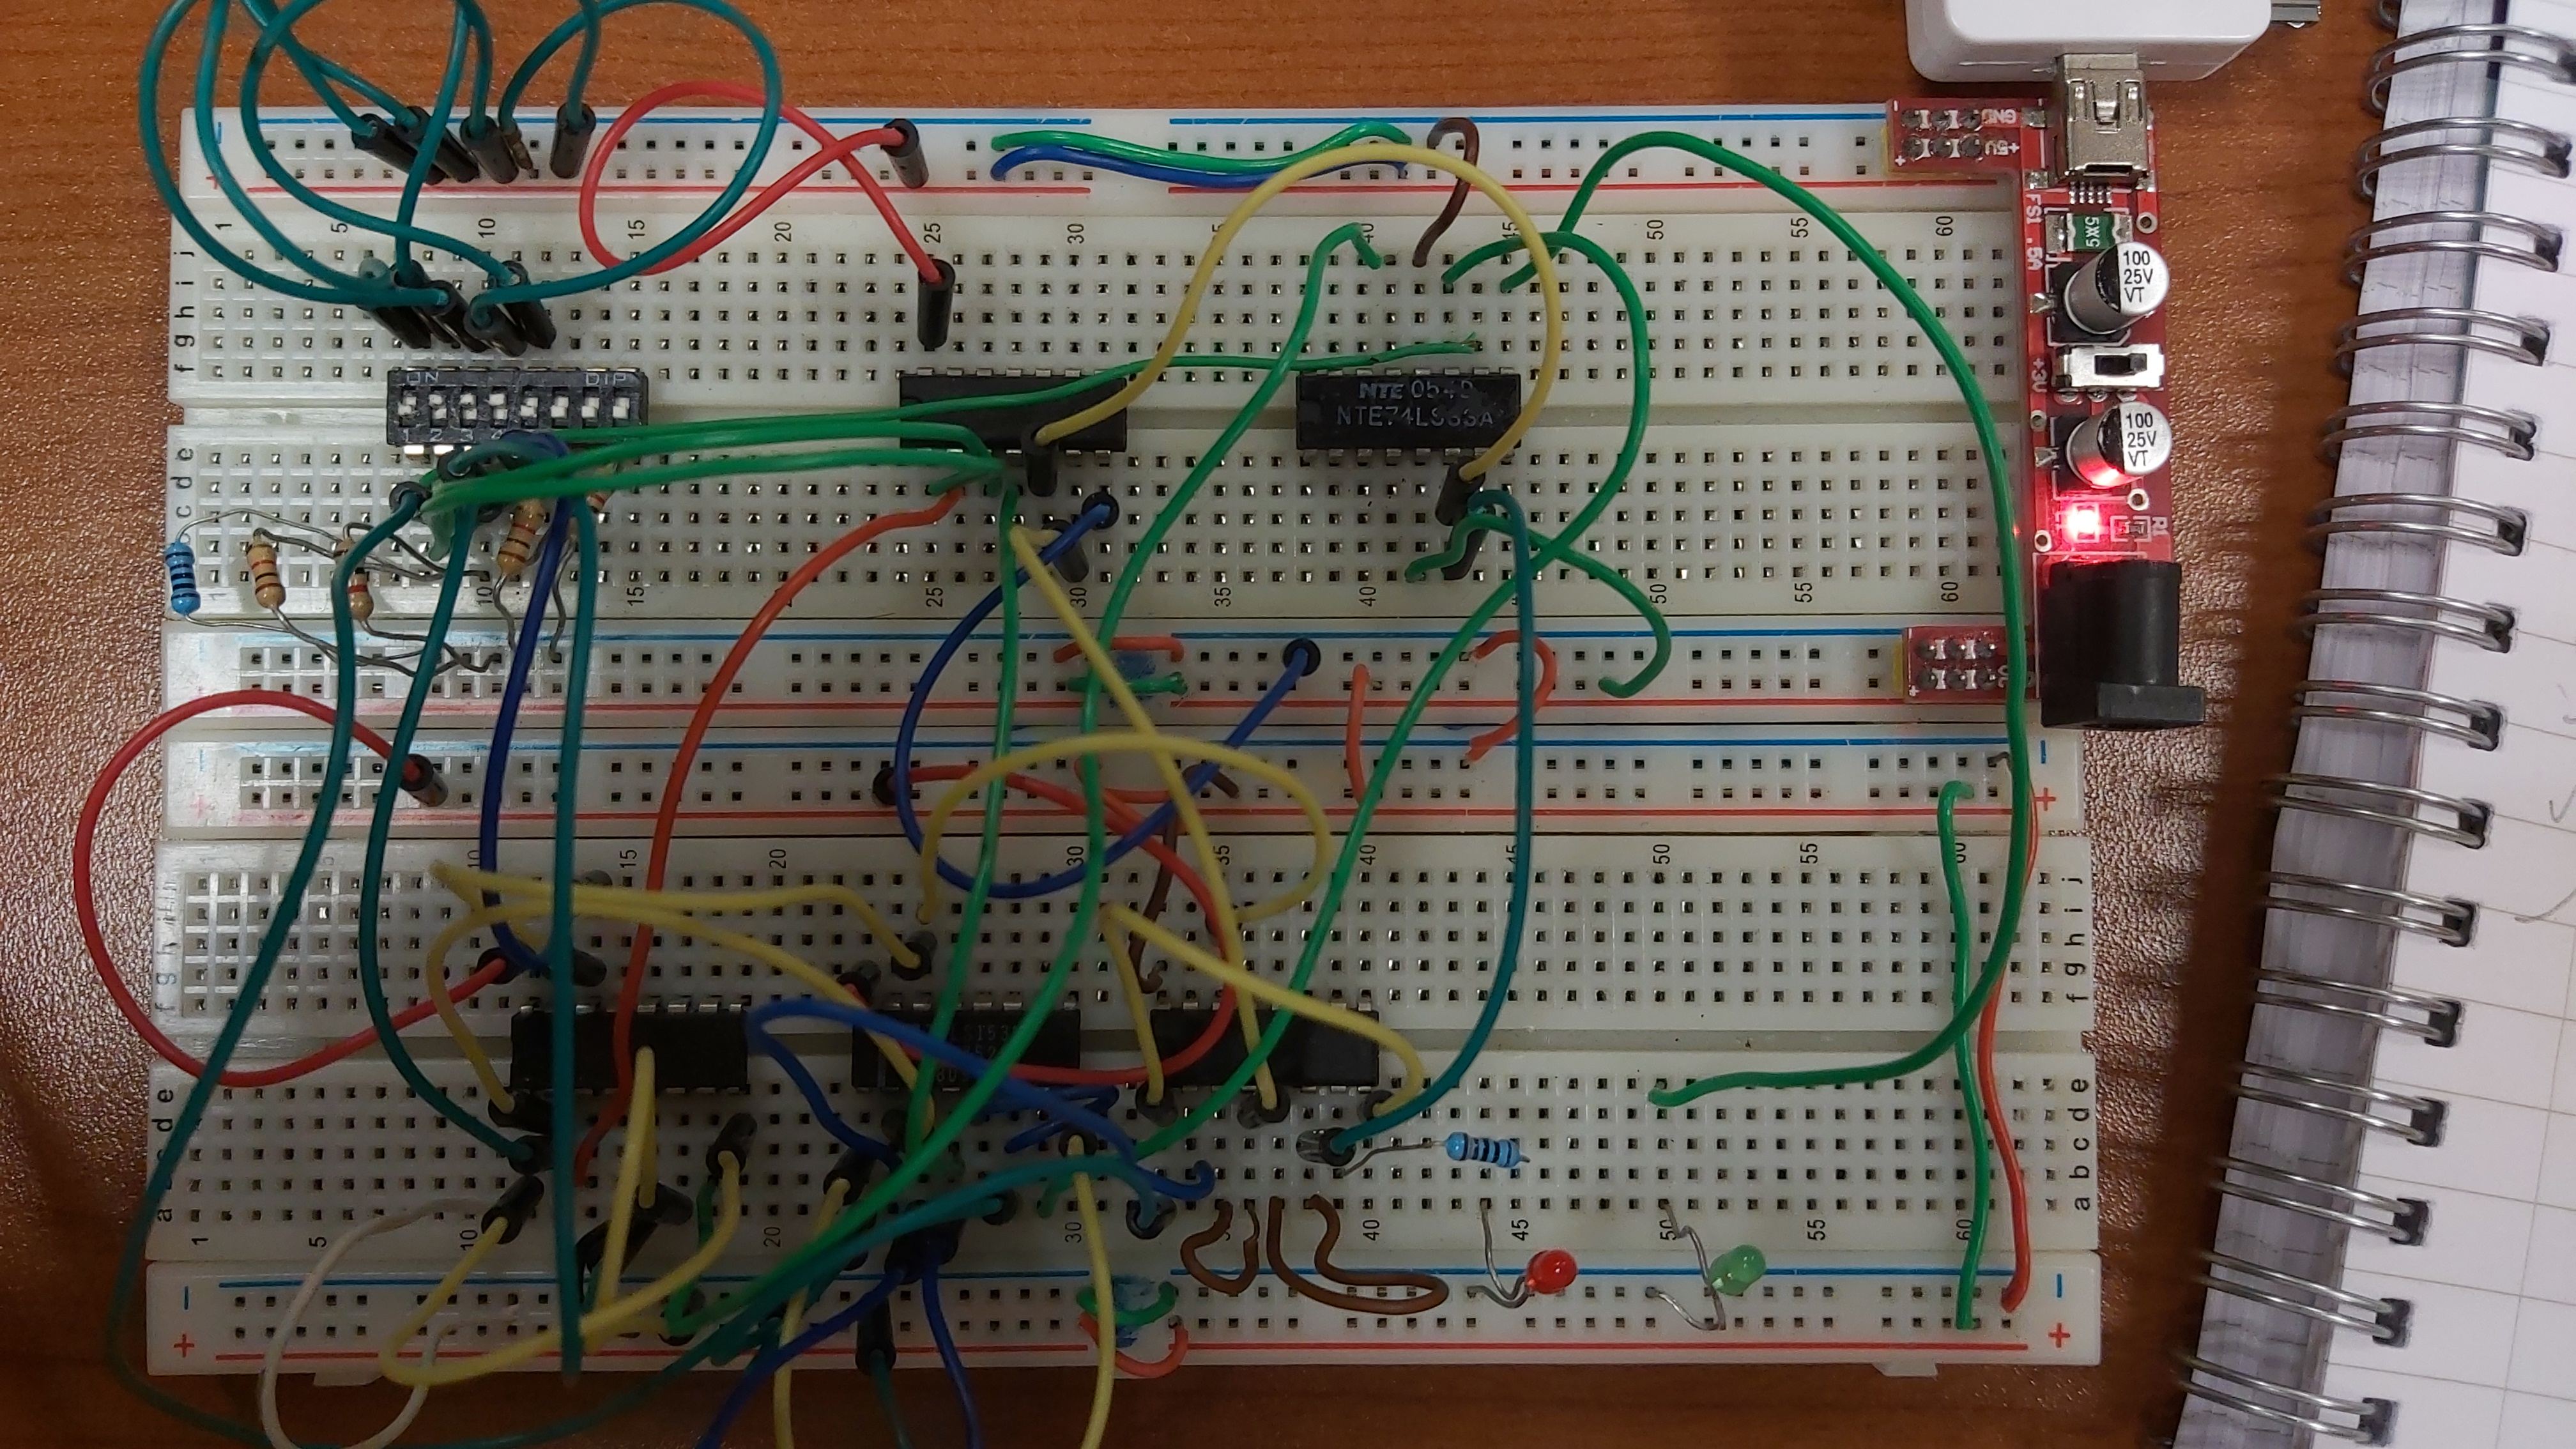
\includegraphics[width=\textwidth]{./figures/01110.jpg}
\begin{center}
	$ABC_i = 011$ and so $C_o Y= 00$.
\end{center}


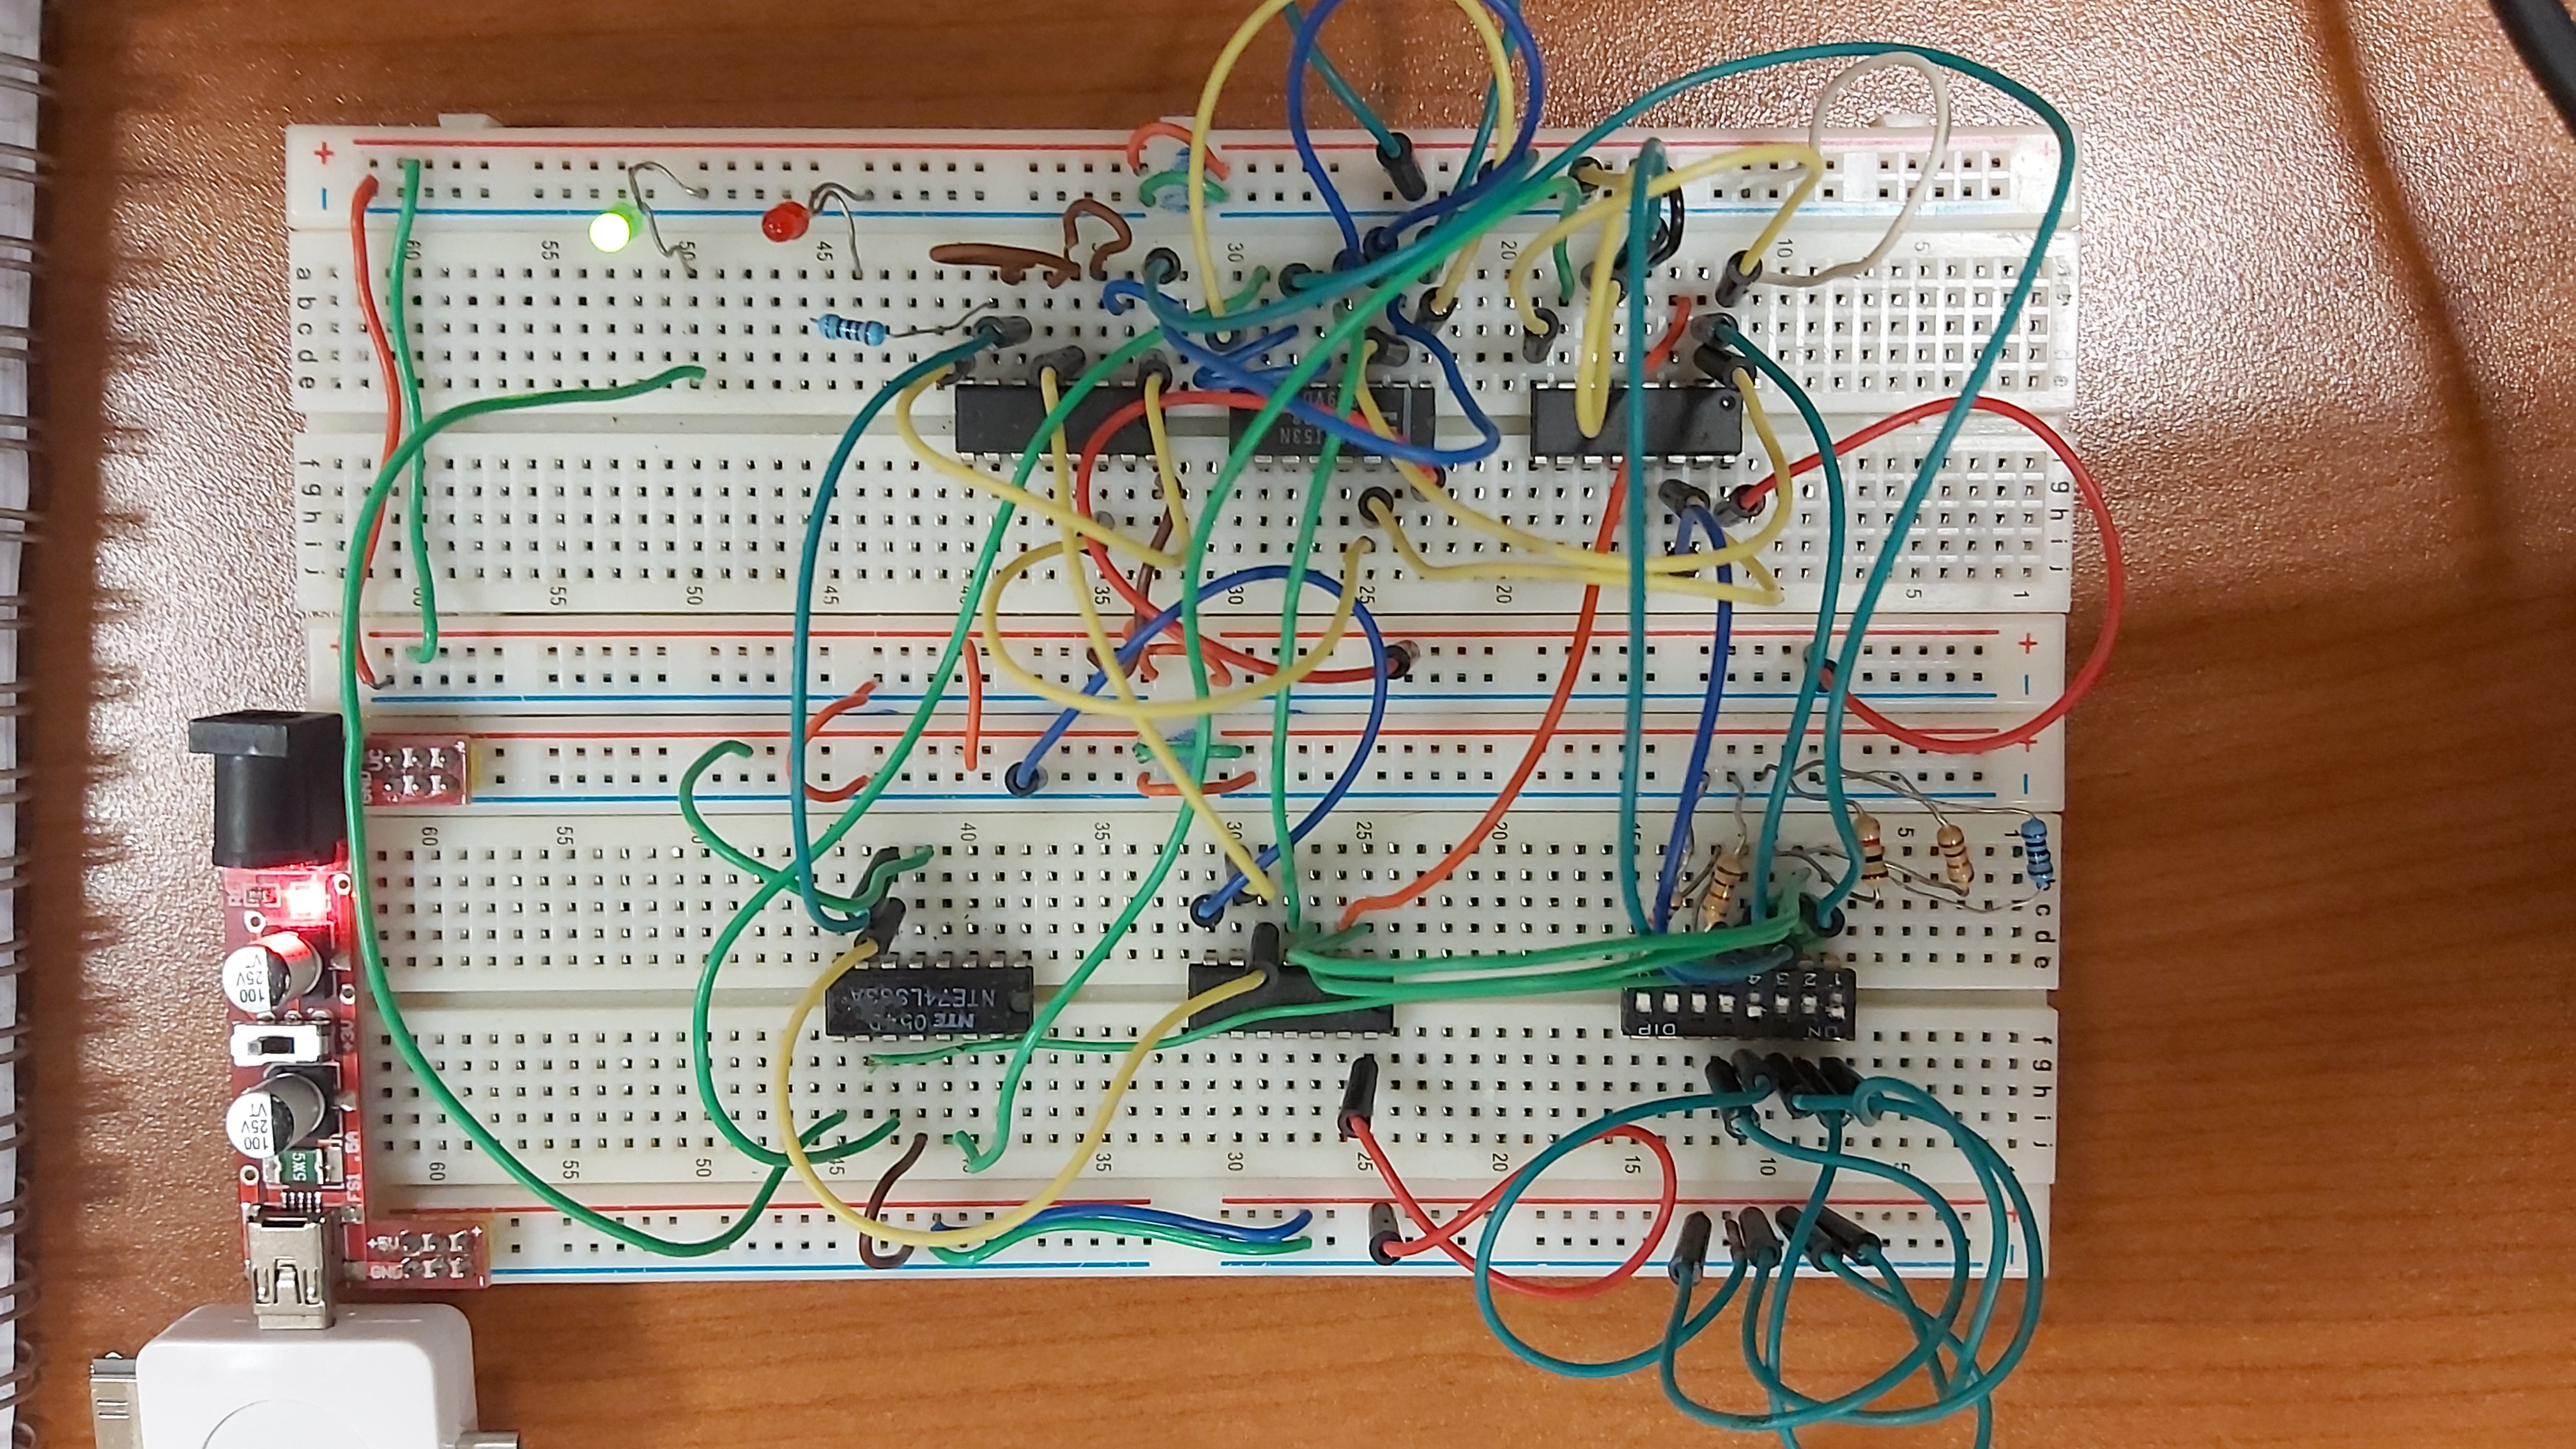
\includegraphics[angle=180, width=\textwidth]{./figures/10010.jpg}
\begin{center}
	$ABC_i = 100$ and so $C_o Y= 01$.
\end{center}

\vspace{2em}

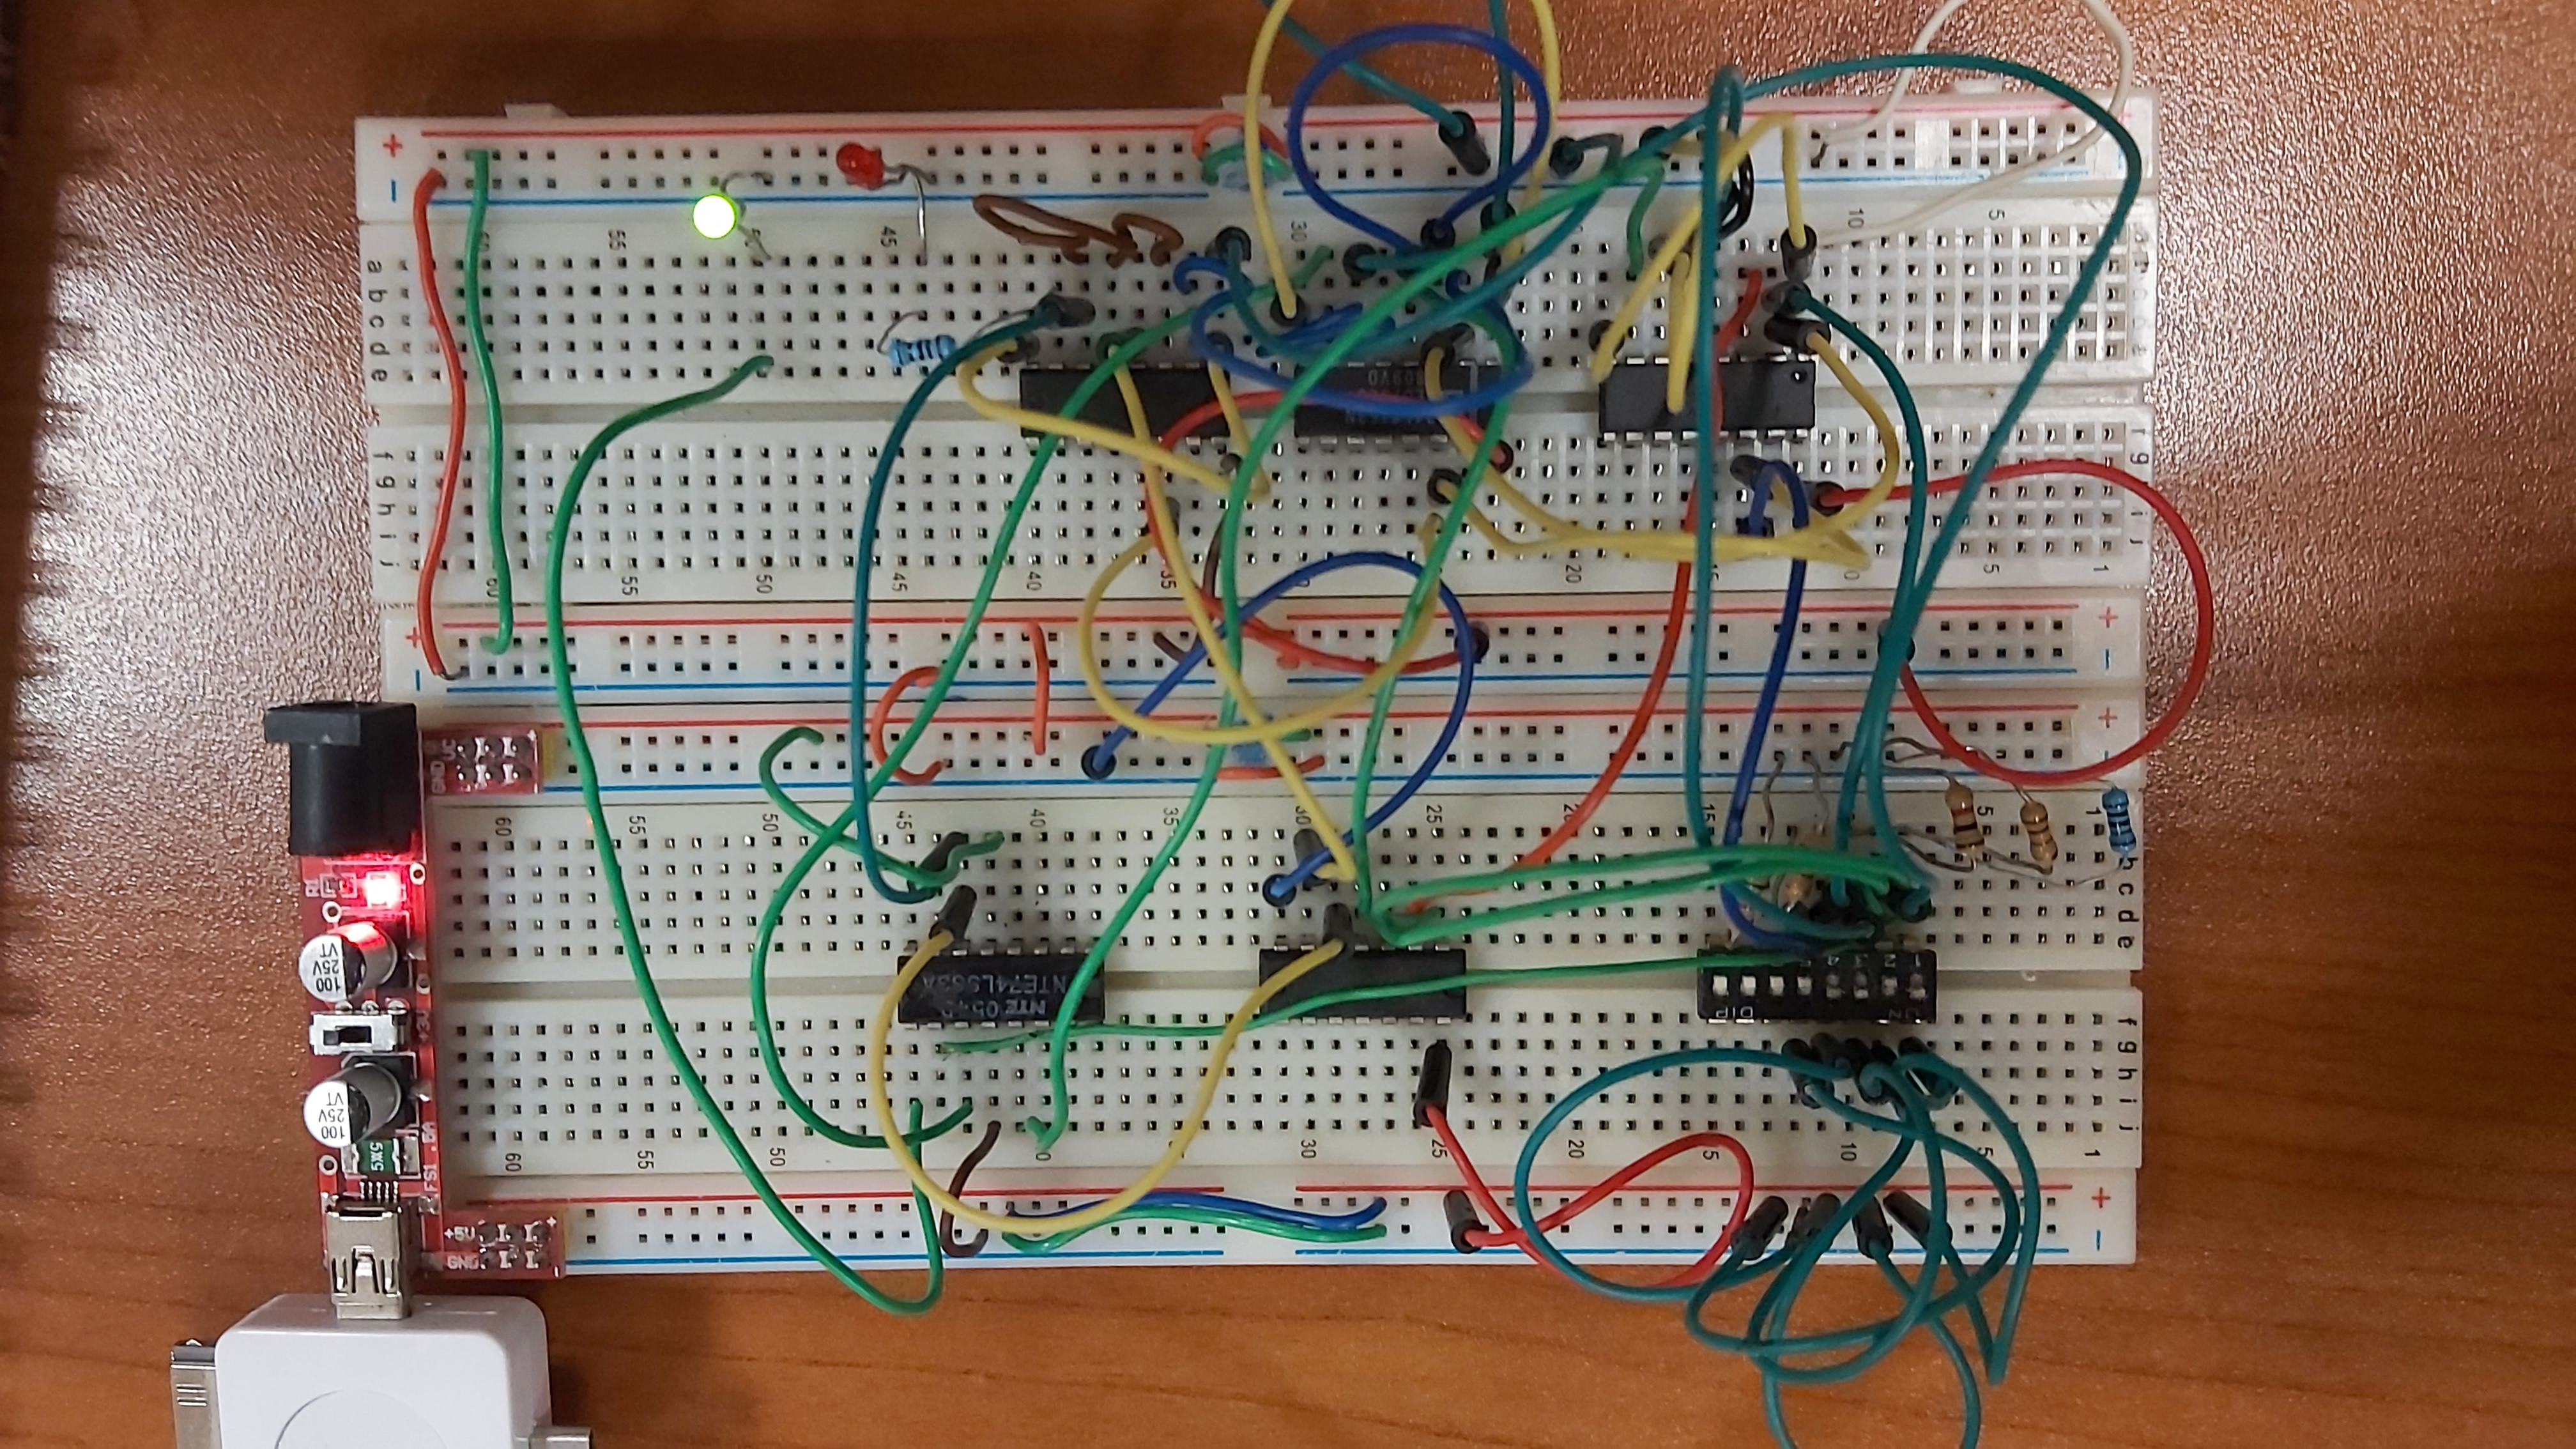
\includegraphics[angle=180, width=\textwidth]{./figures/10110.jpg}
\begin{center}
	$ABC_i = 101$ and so $C_o Y= 01$.
\end{center}


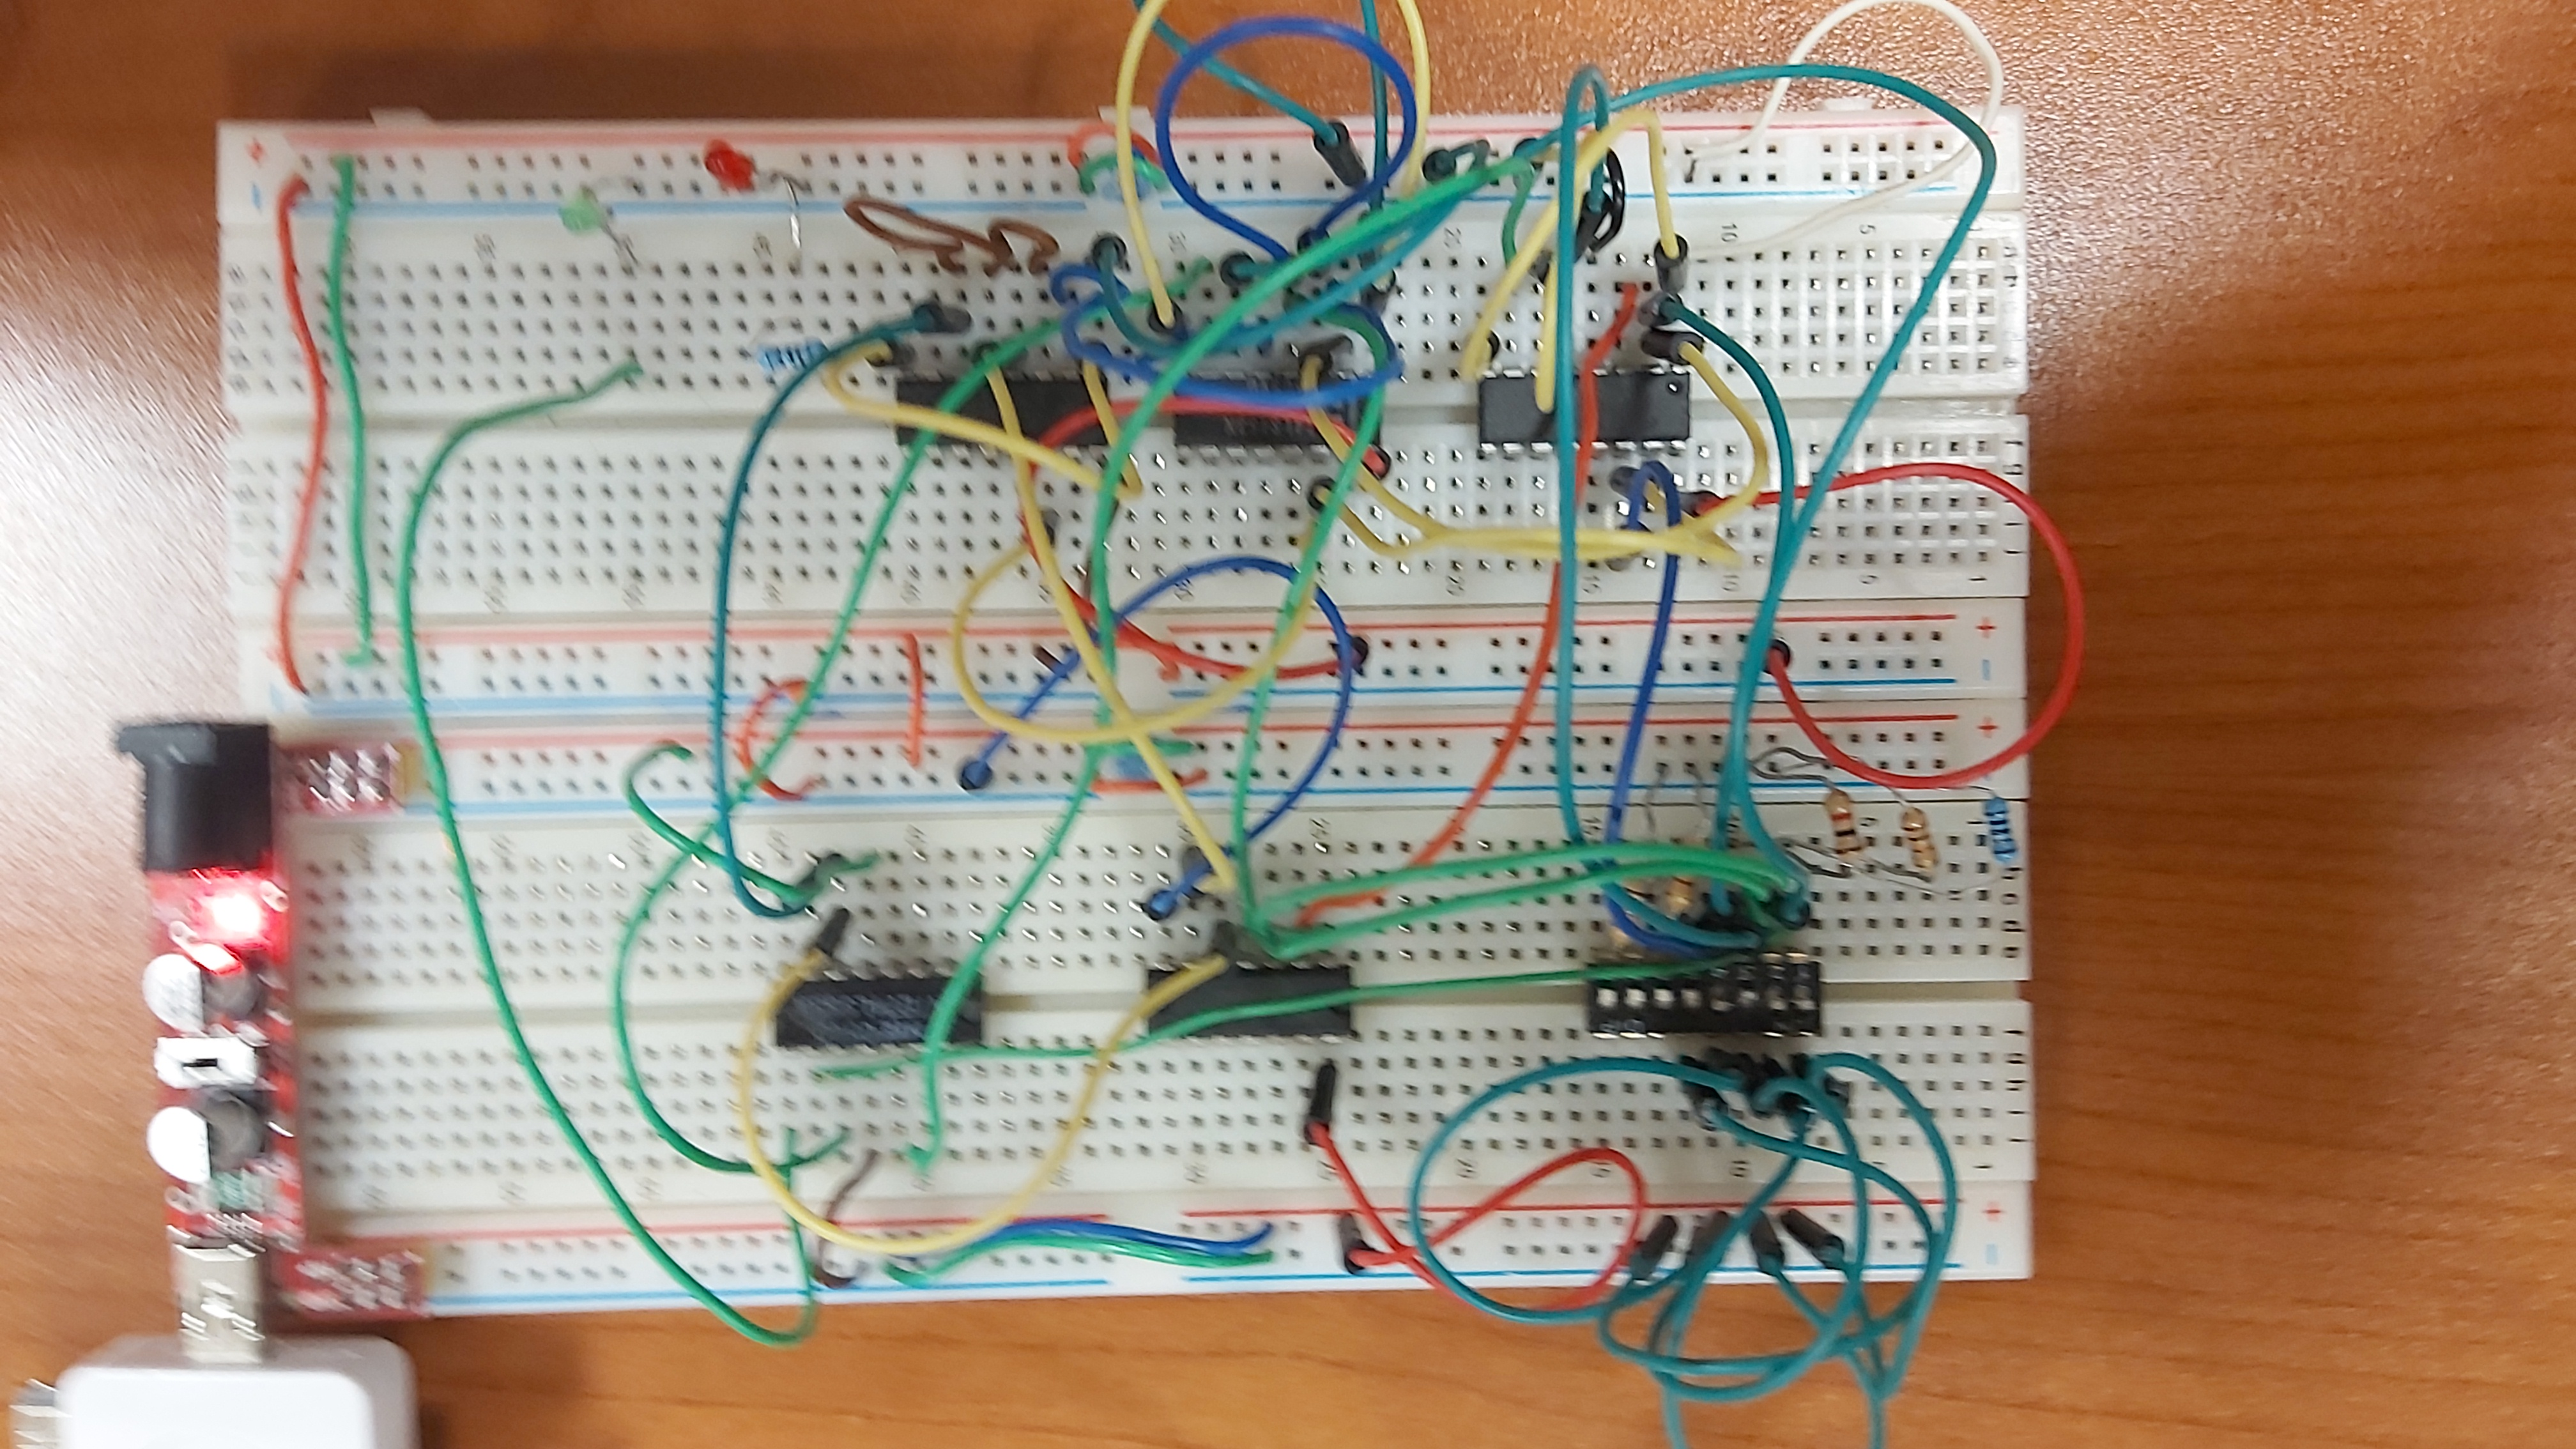
\includegraphics[angle=180, width=\textwidth]{./figures/11010.jpg}
\begin{center}
	$ABC_i = 110$ and so $C_o Y= 00$.
\end{center}

\vspace{2em}

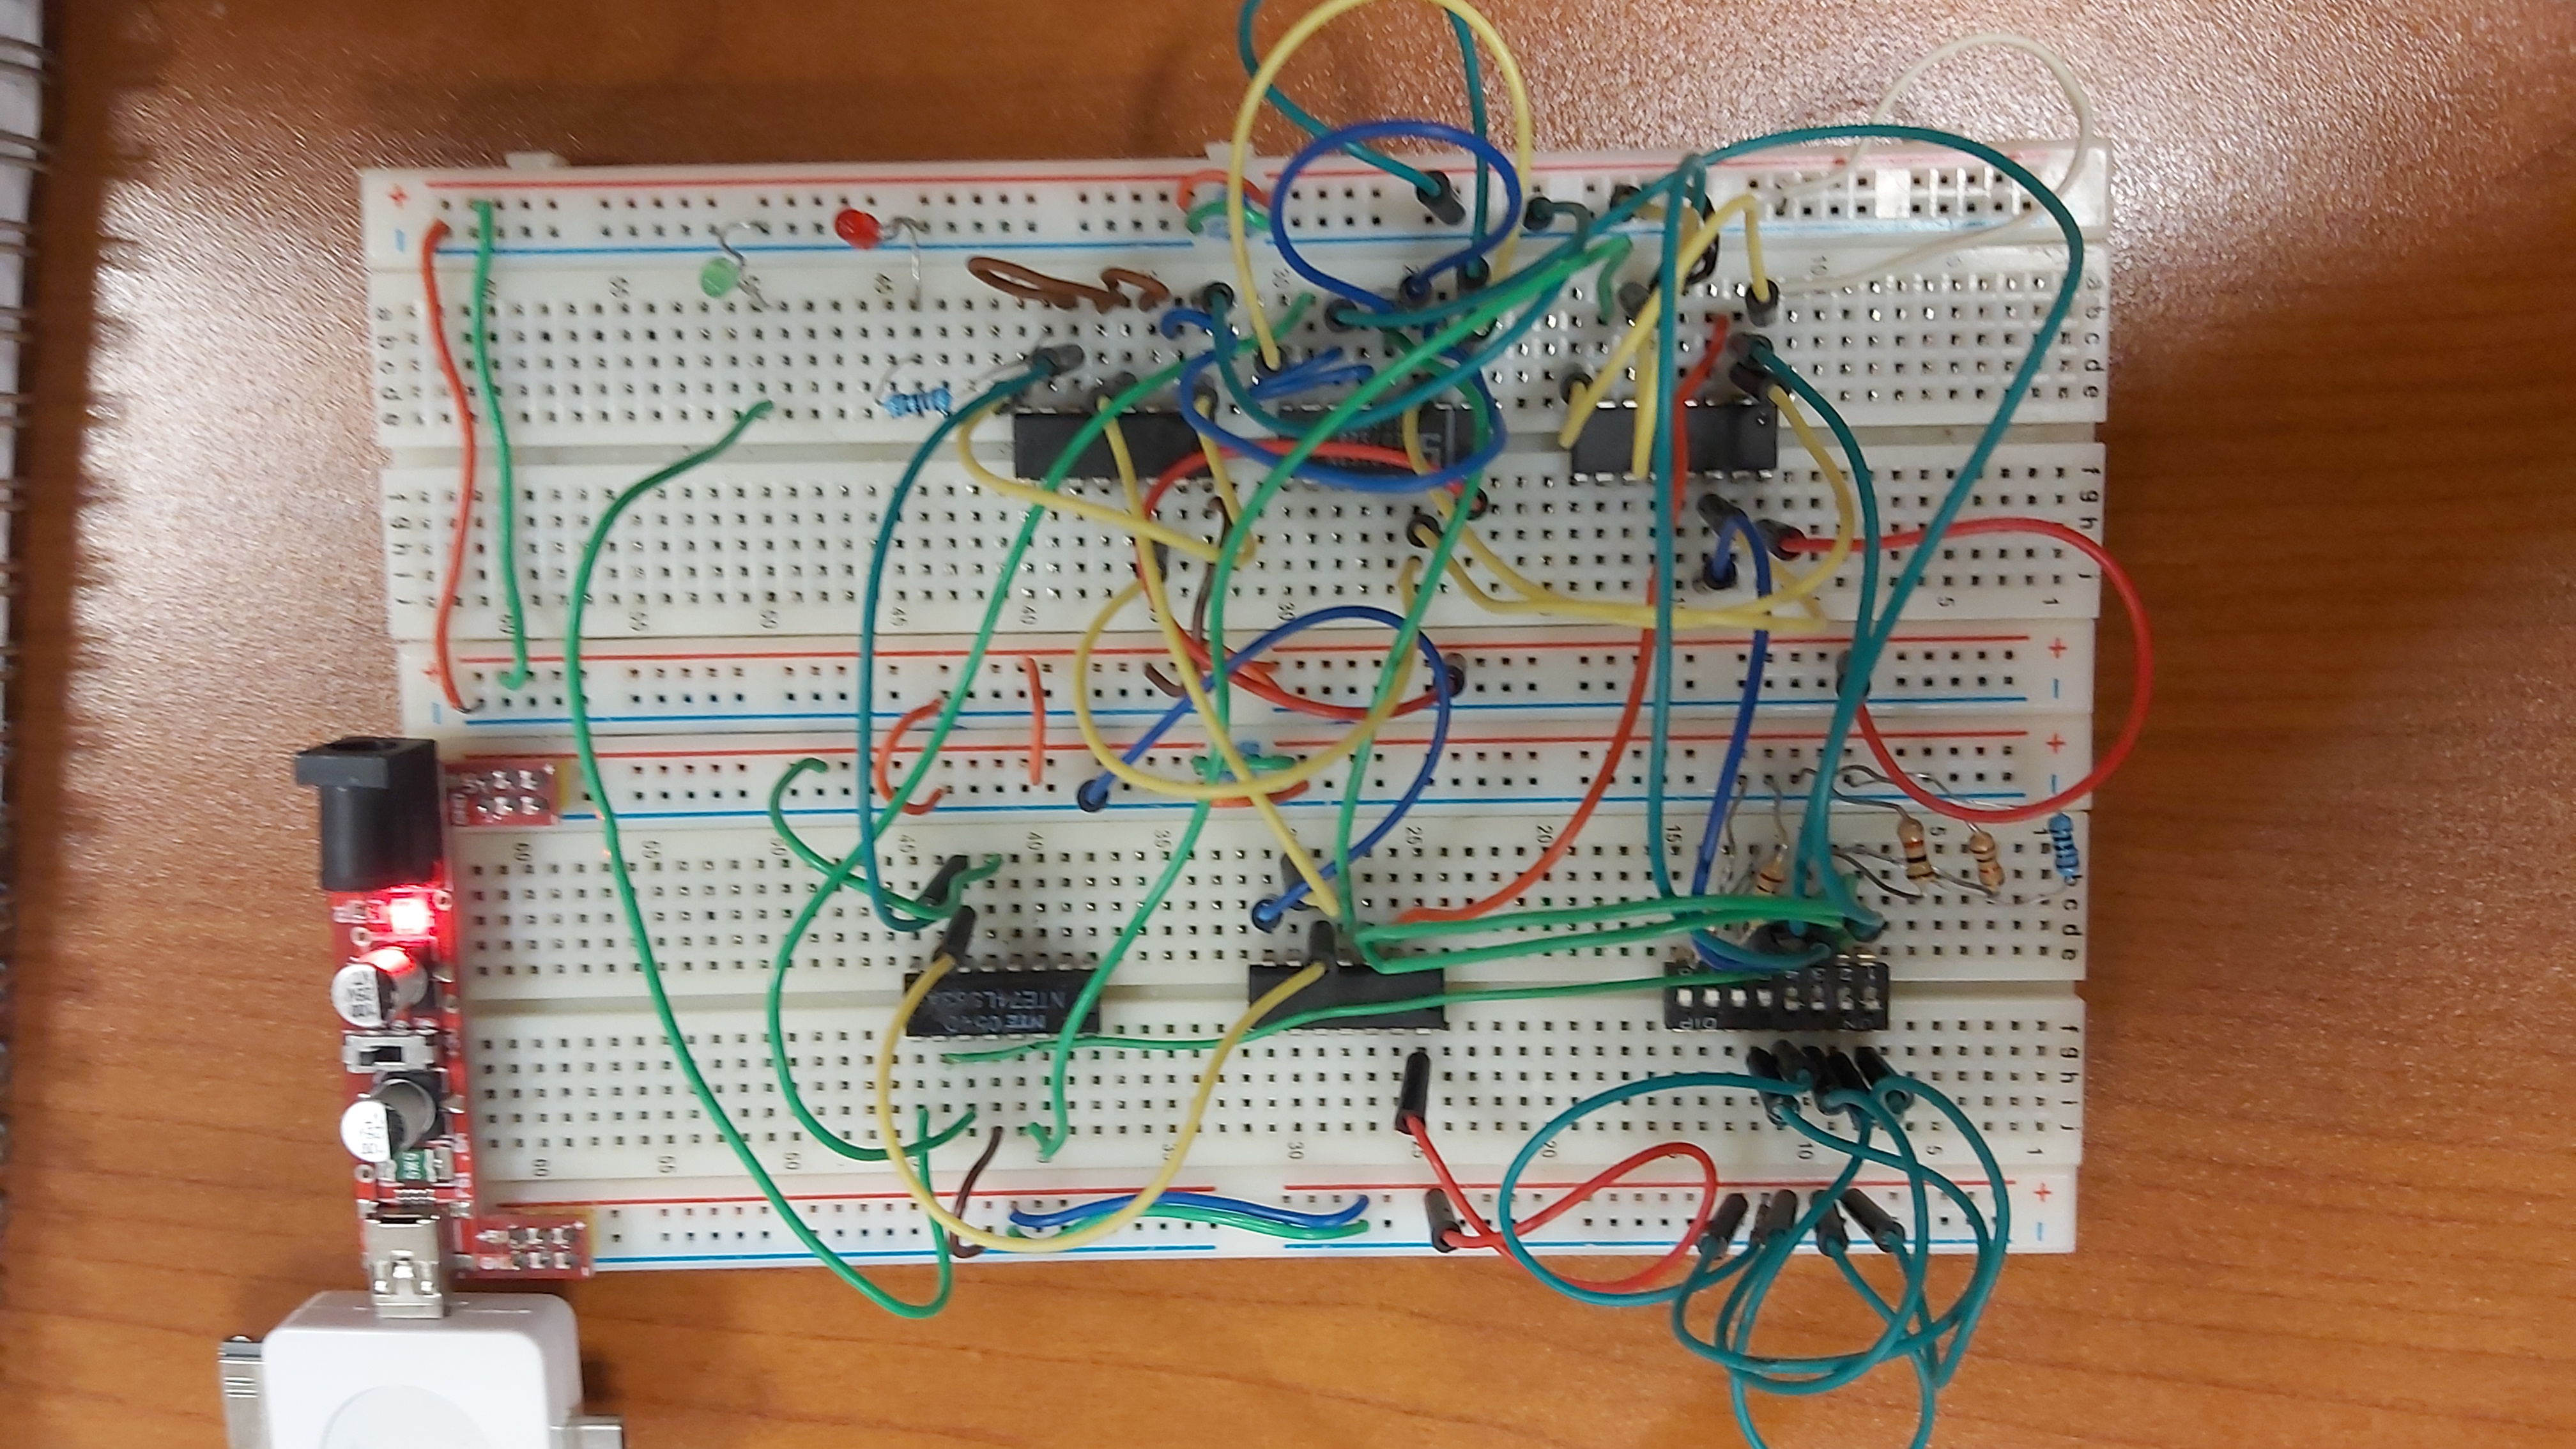
\includegraphics[angle=180, width=\textwidth]{./figures/11110.jpg}
\begin{center}
	$ABC_i = 111$ and so $C_o Y= 00$.
\end{center}


\subsection{Opcode \texttt{11 - SUBB}}

With this opcode selected, the ALU performs the subtraction of bits $A$ and $B$, or rather, the
addition of $A$ and $\bar{B}$, whilst ignoring the borrow bit $C_{i}$. When a negative value is
obtained, the resultant representation will be one in 2's complement, and so $-1_{10}$ would be
represented as $11_2 = -2_{10} + 1_{10}$.

\[A+\bar{B}+\bar{C_i} = C_o Y\]

\vspace{9em}

\subsubsection{Truth table}

\begin{center}
	\Large
	\begin{tabular}{c|c|c||c|c||c|c|c}
		$A$ & $B$ & $C_i$ & $Op_1$ & $Op_2$ & $C_{o}$ & $Y$ \\
		\hline
		0 & 0 & 0 & 1 & 1 & 0 & 0 \\
		0 & 0 & 1 & 1 & 1 & 1 & 1 \\%
		0 & 1 & 0 & 1 & 1 & 1 & 1 \\%
		0 & 1 & 1 & 1 & 1 & 1 & 0 \\%
		1 & 0 & 0 & 1 & 1 & 0 & 1 \\
		1 & 0 & 1 & 1 & 1 & 0 & 0 \\
		1 & 1 & 0 & 1 & 1 & 0 & 0 \\
		1 & 1 & 1 & 1 & 1 & 1 & 1 \\ %
	\end{tabular}
\end{center}


\newpage

\subsubsection{Pictures}

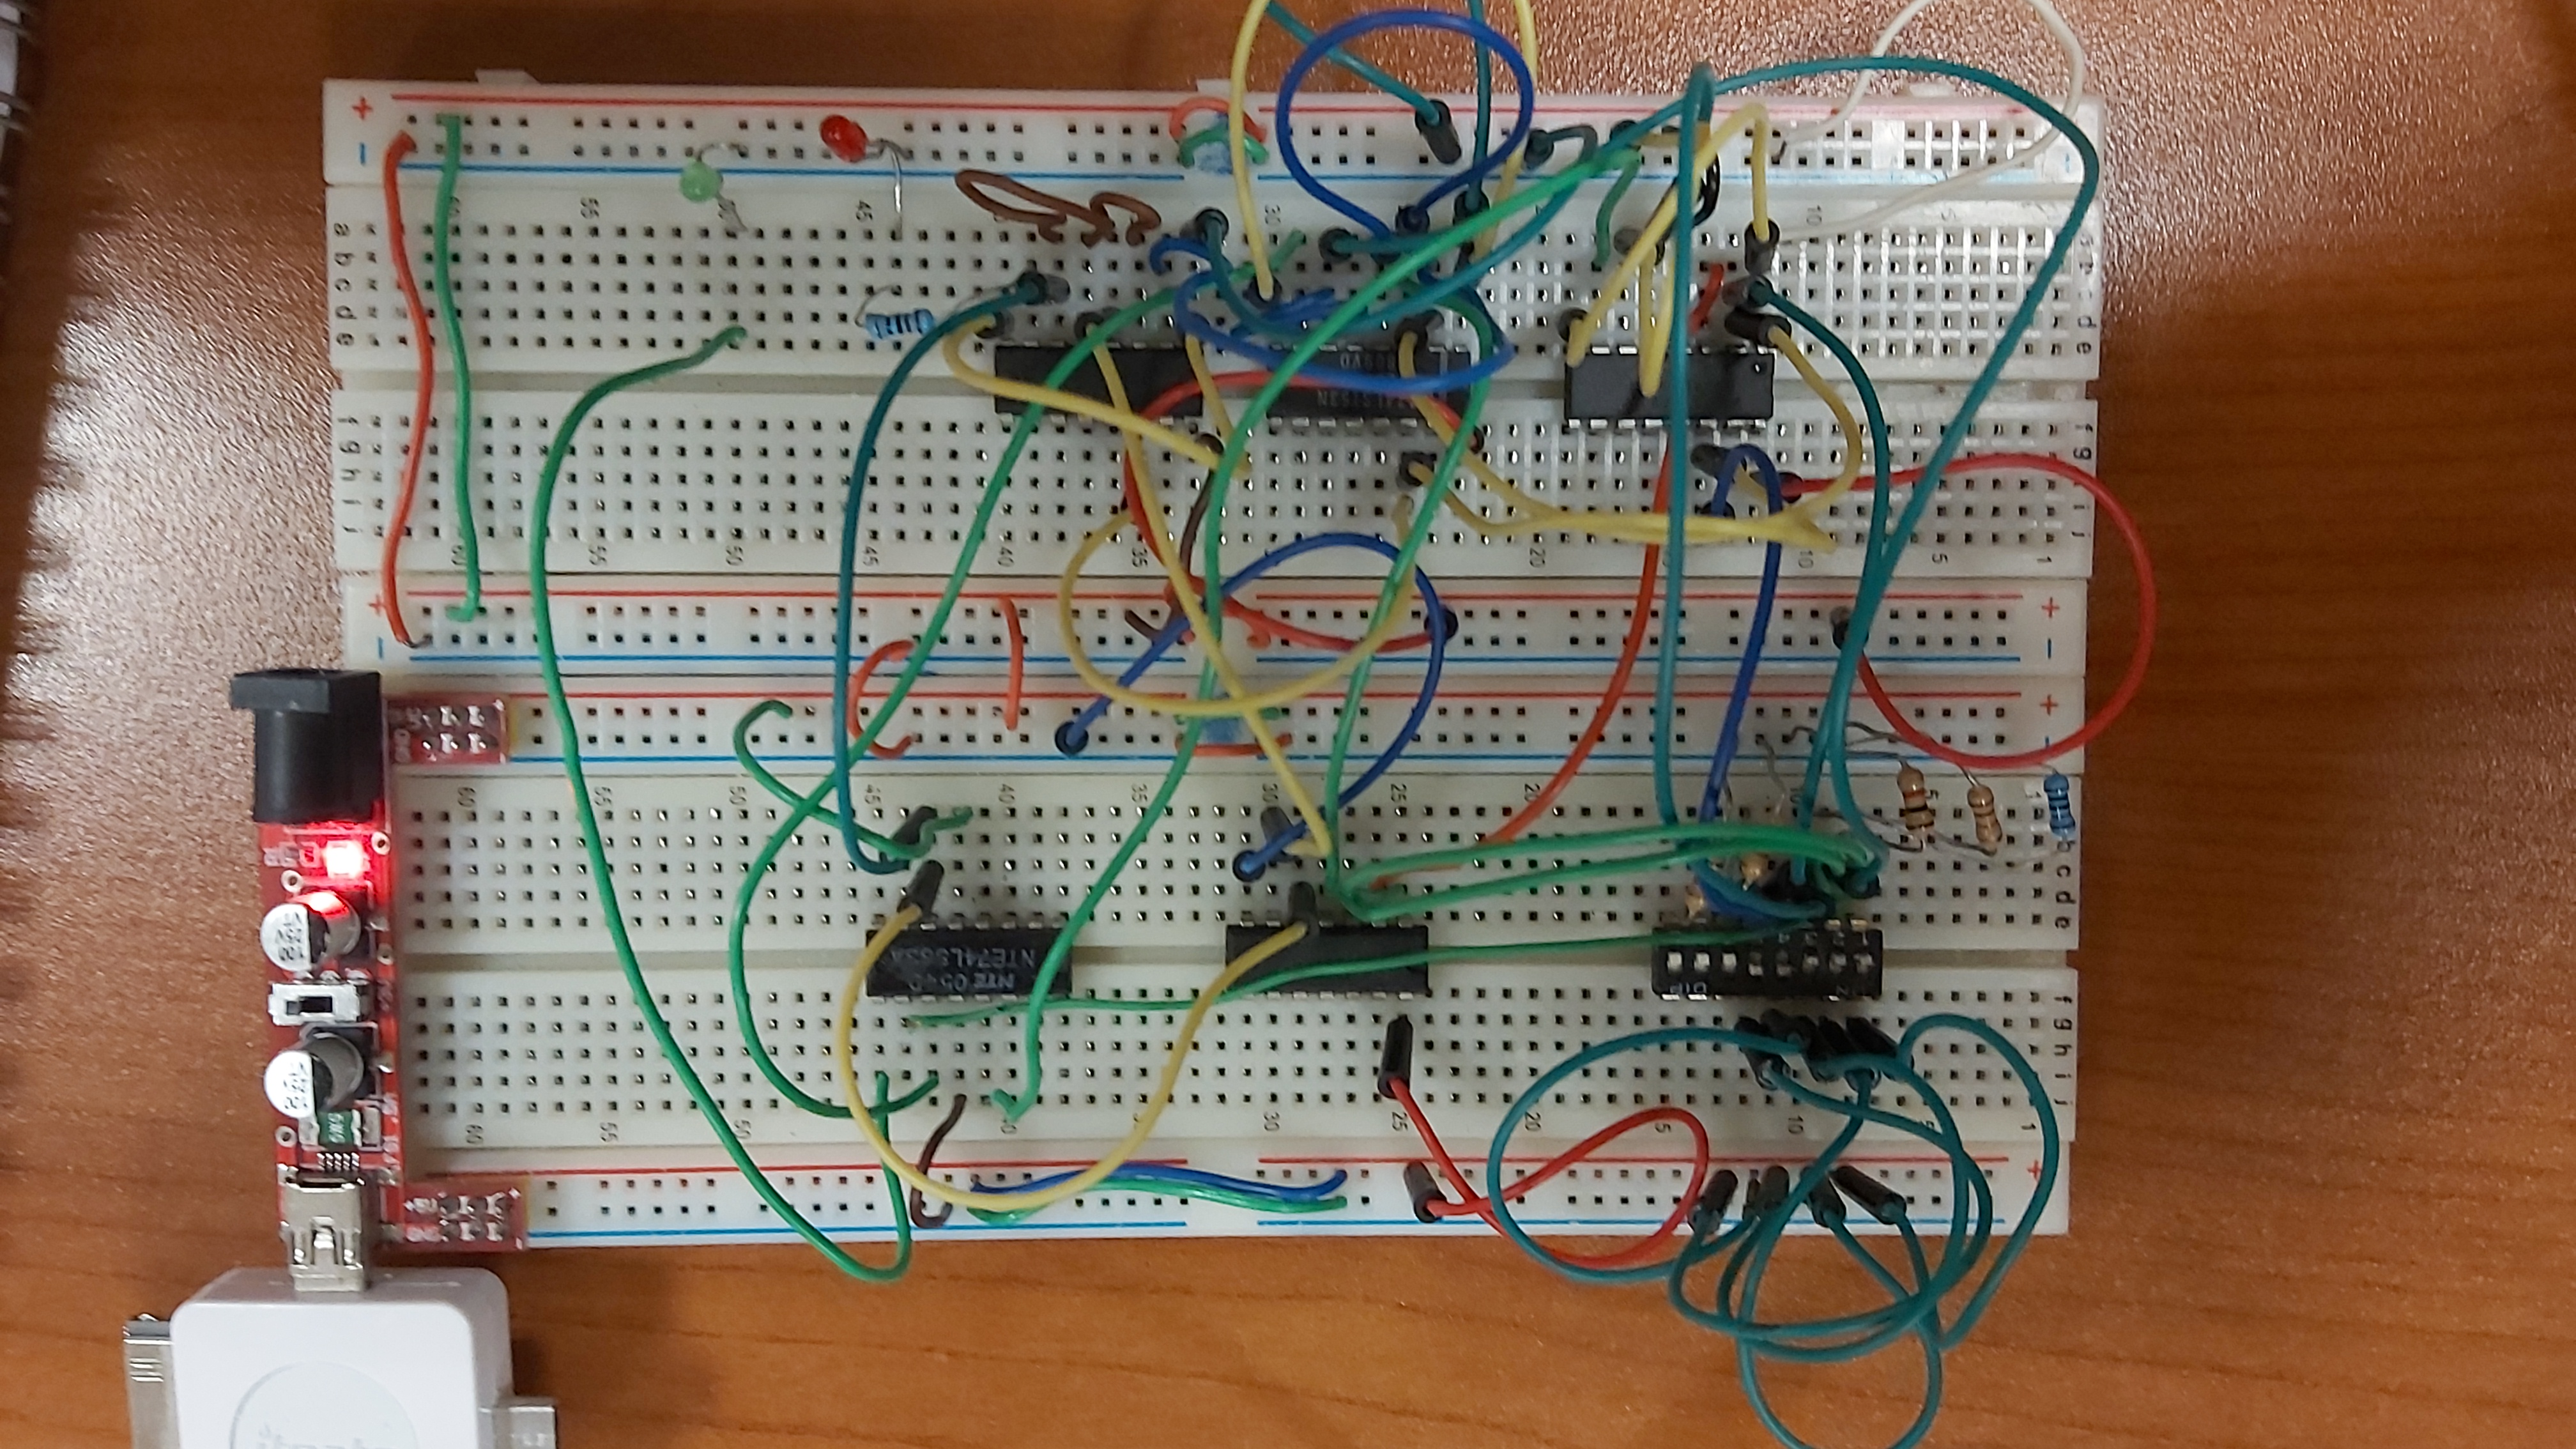
\includegraphics[angle=180, width=\textwidth]{./figures/00011.jpg}
\begin{center}
	All inputs are off, and thus no LED is on.
\end{center}

\vspace{1em}

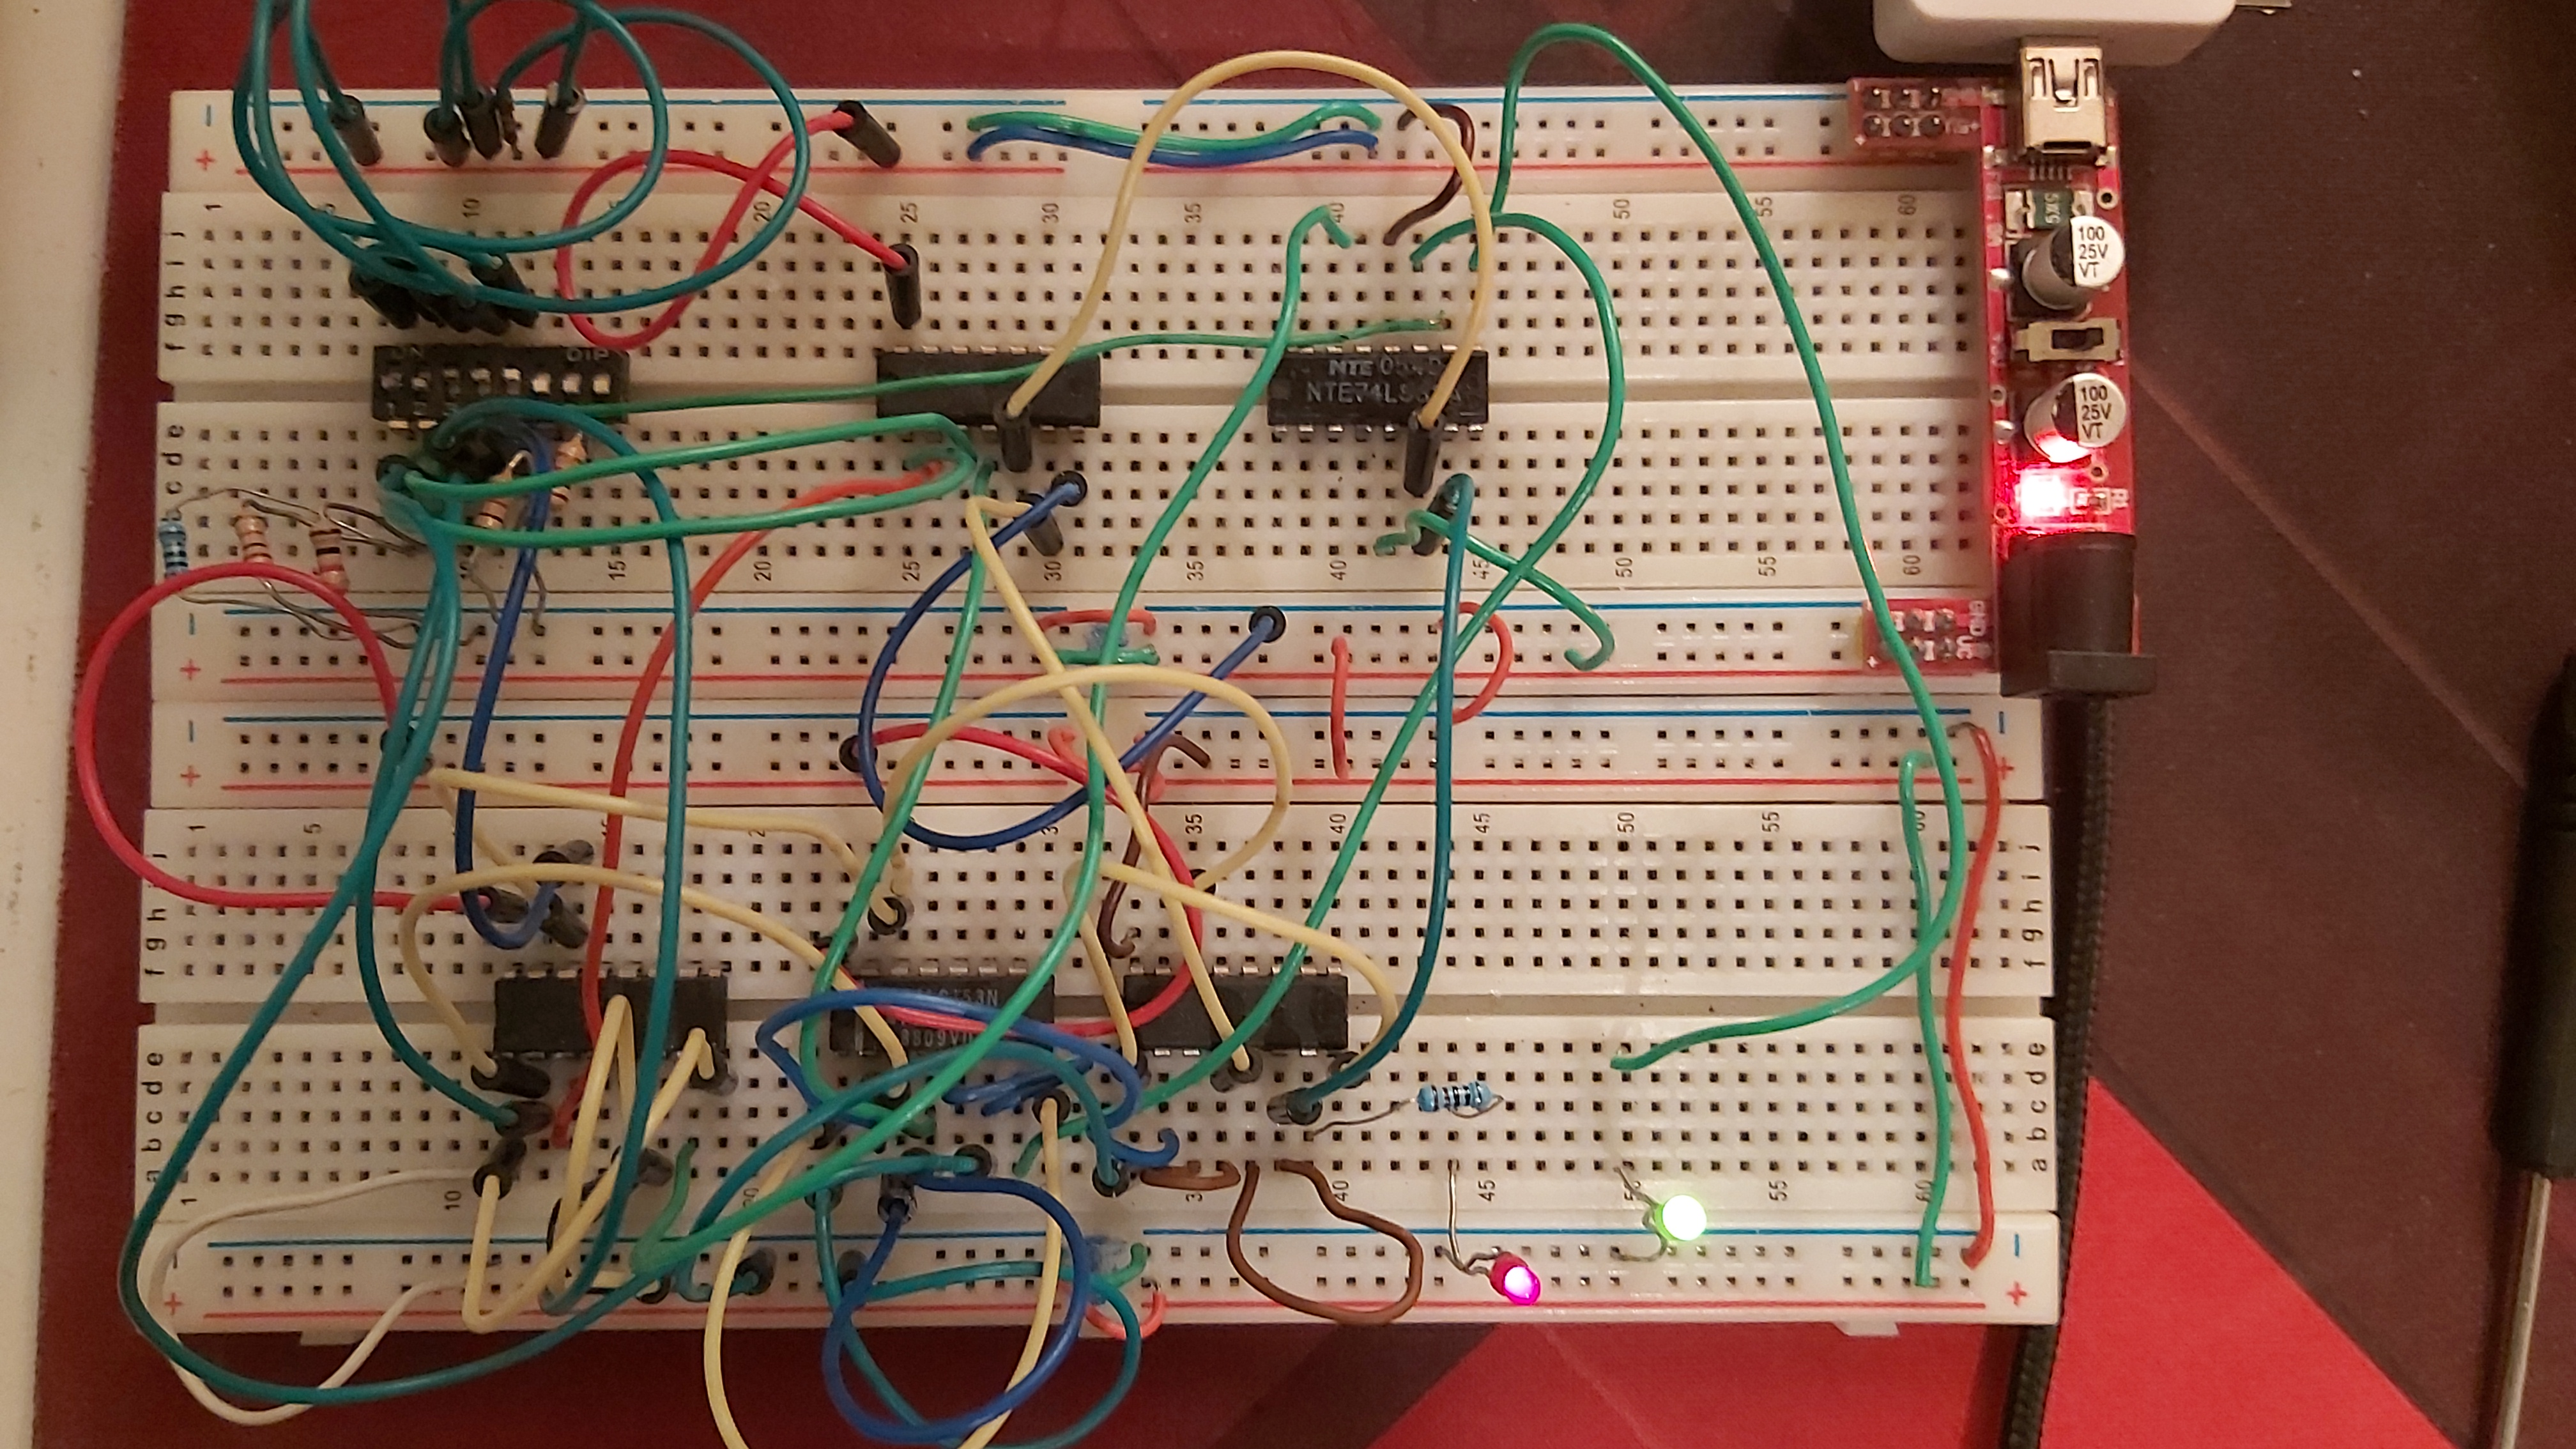
\includegraphics[width=\textwidth]{./figures/00111.jpg}
\begin{center}
	$ABC_i = 001$ and so $C_o Y= 11$.
\end{center}

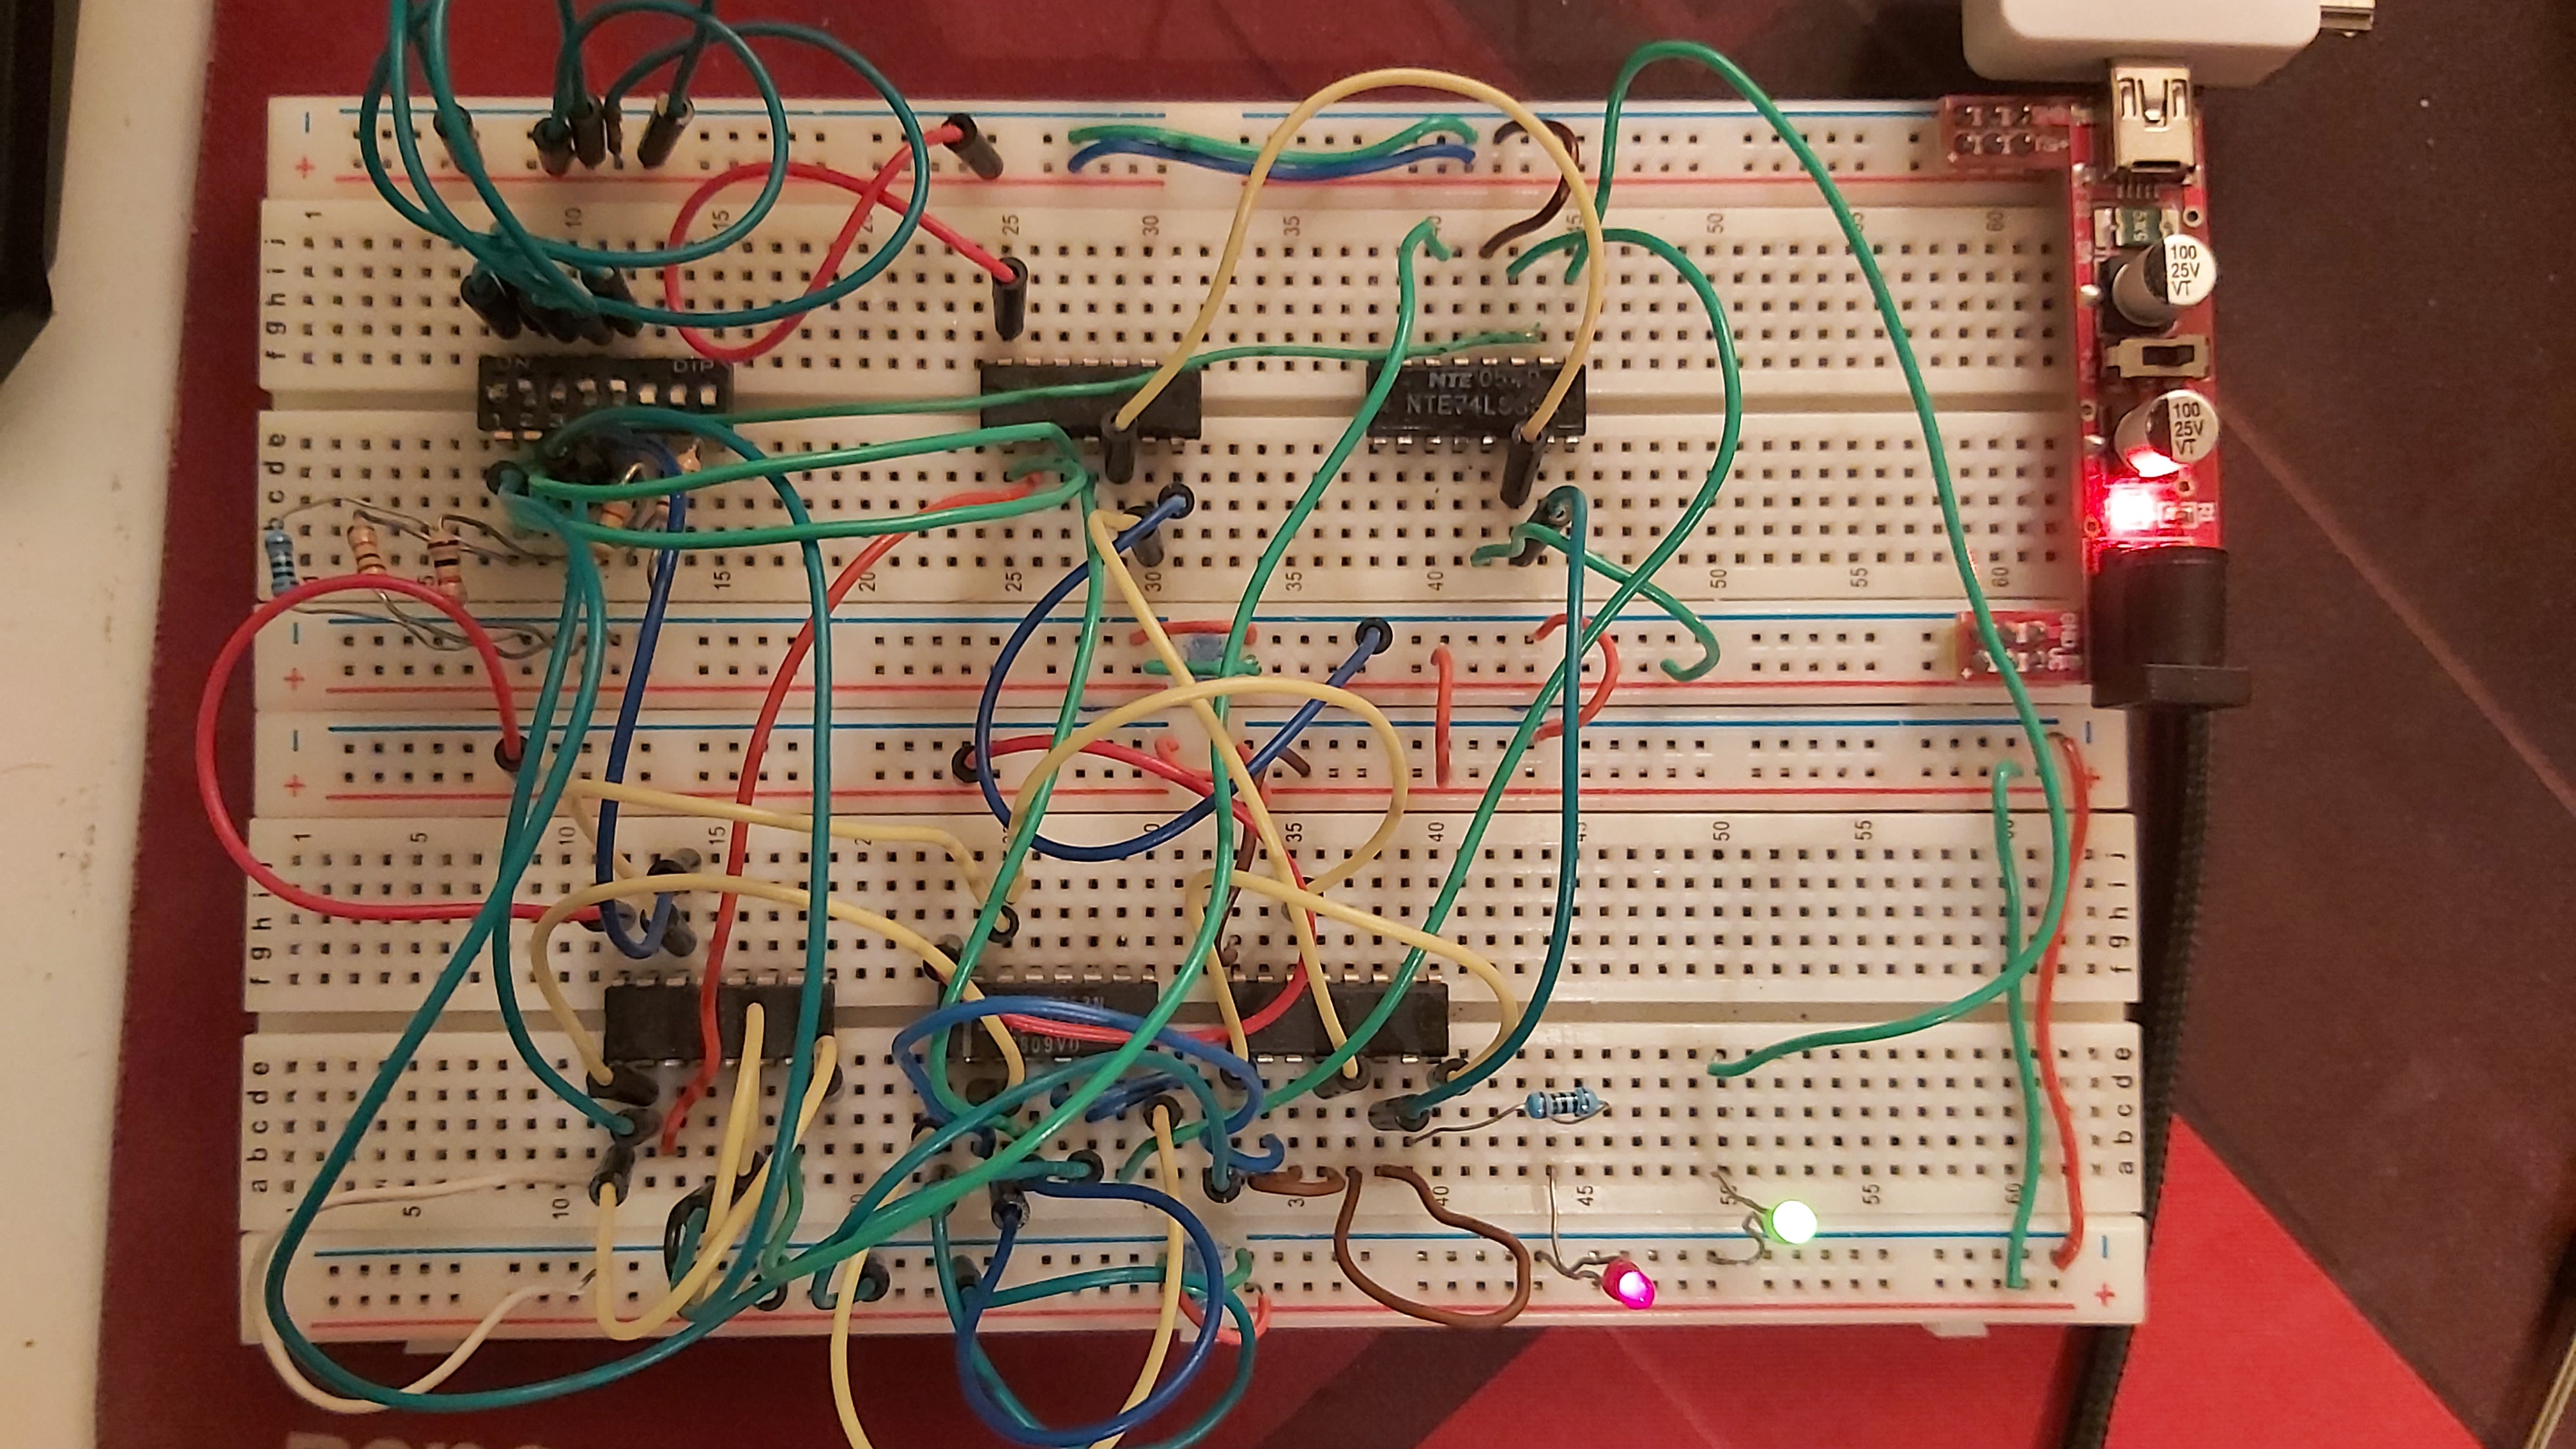
\includegraphics[width=\textwidth]{./figures/01011.jpg}
\begin{center}
	$ABC_i = 010$ and so $C_o Y= 11$.
\end{center}

\vspace{2em}

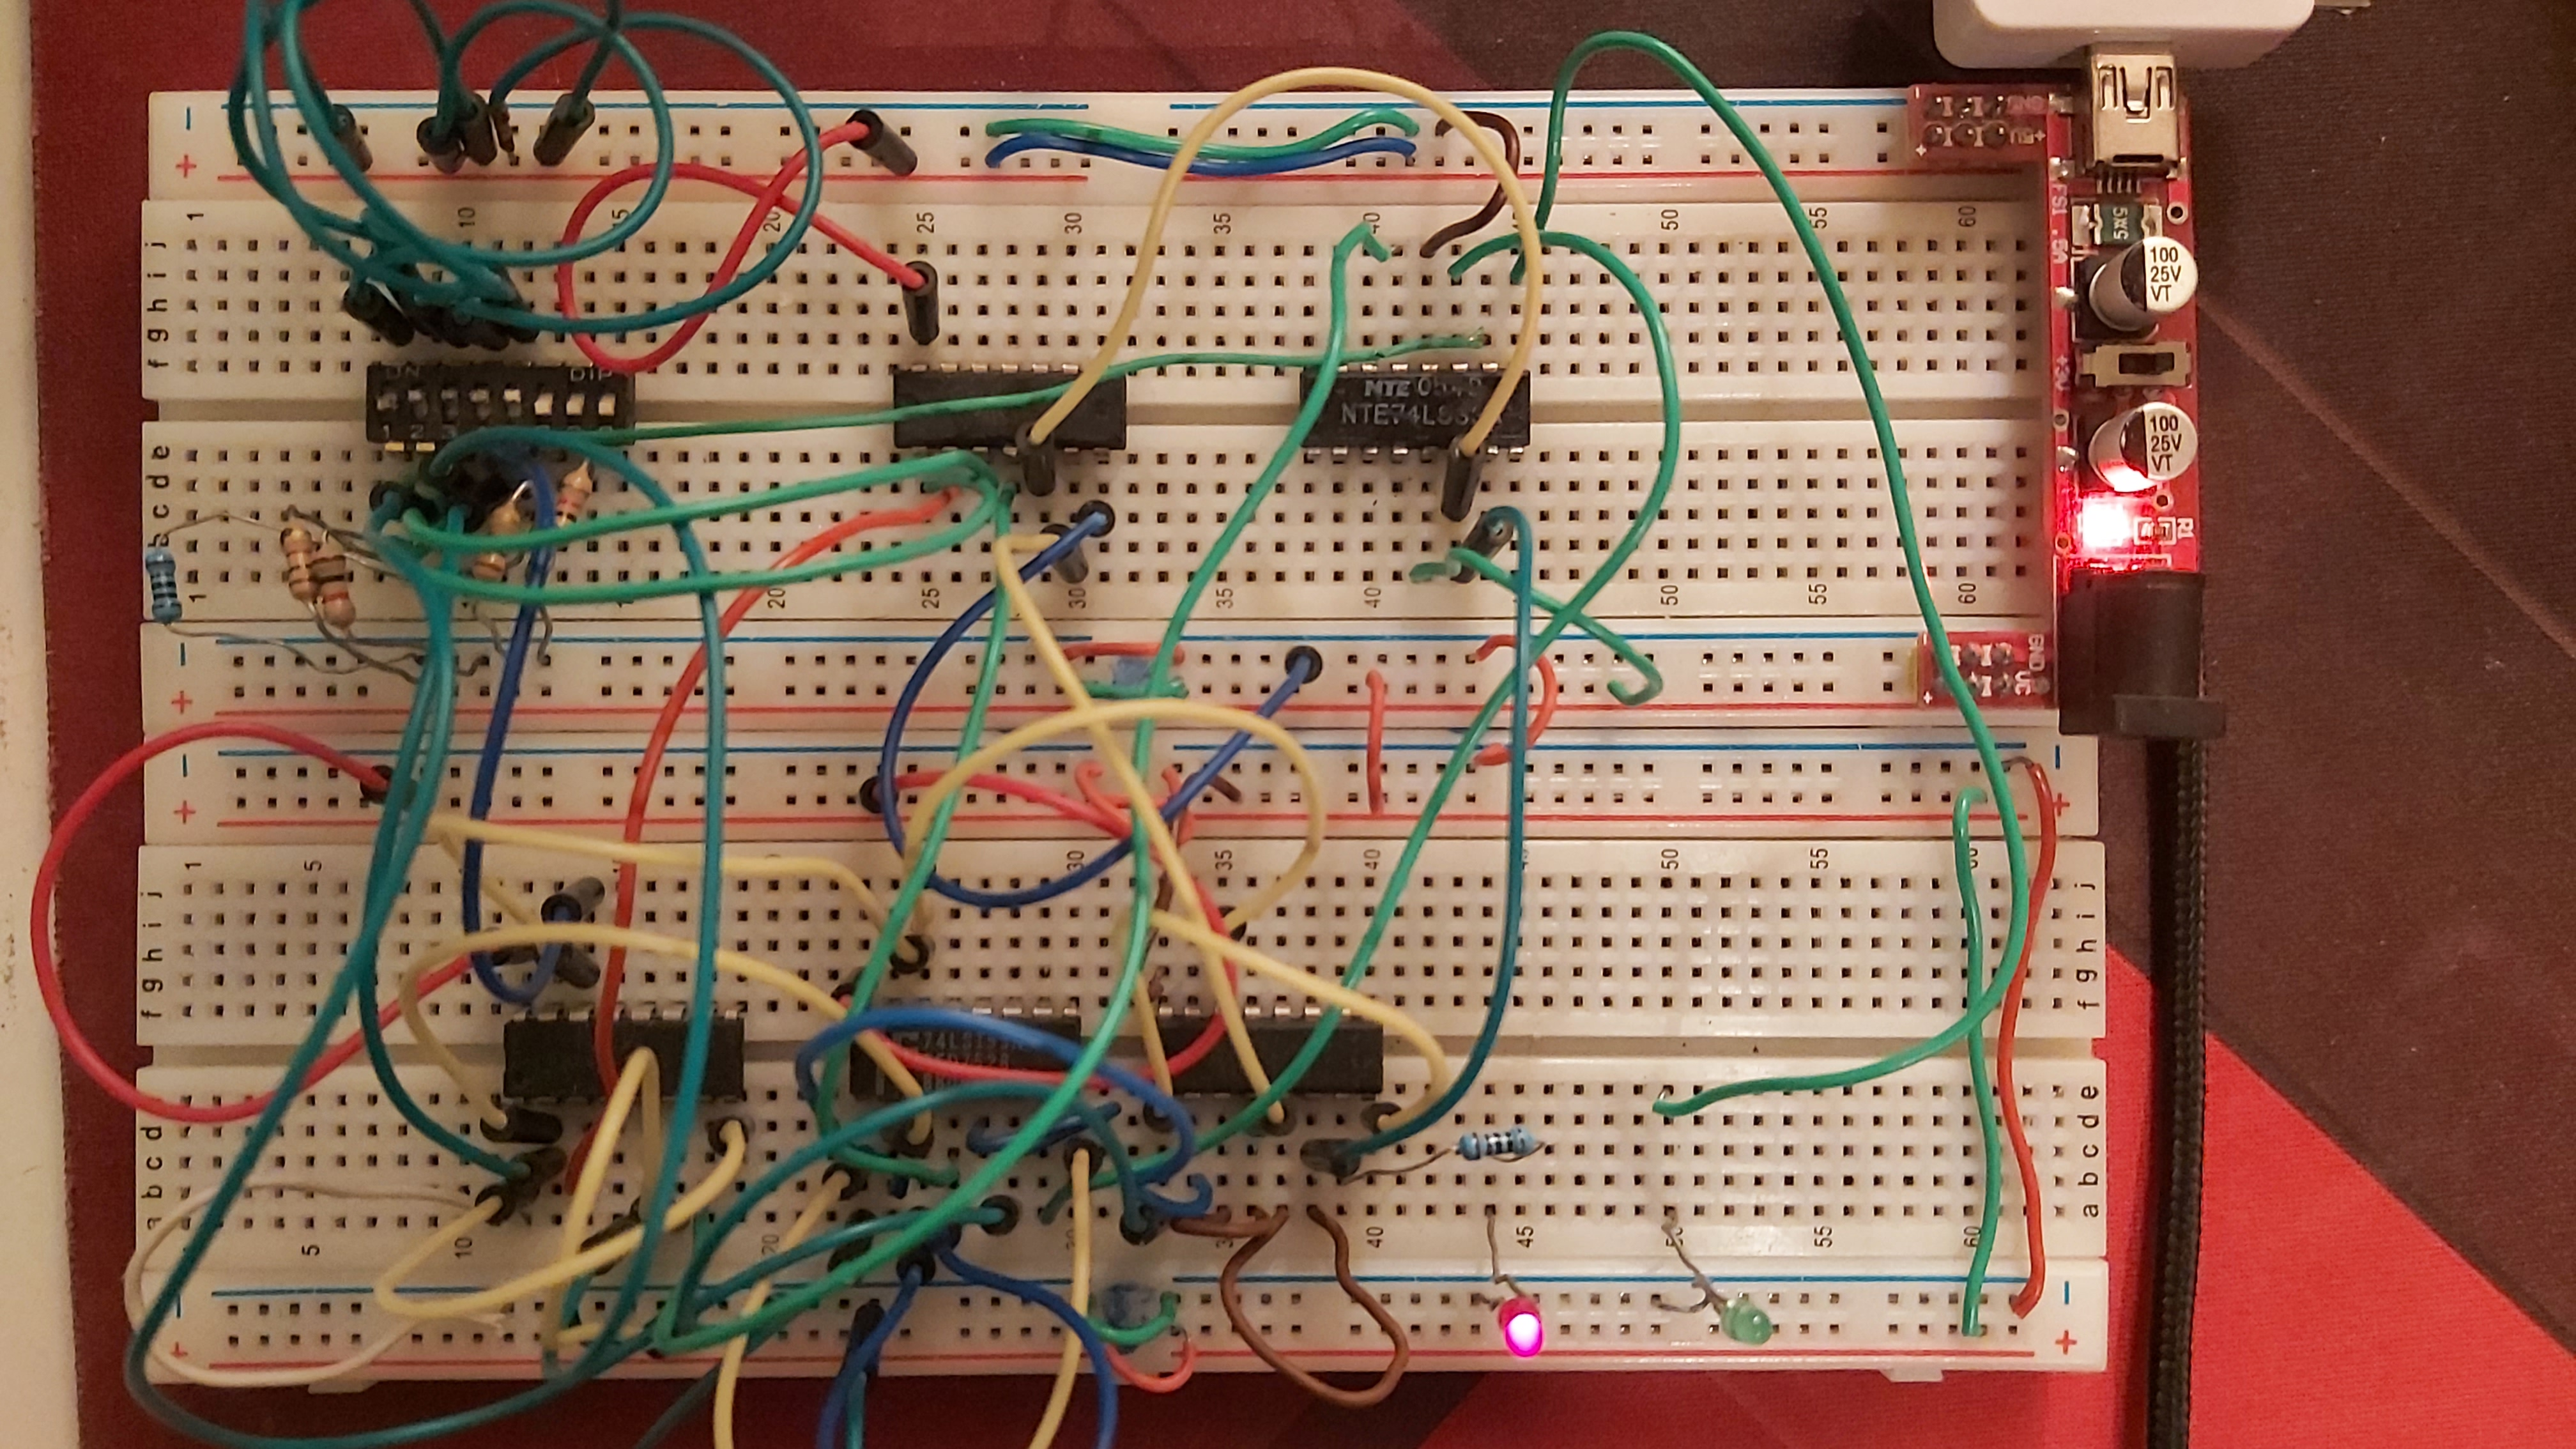
\includegraphics[width=\textwidth]{./figures/01111.jpg}
\begin{center}
	$ABC_i = 011$ and so $C_o Y= 10$.
\end{center}

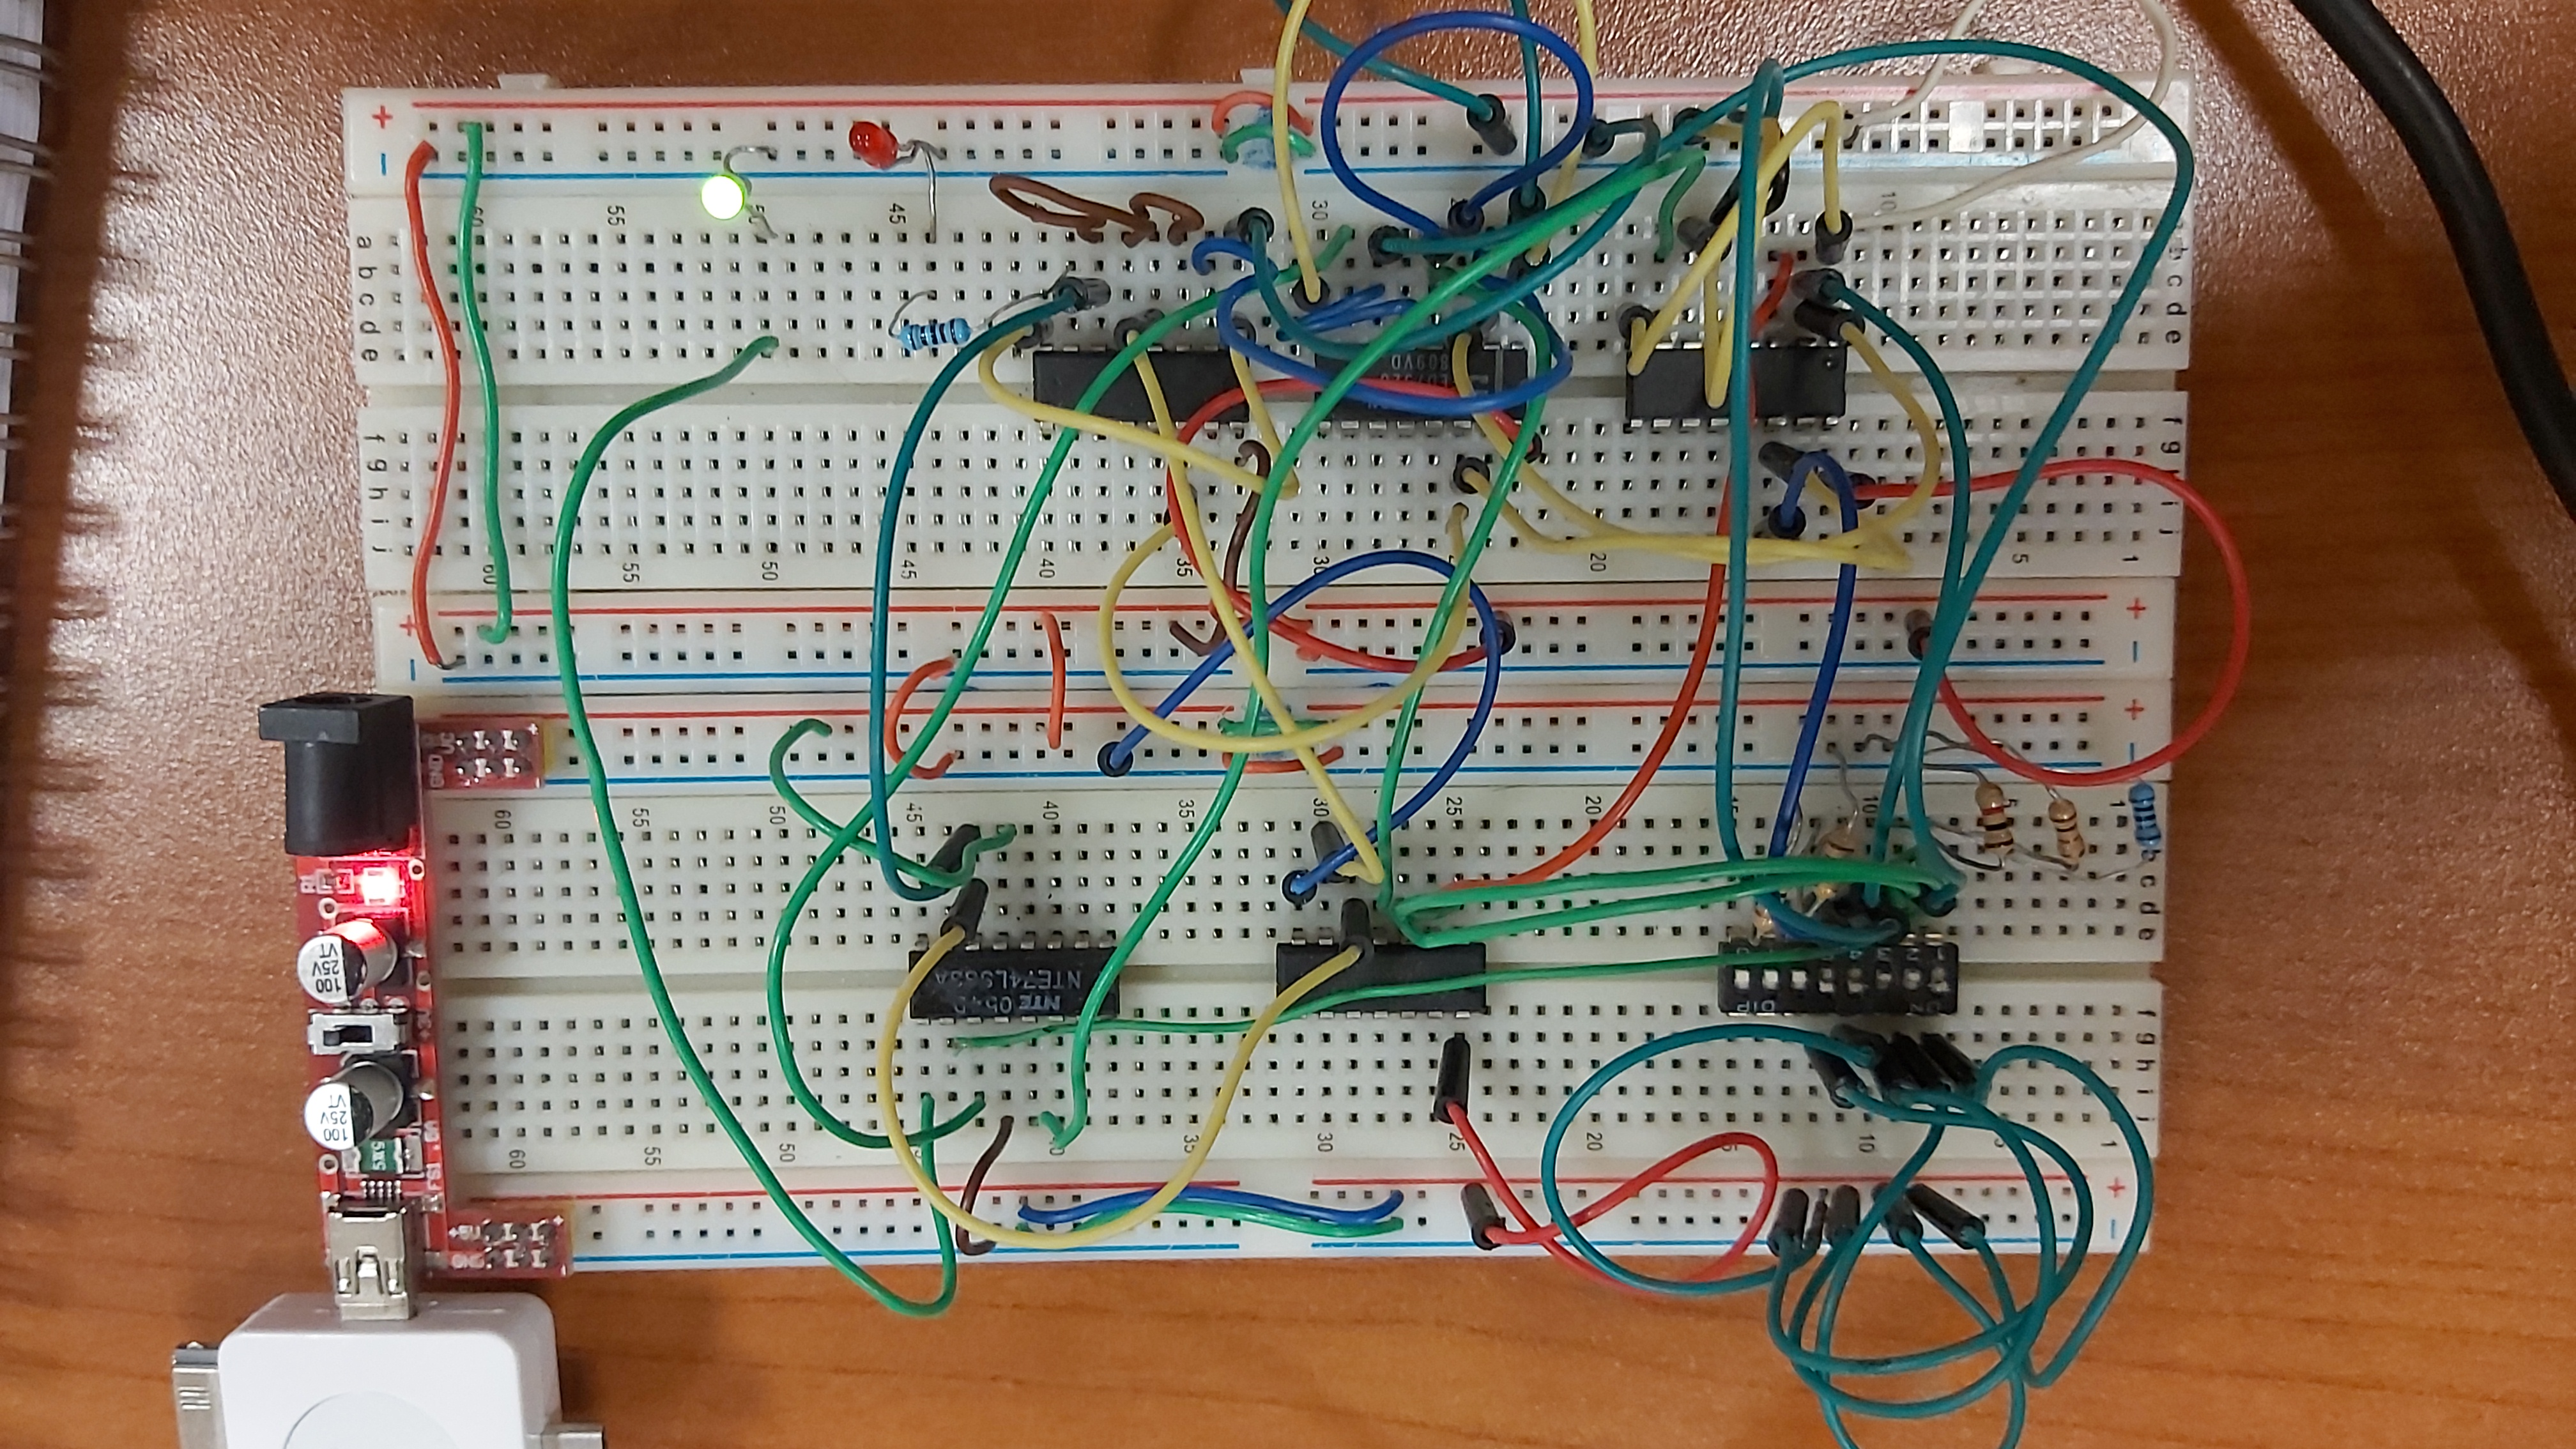
\includegraphics[angle=180, width=\textwidth]{./figures/10011.jpg}
\begin{center}
	$ABC_i = 100$ and so $C_o Y= 01$.
\end{center}

\vspace{2em}

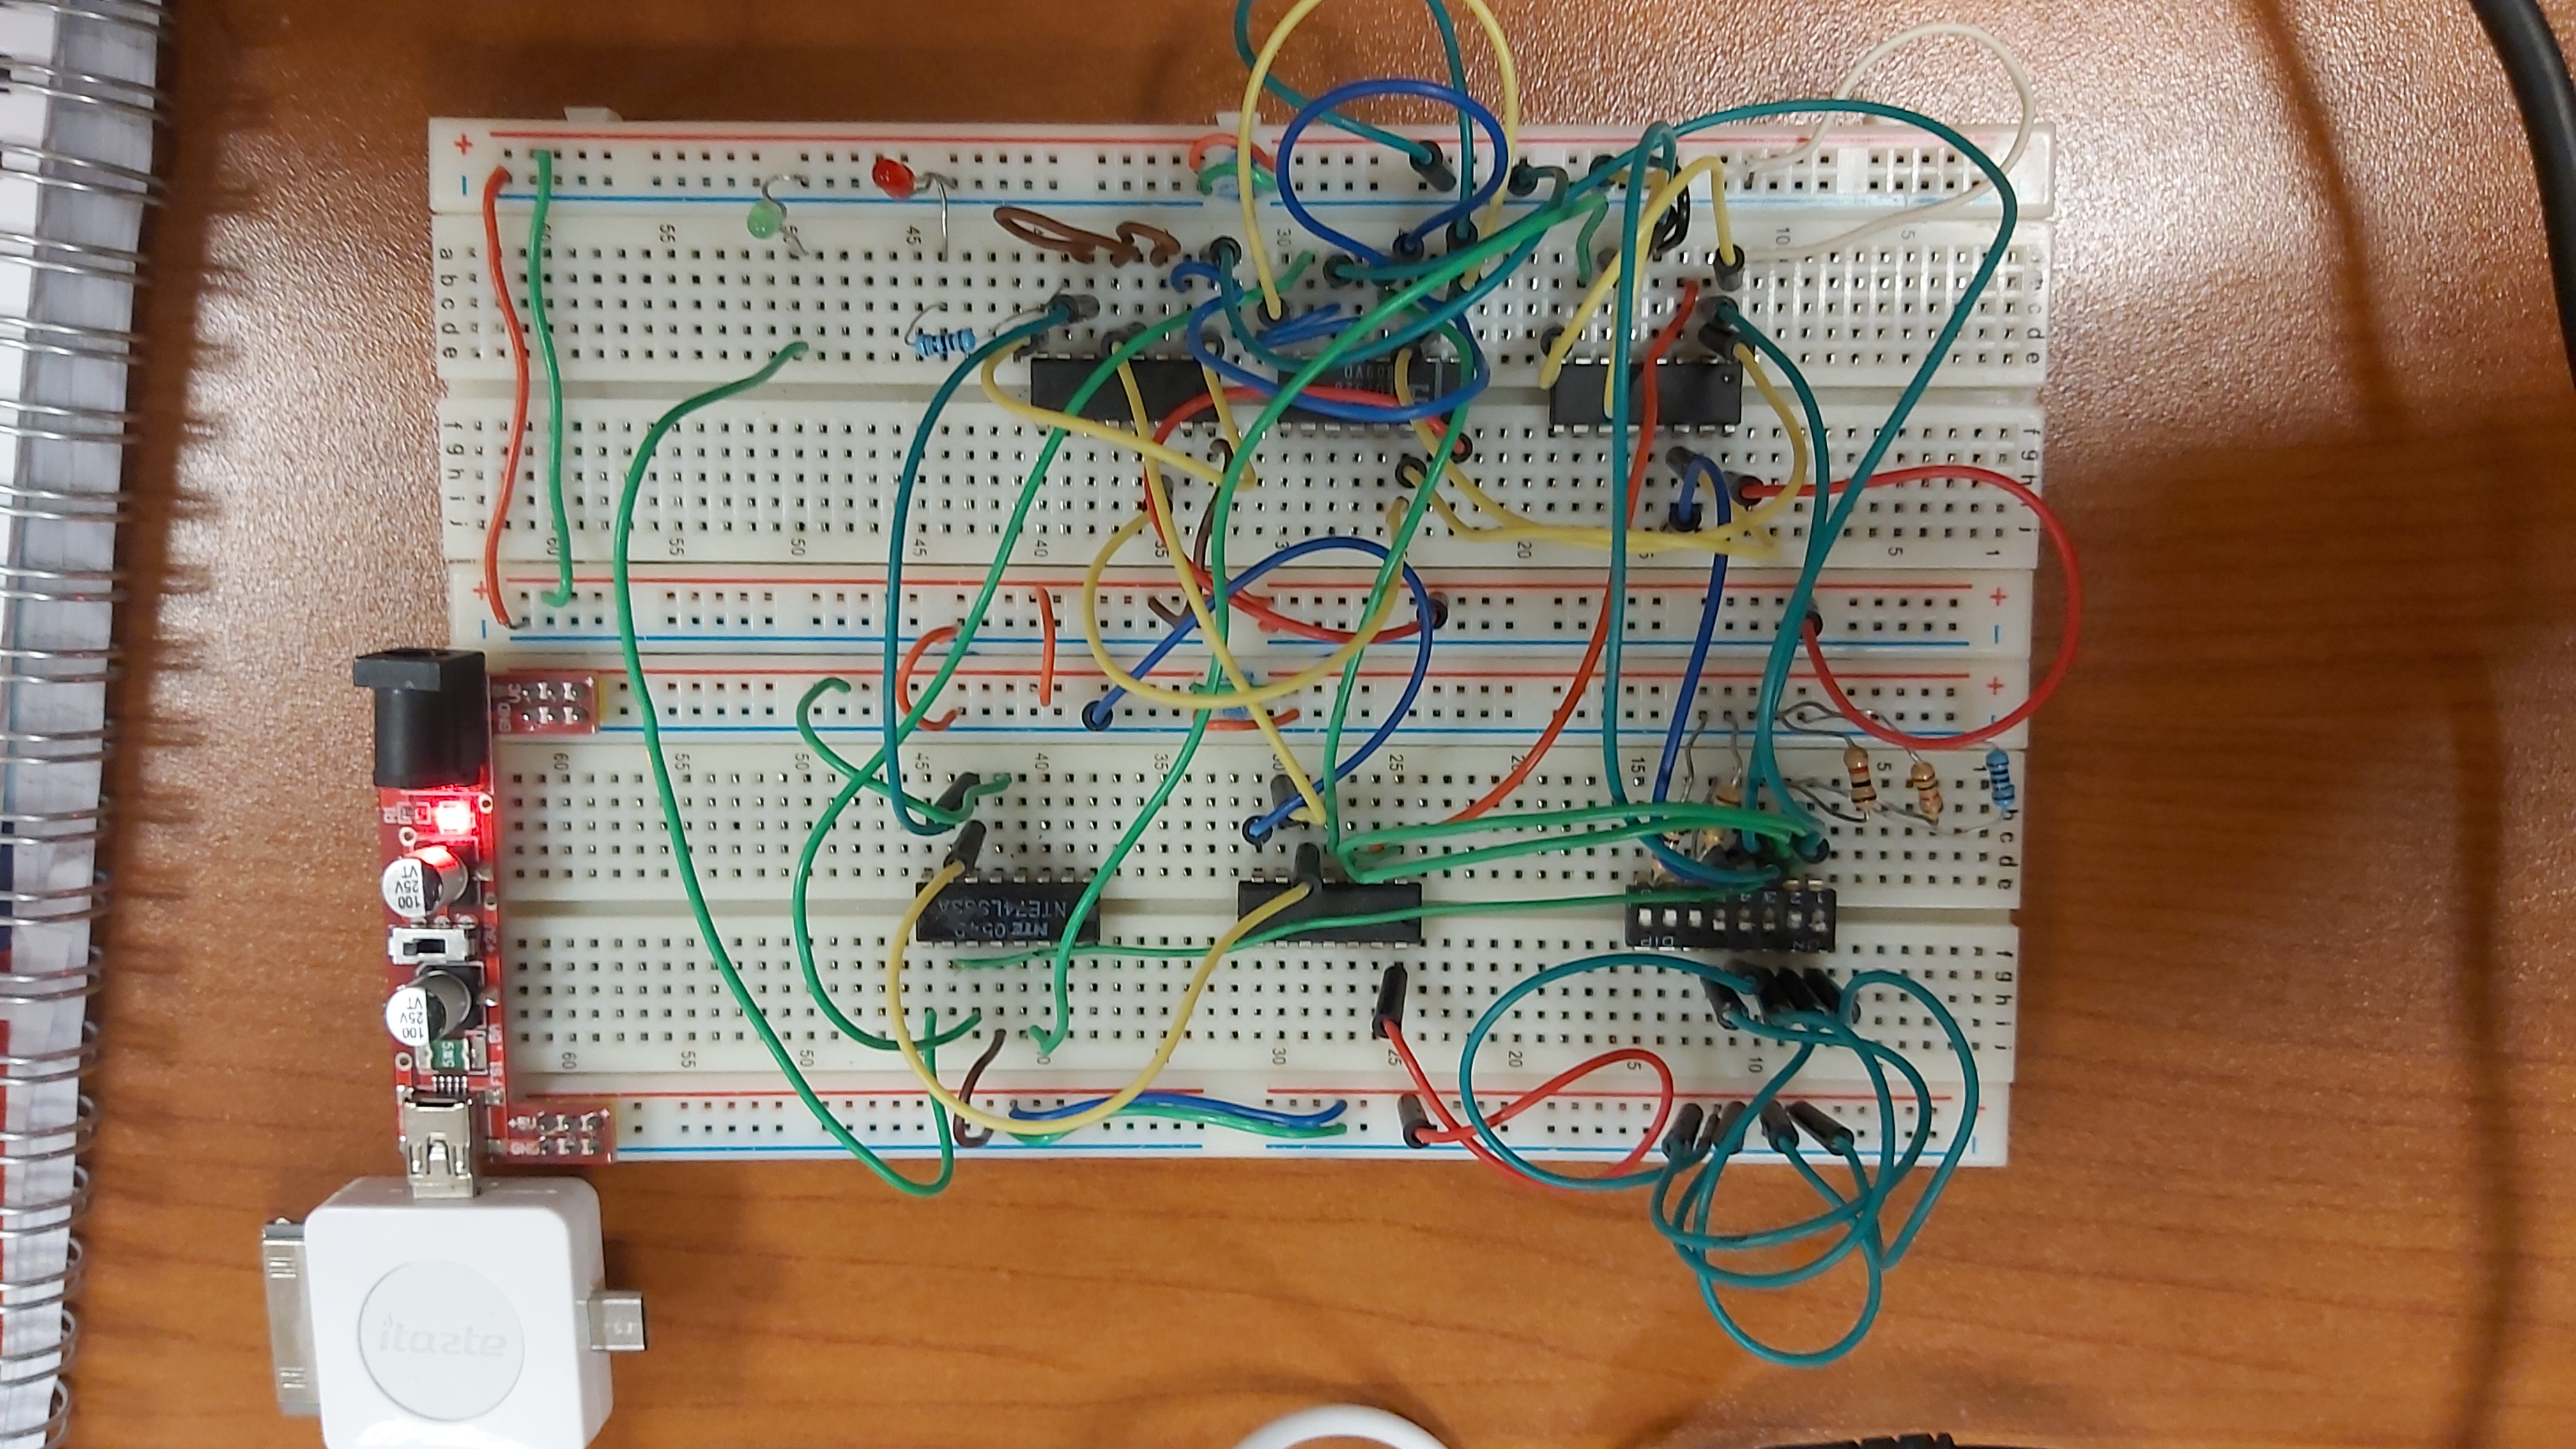
\includegraphics[angle=180, width=\textwidth]{./figures/10111.jpg}
\begin{center}
	$ABC_i = 101$ and so $C_o Y= 00$.
\end{center}

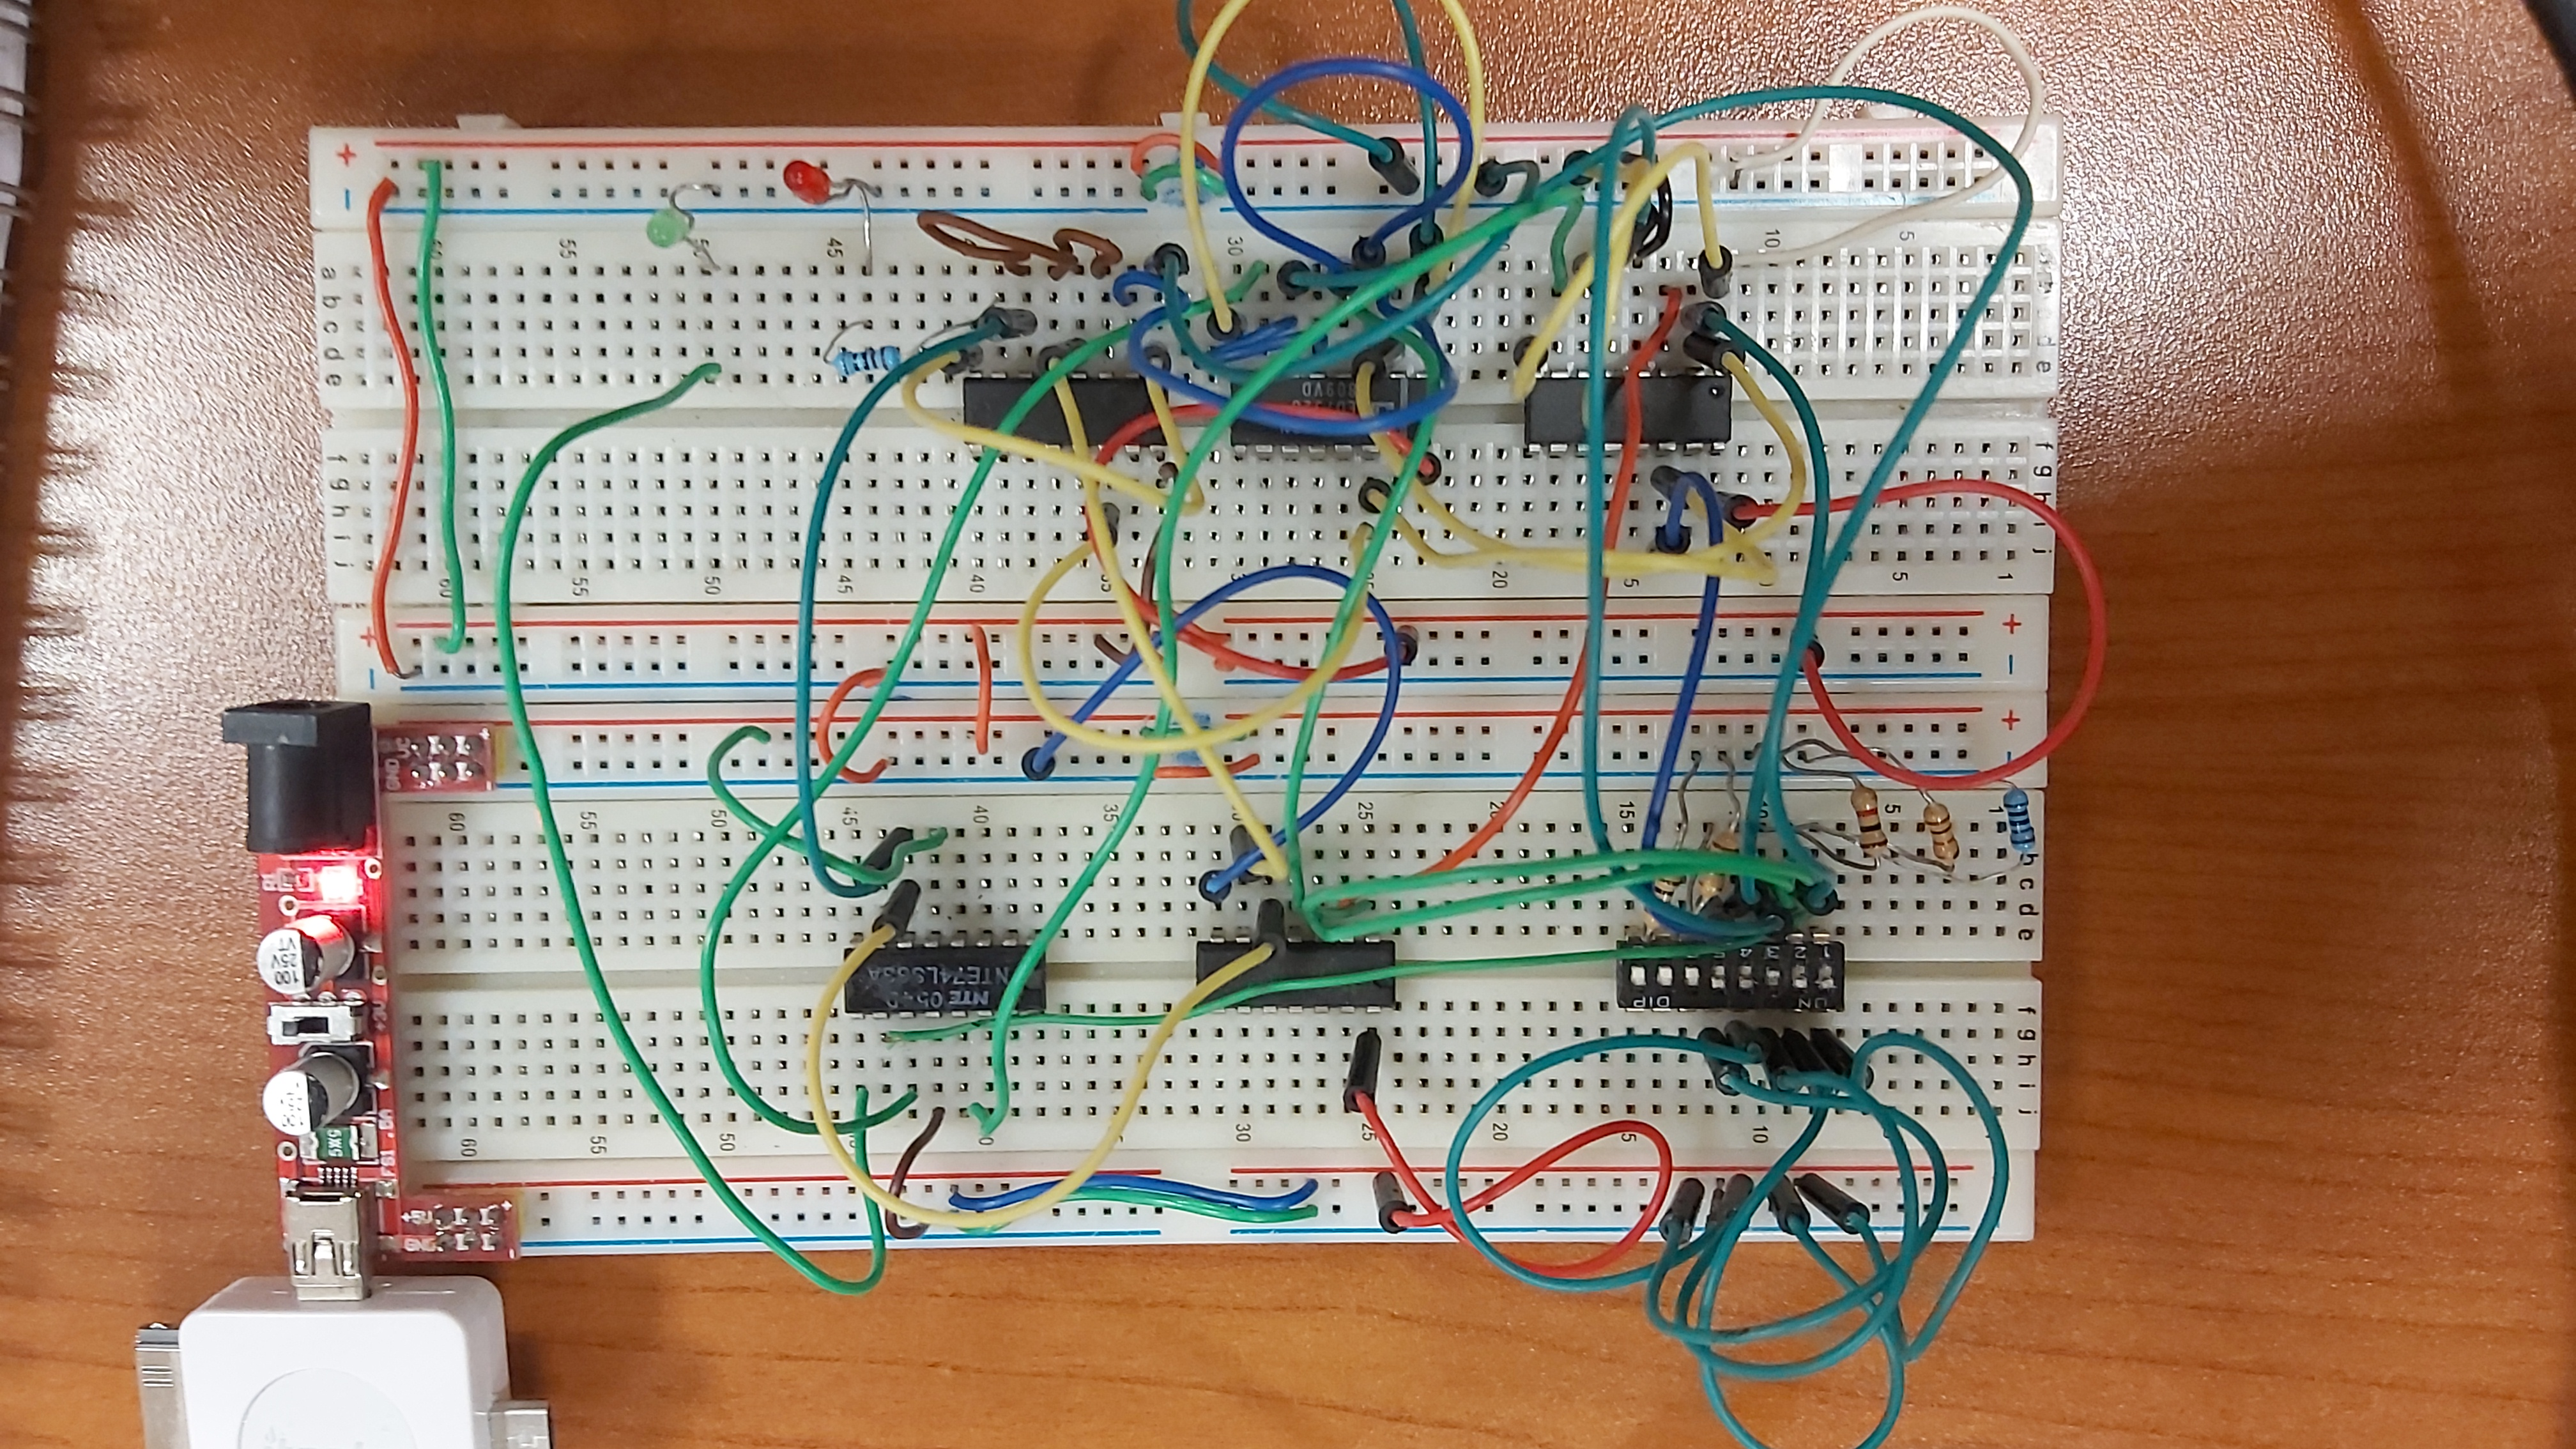
\includegraphics[angle=180, width=\textwidth]{./figures/11011.jpg}
\begin{center}
	$ABC_i = 110$ and so $C_o Y= 00$.
\end{center}

\vspace{2em}

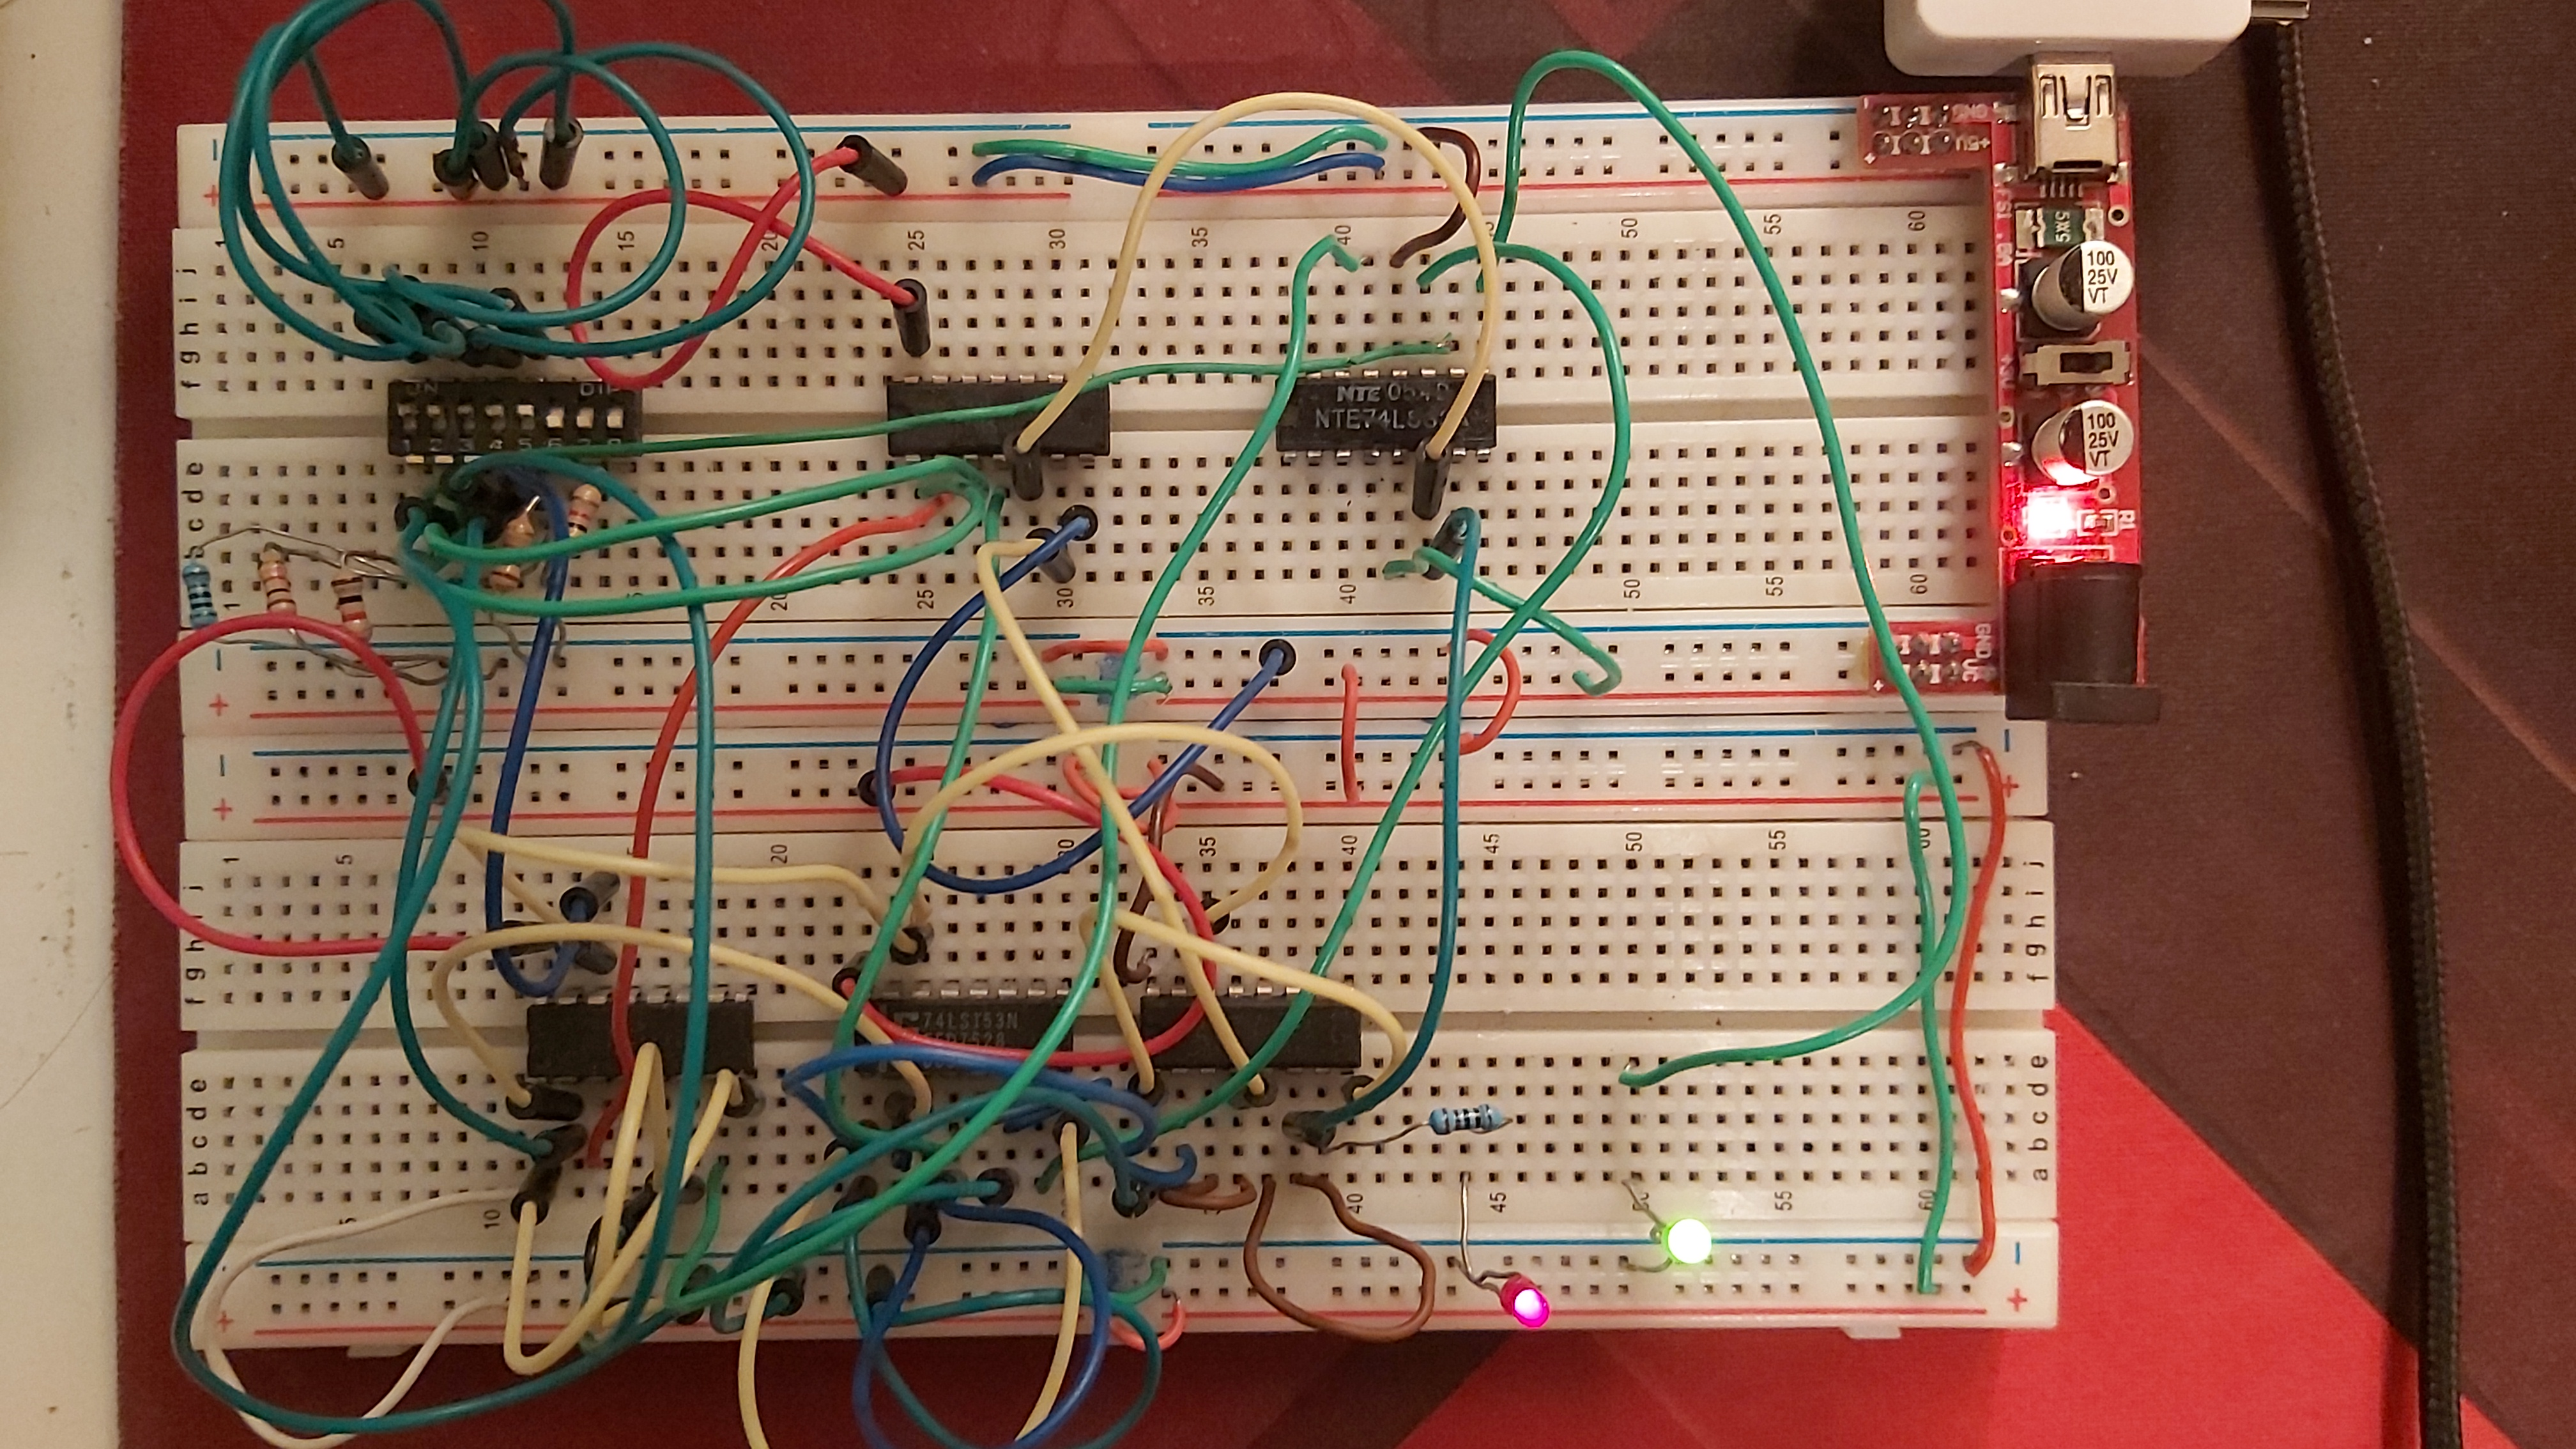
\includegraphics[width=\textwidth]{./figures/11111.jpg}
\begin{center}
	$ABC_i = 111$ and so $C_o Y= 11$.
\end{center}
\end{document}
